%% Before Reading Commits as Learning -- ACM TOCE submission (double-anonymous review version), October 30, 2026
\DocumentMetadata{testphase={phase-III,math,table},pdfstandard=ua-2,lang=en-US}
\documentclass[acmsmall,screen,review,anonymous]{acmart}

\usepackage{booktabs}
\usepackage{multirow}
\usepackage{amsmath}
\usepackage{array}
\usepackage{placeins}
% generated by 38_text_numbers.py from the final result files; do not edit
\makeatletter
\newcommand{\R}[1]{\ifcsname R@#1\endcsname\csname R@#1\endcsname\else\errmessage{Missing result #1}\fi}
\expandafter\def\csname R@agent.N.burst\endcsname{2,875}
\expandafter\def\csname R@agent.N.edit\endcsname{2,875}
\expandafter\def\csname R@agent.N.large\endcsname{2,875}
\expandafter\def\csname R@agent.N.msg\endcsname{2,874}
\expandafter\def\csname R@agent.N.rerun\endcsname{2,875}
\expandafter\def\csname R@agent.N.test\endcsname{2,875}
\expandafter\def\csname R@agent.N.time\endcsname{2,399}
\expandafter\def\csname R@agent.cap100.burst\endcsname{\ensuremath{+0.15}}
\expandafter\def\csname R@agent.cap100.edit\endcsname{\ensuremath{+0.03}}
\expandafter\def\csname R@agent.cap100.large\endcsname{\ensuremath{+0.07}}
\expandafter\def\csname R@agent.cap100.msg\endcsname{\ensuremath{+0.12}}
\expandafter\def\csname R@agent.cap100.rerun\endcsname{\ensuremath{+0.04}}
\expandafter\def\csname R@agent.cap100.test\endcsname{\ensuremath{+0.15}}
\expandafter\def\csname R@agent.cap100.time\endcsname{\ensuremath{+0.07}}
\expandafter\def\csname R@agent.cap100ci.burst\endcsname{\ensuremath{[+0.02, +0.33]}}
\expandafter\def\csname R@agent.cap100ci.edit\endcsname{\ensuremath{[-0.08, +0.17]}}
\expandafter\def\csname R@agent.cap100ci.large\endcsname{\ensuremath{[-0.07, +0.19]}}
\expandafter\def\csname R@agent.cap100ci.msg\endcsname{\ensuremath{[-0.04, +0.25]}}
\expandafter\def\csname R@agent.cap100ci.rerun\endcsname{\ensuremath{[-0.02, +0.10]}}
\expandafter\def\csname R@agent.cap100ci.test\endcsname{\ensuremath{[-0.20, +0.39]}}
\expandafter\def\csname R@agent.cap100ci.time\endcsname{\ensuremath{[-0.09, +0.19]}}
\expandafter\def\csname R@agent.cap100ci95.burst\endcsname{\ensuremath{[-0.01, +0.37]}}
\expandafter\def\csname R@agent.cap100ci95.edit\endcsname{\ensuremath{[-0.11, +0.21]}}
\expandafter\def\csname R@agent.cap100ci95.large\endcsname{\ensuremath{[-0.10, +0.21]}}
\expandafter\def\csname R@agent.cap100ci95.msg\endcsname{\ensuremath{[-0.07, +0.28]}}
\expandafter\def\csname R@agent.cap100ci95.rerun\endcsname{\ensuremath{[-0.02, +0.12]}}
\expandafter\def\csname R@agent.cap100ci95.test\endcsname{\ensuremath{[-0.25, +0.44]}}
\expandafter\def\csname R@agent.cap100ci95.time\endcsname{\ensuremath{[-0.13, +0.22]}}
\expandafter\def\csname R@agent.cap25.burst\endcsname{\ensuremath{+0.20}}
\expandafter\def\csname R@agent.cap25.edit\endcsname{\ensuremath{+0.06}}
\expandafter\def\csname R@agent.cap25.large\endcsname{\ensuremath{+0.06}}
\expandafter\def\csname R@agent.cap25.msg\endcsname{\ensuremath{+0.06}}
\expandafter\def\csname R@agent.cap25.rerun\endcsname{\ensuremath{+0.01}}
\expandafter\def\csname R@agent.cap25.test\endcsname{\ensuremath{+0.02}}
\expandafter\def\csname R@agent.cap25.time\endcsname{\ensuremath{+0.05}}
\expandafter\def\csname R@agent.cap25ci.burst\endcsname{\ensuremath{[+0.05, +0.36]}}
\expandafter\def\csname R@agent.cap25ci.edit\endcsname{\ensuremath{[-0.08, +0.20]}}
\expandafter\def\csname R@agent.cap25ci.large\endcsname{\ensuremath{[-0.07, +0.18]}}
\expandafter\def\csname R@agent.cap25ci.msg\endcsname{\ensuremath{[-0.08, +0.20]}}
\expandafter\def\csname R@agent.cap25ci.rerun\endcsname{\ensuremath{[-0.02, +0.05]}}
\expandafter\def\csname R@agent.cap25ci.test\endcsname{\ensuremath{[-0.19, +0.23]}}
\expandafter\def\csname R@agent.cap25ci.time\endcsname{\ensuremath{[-0.11, +0.18]}}
\expandafter\def\csname R@agent.cap25ci95.burst\endcsname{\ensuremath{[+0.01, +0.38]}}
\expandafter\def\csname R@agent.cap25ci95.edit\endcsname{\ensuremath{[-0.10, +0.22]}}
\expandafter\def\csname R@agent.cap25ci95.large\endcsname{\ensuremath{[-0.09, +0.21]}}
\expandafter\def\csname R@agent.cap25ci95.msg\endcsname{\ensuremath{[-0.11, +0.22]}}
\expandafter\def\csname R@agent.cap25ci95.rerun\endcsname{\ensuremath{[-0.02, +0.06]}}
\expandafter\def\csname R@agent.cap25ci95.test\endcsname{\ensuremath{[-0.21, +0.28]}}
\expandafter\def\csname R@agent.cap25ci95.time\endcsname{\ensuremath{[-0.13, +0.21]}}
\expandafter\def\csname R@agent.cap50.burst\endcsname{\ensuremath{+0.17}}
\expandafter\def\csname R@agent.cap50.edit\endcsname{\ensuremath{+0.05}}
\expandafter\def\csname R@agent.cap50.large\endcsname{\ensuremath{+0.06}}
\expandafter\def\csname R@agent.cap50.msg\endcsname{\ensuremath{+0.08}}
\expandafter\def\csname R@agent.cap50.rerun\endcsname{\ensuremath{+0.02}}
\expandafter\def\csname R@agent.cap50.test\endcsname{\ensuremath{+0.08}}
\expandafter\def\csname R@agent.cap50.time\endcsname{\ensuremath{+0.07}}
\expandafter\def\csname R@agent.cap50ci.burst\endcsname{\ensuremath{[+0.04, +0.35]}}
\expandafter\def\csname R@agent.cap50ci.edit\endcsname{\ensuremath{[-0.08, +0.19]}}
\expandafter\def\csname R@agent.cap50ci.large\endcsname{\ensuremath{[-0.07, +0.18]}}
\expandafter\def\csname R@agent.cap50ci.msg\endcsname{\ensuremath{[-0.06, +0.22]}}
\expandafter\def\csname R@agent.cap50ci.rerun\endcsname{\ensuremath{[-0.02, +0.07]}}
\expandafter\def\csname R@agent.cap50ci.test\endcsname{\ensuremath{[-0.18, +0.31]}}
\expandafter\def\csname R@agent.cap50ci.time\endcsname{\ensuremath{[-0.09, +0.19]}}
\expandafter\def\csname R@agent.cap50ci95.burst\endcsname{\ensuremath{[+0.01, +0.39]}}
\expandafter\def\csname R@agent.cap50ci95.edit\endcsname{\ensuremath{[-0.11, +0.22]}}
\expandafter\def\csname R@agent.cap50ci95.large\endcsname{\ensuremath{[-0.09, +0.21]}}
\expandafter\def\csname R@agent.cap50ci95.msg\endcsname{\ensuremath{[-0.10, +0.24]}}
\expandafter\def\csname R@agent.cap50ci95.rerun\endcsname{\ensuremath{[-0.02, +0.08]}}
\expandafter\def\csname R@agent.cap50ci95.test\endcsname{\ensuremath{[-0.23, +0.36]}}
\expandafter\def\csname R@agent.cap50ci95.time\endcsname{\ensuremath{[-0.12, +0.21]}}
\expandafter\def\csname R@agent.capmax.burst\endcsname{\ensuremath{+0.20}}
\expandafter\def\csname R@agent.capmax.edit\endcsname{\ensuremath{+0.06}}
\expandafter\def\csname R@agent.capmax.large\endcsname{\ensuremath{+0.07}}
\expandafter\def\csname R@agent.capmax.msg\endcsname{\ensuremath{+0.12}}
\expandafter\def\csname R@agent.capmax.rerun\endcsname{\ensuremath{+0.04}}
\expandafter\def\csname R@agent.capmax.size\endcsname{\ensuremath{+0.07}}
\expandafter\def\csname R@agent.capmax.test\endcsname{\ensuremath{+0.15}}
\expandafter\def\csname R@agent.capmax.time\endcsname{\ensuremath{+0.07}}
\expandafter\def\csname R@agent.capmin.burst\endcsname{\ensuremath{+0.15}}
\expandafter\def\csname R@agent.capmin.edit\endcsname{\ensuremath{+0.03}}
\expandafter\def\csname R@agent.capmin.large\endcsname{\ensuremath{+0.06}}
\expandafter\def\csname R@agent.capmin.msg\endcsname{\ensuremath{+0.06}}
\expandafter\def\csname R@agent.capmin.rerun\endcsname{\ensuremath{+0.01}}
\expandafter\def\csname R@agent.capmin.size\endcsname{\ensuremath{+0.03}}
\expandafter\def\csname R@agent.capmin.test\endcsname{\ensuremath{+0.02}}
\expandafter\def\csname R@agent.capmin.time\endcsname{\ensuremath{+0.05}}
\expandafter\def\csname R@agent.cov.burst\endcsname{\ensuremath{-0.35}}
\expandafter\def\csname R@agent.cov.edit\endcsname{\ensuremath{+0.24}}
\expandafter\def\csname R@agent.cov.large\endcsname{\ensuremath{+0.44}}
\expandafter\def\csname R@agent.cov.msg\endcsname{\ensuremath{+0.17}}
\expandafter\def\csname R@agent.cov.rerun\endcsname{\ensuremath{+0.07}}
\expandafter\def\csname R@agent.cov.test\endcsname{\ensuremath{+0.24}}
\expandafter\def\csname R@agent.cov.time\endcsname{\ensuremath{+0.08}}
\expandafter\def\csname R@agent.drop5.burst\endcsname{\ensuremath{+0.25}}
\expandafter\def\csname R@agent.drop5.edit\endcsname{\ensuremath{+0.04}}
\expandafter\def\csname R@agent.drop5.large\endcsname{\ensuremath{+0.02}}
\expandafter\def\csname R@agent.drop5.msg\endcsname{\ensuremath{+0.02}}
\expandafter\def\csname R@agent.drop5.rerun\endcsname{\ensuremath{-0.01}}
\expandafter\def\csname R@agent.drop5.test\endcsname{\ensuremath{-0.02}}
\expandafter\def\csname R@agent.drop5.time\endcsname{\ensuremath{+0.07}}
\expandafter\def\csname R@agent.loo.burst\endcsname{\ensuremath{+0.23}}
\expandafter\def\csname R@agent.loo.edit\endcsname{\ensuremath{+0.02}}
\expandafter\def\csname R@agent.loo.large\endcsname{\ensuremath{+0.02}}
\expandafter\def\csname R@agent.loo.msg\endcsname{\ensuremath{+0.07}}
\expandafter\def\csname R@agent.loo.rerun\endcsname{\ensuremath{+0.09}}
\expandafter\def\csname R@agent.loo.test\endcsname{\ensuremath{-0.05}}
\expandafter\def\csname R@agent.loo.time\endcsname{\ensuremath{+0.10}}
\expandafter\def\csname R@agent.loomax.burst\endcsname{\ensuremath{+0.23}}
\expandafter\def\csname R@agent.loomax.edit\endcsname{\ensuremath{+0.09}}
\expandafter\def\csname R@agent.loomax.large\endcsname{\ensuremath{+0.20}}
\expandafter\def\csname R@agent.loomax.msg\endcsname{\ensuremath{+0.30}}
\expandafter\def\csname R@agent.loomax.rerun\endcsname{\ensuremath{+0.09}}
\expandafter\def\csname R@agent.loomax.test\endcsname{\ensuremath{+0.55}}
\expandafter\def\csname R@agent.loomax.time\endcsname{\ensuremath{+0.10}}
\expandafter\def\csname R@agent.loomin.burst\endcsname{\ensuremath{+0.11}}
\expandafter\def\csname R@agent.loomin.edit\endcsname{\ensuremath{+0.01}}
\expandafter\def\csname R@agent.loomin.large\endcsname{\ensuremath{+0.02}}
\expandafter\def\csname R@agent.loomin.msg\endcsname{\ensuremath{+0.07}}
\expandafter\def\csname R@agent.loomin.rerun\endcsname{\ensuremath{+0.03}}
\expandafter\def\csname R@agent.loomin.test\endcsname{\ensuremath{-0.05}}
\expandafter\def\csname R@agent.loomin.time\endcsname{\ensuremath{-0.03}}
\expandafter\def\csname R@agent.mean0.burst\endcsname{58.5\%}
\expandafter\def\csname R@agent.mean0.large\endcsname{24.0\%}
\expandafter\def\csname R@agent.mean0.test\endcsname{4.8\%}
\expandafter\def\csname R@agent.mean1.burst\endcsname{46.7\%}
\expandafter\def\csname R@agent.mean1.large\endcsname{38.2\%}
\expandafter\def\csname R@agent.mean1.test\endcsname{6.2\%}
\expandafter\def\csname R@agent.n\endcsname{2,875}
\expandafter\def\csname R@agent.nat.burst\endcsname{\ensuremath{+5.5}}
\expandafter\def\csname R@agent.nat.edit\endcsname{+14\%}
\expandafter\def\csname R@agent.nat.large\endcsname{\ensuremath{+1.8}}
\expandafter\def\csname R@agent.nat.test\endcsname{\ensuremath{+1.2}}
\expandafter\def\csname R@agent.natabs.burst\endcsname{5.5}
\expandafter\def\csname R@agent.natabs.edit\endcsname{14\%}
\expandafter\def\csname R@agent.natabs.large\endcsname{1.8}
\expandafter\def\csname R@agent.natabs.test\endcsname{1.2}
\expandafter\def\csname R@agent.natci.burst\endcsname{\ensuremath{[+1.2, +11.2]}}
\expandafter\def\csname R@agent.natci.large\endcsname{\ensuremath{[-2.1, +5.4]}}
\expandafter\def\csname R@agent.natci.test\endcsname{\ensuremath{[-2.6, +4.4]}}
\expandafter\def\csname R@agent.nathi.edit\endcsname{+59\%}
\expandafter\def\csname R@agent.nathiabs.edit\endcsname{59\%}
\expandafter\def\csname R@agent.natlo.edit\endcsname{-19\%}
\expandafter\def\csname R@agent.natloabs.edit\endcsname{19\%}
\expandafter\def\csname R@agent.npost\endcsname{1,267}
\expandafter\def\csname R@agent.npre\endcsname{1,608}
\expandafter\def\csname R@agent.orgs\endcsname{230}
\expandafter\def\csname R@agent.raw.burst\endcsname{\ensuremath{-0.37}}
\expandafter\def\csname R@agent.raw.edit\endcsname{\ensuremath{+0.27}}
\expandafter\def\csname R@agent.raw.large\endcsname{\ensuremath{+0.48}}
\expandafter\def\csname R@agent.raw.msg\endcsname{\ensuremath{+0.19}}
\expandafter\def\csname R@agent.raw.rerun\endcsname{\ensuremath{+0.06}}
\expandafter\def\csname R@agent.raw.test\endcsname{\ensuremath{+0.10}}
\expandafter\def\csname R@agent.raw.time\endcsname{\ensuremath{+0.07}}
\expandafter\def\csname R@agent.ri.burst\endcsname{\ensuremath{+0.11}}
\expandafter\def\csname R@agent.ri.edit\endcsname{\ensuremath{+0.02}}
\expandafter\def\csname R@agent.ri.large\endcsname{\ensuremath{+0.14}}
\expandafter\def\csname R@agent.ri.msg\endcsname{\ensuremath{+0.26}}
\expandafter\def\csname R@agent.ri.rerun\endcsname{\ensuremath{+0.07}}
\expandafter\def\csname R@agent.ri.test\endcsname{\ensuremath{+0.45}}
\expandafter\def\csname R@agent.ri.time\endcsname{\ensuremath{0.00}}
\expandafter\def\csname R@agent.riholm.burst\endcsname{.38}
\expandafter\def\csname R@agent.riholm.edit\endcsname{.99}
\expandafter\def\csname R@agent.riholm.large\endcsname{.11}
\expandafter\def\csname R@agent.riholm.rerun\endcsname{.38}
\expandafter\def\csname R@agent.riholm.test\endcsname{\ensuremath{<}.001}
\expandafter\def\csname R@agent.riholm.time\endcsname{.99}
\expandafter\def\csname R@agent.rip.burst\endcsname{.11}
\expandafter\def\csname R@agent.rip.edit\endcsname{.77}
\expandafter\def\csname R@agent.rip.large\endcsname{.021}
\expandafter\def\csname R@agent.rip.msg\endcsname{\ensuremath{<}.001}
\expandafter\def\csname R@agent.rip.rerun\endcsname{.094}
\expandafter\def\csname R@agent.rip.test\endcsname{\ensuremath{<}.001}
\expandafter\def\csname R@agent.rip.time\endcsname{.99}
\expandafter\def\csname R@agent.w.burst\endcsname{\ensuremath{+0.16}}
\expandafter\def\csname R@agent.w.edit\endcsname{\ensuremath{+0.17}}
\expandafter\def\csname R@agent.w.large\endcsname{\ensuremath{+0.35}}
\expandafter\def\csname R@agent.w.msg\endcsname{\ensuremath{+0.45}}
\expandafter\def\csname R@agent.w.rerun\endcsname{\ensuremath{+0.04}}
\expandafter\def\csname R@agent.w.test\endcsname{\ensuremath{+0.87}}
\expandafter\def\csname R@agent.w.time\endcsname{\ensuremath{-0.28}}
\expandafter\def\csname R@agent.wp.burst\endcsname{.21}
\expandafter\def\csname R@agent.wp.edit\endcsname{.14}
\expandafter\def\csname R@agent.wp.large\endcsname{.44}
\expandafter\def\csname R@agent.wp.msg\endcsname{.40}
\expandafter\def\csname R@agent.wp.rerun\endcsname{.43}
\expandafter\def\csname R@agent.wp.test\endcsname{.64}
\expandafter\def\csname R@agent.wp.time\endcsname{.41}
\expandafter\def\csname R@agent.wpmax\endcsname{.64}
\expandafter\def\csname R@agent.wpmin\endcsname{.14}
\expandafter\def\csname R@agent.wrange.burst\endcsname{\ensuremath{[-1.0, +1.4]}}
\expandafter\def\csname R@agent.wrange.edit\endcsname{\ensuremath{[-3.4, +3.8]}}
\expandafter\def\csname R@agent.wrange.large\endcsname{\ensuremath{[-1.3, +2.0]}}
\expandafter\def\csname R@agent.wrange.msg\endcsname{\ensuremath{[-1.5, +2.4]}}
\expandafter\def\csname R@agent.wrange.rerun\endcsname{\ensuremath{[-0.2, +0.3]}}
\expandafter\def\csname R@agent.wrange.test\endcsname{\ensuremath{[-8.4, +10.1]}}
\expandafter\def\csname R@agent.wrange.time\endcsname{\ensuremath{[-1.7, +1.2]}}
\expandafter\def\csname R@copies.maxmove.bound\endcsname{0.08}
\expandafter\def\csname R@copies.maxmove.cap\endcsname{0.07}
\expandafter\def\csname R@copies.maxmove.ri\endcsname{0.08}
\expandafter\def\csname R@era.N.burst\endcsname{4,941}
\expandafter\def\csname R@era.N.edit\endcsname{4,940}
\expandafter\def\csname R@era.N.large\endcsname{4,940}
\expandafter\def\csname R@era.N.msg\endcsname{4,915}
\expandafter\def\csname R@era.N.rerun\endcsname{4,941}
\expandafter\def\csname R@era.N.test\endcsname{4,941}
\expandafter\def\csname R@era.N.time\endcsname{4,106}
\expandafter\def\csname R@era.cap100.burst\endcsname{\ensuremath{+0.12}}
\expandafter\def\csname R@era.cap100.edit\endcsname{\ensuremath{-0.11}}
\expandafter\def\csname R@era.cap100.large\endcsname{\ensuremath{-0.05}}
\expandafter\def\csname R@era.cap100.msg\endcsname{\ensuremath{-0.18}}
\expandafter\def\csname R@era.cap100.rerun\endcsname{\ensuremath{+0.02}}
\expandafter\def\csname R@era.cap100.test\endcsname{\ensuremath{-0.08}}
\expandafter\def\csname R@era.cap100.time\endcsname{\ensuremath{-0.02}}
\expandafter\def\csname R@era.cap100ci.burst\endcsname{\ensuremath{[-0.03, +0.26]}}
\expandafter\def\csname R@era.cap100ci.edit\endcsname{\ensuremath{[-0.28, +0.08]}}
\expandafter\def\csname R@era.cap100ci.large\endcsname{\ensuremath{[-0.19, +0.09]}}
\expandafter\def\csname R@era.cap100ci.msg\endcsname{\ensuremath{[-0.27, -0.06]}}
\expandafter\def\csname R@era.cap100ci.rerun\endcsname{\ensuremath{[-0.001, +0.06]}}
\expandafter\def\csname R@era.cap100ci.test\endcsname{\ensuremath{[-0.23, +0.03]}}
\expandafter\def\csname R@era.cap100ci.time\endcsname{\ensuremath{[-0.10, +0.07]}}
\expandafter\def\csname R@era.cap100ci95.burst\endcsname{\ensuremath{[-0.05, +0.29]}}
\expandafter\def\csname R@era.cap100ci95.edit\endcsname{\ensuremath{[-0.31, +0.12]}}
\expandafter\def\csname R@era.cap100ci95.large\endcsname{\ensuremath{[-0.21, +0.12]}}
\expandafter\def\csname R@era.cap100ci95.msg\endcsname{\ensuremath{[-0.28, -0.05]}}
\expandafter\def\csname R@era.cap100ci95.rerun\endcsname{\ensuremath{[-0.004, +0.06]}}
\expandafter\def\csname R@era.cap100ci95.test\endcsname{\ensuremath{[-0.26, +0.05]}}
\expandafter\def\csname R@era.cap100ci95.time\endcsname{\ensuremath{[-0.12, +0.09]}}
\expandafter\def\csname R@era.cap25.burst\endcsname{\ensuremath{+0.05}}
\expandafter\def\csname R@era.cap25.edit\endcsname{\ensuremath{+0.02}}
\expandafter\def\csname R@era.cap25.large\endcsname{\ensuremath{+0.04}}
\expandafter\def\csname R@era.cap25.msg\endcsname{\ensuremath{-0.17}}
\expandafter\def\csname R@era.cap25.rerun\endcsname{\ensuremath{+0.01}}
\expandafter\def\csname R@era.cap25.test\endcsname{\ensuremath{-0.10}}
\expandafter\def\csname R@era.cap25.time\endcsname{\ensuremath{0.00}}
\expandafter\def\csname R@era.cap25ci.burst\endcsname{\ensuremath{[-0.09, +0.17]}}
\expandafter\def\csname R@era.cap25ci.edit\endcsname{\ensuremath{[-0.09, +0.14]}}
\expandafter\def\csname R@era.cap25ci.large\endcsname{\ensuremath{[-0.08, +0.14]}}
\expandafter\def\csname R@era.cap25ci.msg\endcsname{\ensuremath{[-0.26, -0.07]}}
\expandafter\def\csname R@era.cap25ci.rerun\endcsname{\ensuremath{[-0.003, +0.04]}}
\expandafter\def\csname R@era.cap25ci.test\endcsname{\ensuremath{[-0.24, +0.04]}}
\expandafter\def\csname R@era.cap25ci.time\endcsname{\ensuremath{[-0.09, +0.10]}}
\expandafter\def\csname R@era.cap25ci95.burst\endcsname{\ensuremath{[-0.11, +0.19]}}
\expandafter\def\csname R@era.cap25ci95.edit\endcsname{\ensuremath{[-0.11, +0.16]}}
\expandafter\def\csname R@era.cap25ci95.large\endcsname{\ensuremath{[-0.10, +0.16]}}
\expandafter\def\csname R@era.cap25ci95.msg\endcsname{\ensuremath{[-0.28, -0.05]}}
\expandafter\def\csname R@era.cap25ci95.rerun\endcsname{\ensuremath{[-0.005, +0.05]}}
\expandafter\def\csname R@era.cap25ci95.test\endcsname{\ensuremath{[-0.26, +0.06]}}
\expandafter\def\csname R@era.cap25ci95.time\endcsname{\ensuremath{[-0.11, +0.12]}}
\expandafter\def\csname R@era.cap50.burst\endcsname{\ensuremath{+0.08}}
\expandafter\def\csname R@era.cap50.edit\endcsname{\ensuremath{-0.03}}
\expandafter\def\csname R@era.cap50.large\endcsname{\ensuremath{0.00}}
\expandafter\def\csname R@era.cap50.msg\endcsname{\ensuremath{-0.17}}
\expandafter\def\csname R@era.cap50.rerun\endcsname{\ensuremath{+0.02}}
\expandafter\def\csname R@era.cap50.test\endcsname{\ensuremath{-0.09}}
\expandafter\def\csname R@era.cap50.time\endcsname{\ensuremath{-0.02}}
\expandafter\def\csname R@era.cap50ci.burst\endcsname{\ensuremath{[-0.07, +0.21]}}
\expandafter\def\csname R@era.cap50ci.edit\endcsname{\ensuremath{[-0.17, +0.11]}}
\expandafter\def\csname R@era.cap50ci.large\endcsname{\ensuremath{[-0.12, +0.12]}}
\expandafter\def\csname R@era.cap50ci.msg\endcsname{\ensuremath{[-0.27, -0.07]}}
\expandafter\def\csname R@era.cap50ci.rerun\endcsname{\ensuremath{[-0.003, +0.05]}}
\expandafter\def\csname R@era.cap50ci.test\endcsname{\ensuremath{[-0.21, +0.02]}}
\expandafter\def\csname R@era.cap50ci.time\endcsname{\ensuremath{[-0.10, +0.08]}}
\expandafter\def\csname R@era.cap50ci95.burst\endcsname{\ensuremath{[-0.10, +0.23]}}
\expandafter\def\csname R@era.cap50ci95.edit\endcsname{\ensuremath{[-0.18, +0.14]}}
\expandafter\def\csname R@era.cap50ci95.large\endcsname{\ensuremath{[-0.14, +0.14]}}
\expandafter\def\csname R@era.cap50ci95.msg\endcsname{\ensuremath{[-0.28, -0.05]}}
\expandafter\def\csname R@era.cap50ci95.rerun\endcsname{\ensuremath{[-0.01, +0.05]}}
\expandafter\def\csname R@era.cap50ci95.test\endcsname{\ensuremath{[-0.24, +0.04]}}
\expandafter\def\csname R@era.cap50ci95.time\endcsname{\ensuremath{[-0.12, +0.09]}}
\expandafter\def\csname R@era.capmax.burst\endcsname{\ensuremath{+0.12}}
\expandafter\def\csname R@era.capmax.edit\endcsname{\ensuremath{+0.02}}
\expandafter\def\csname R@era.capmax.large\endcsname{\ensuremath{+0.04}}
\expandafter\def\csname R@era.capmax.msg\endcsname{\ensuremath{-0.17}}
\expandafter\def\csname R@era.capmax.rerun\endcsname{\ensuremath{+0.02}}
\expandafter\def\csname R@era.capmax.size\endcsname{\ensuremath{+0.04}}
\expandafter\def\csname R@era.capmax.test\endcsname{\ensuremath{-0.08}}
\expandafter\def\csname R@era.capmax.time\endcsname{\ensuremath{0.00}}
\expandafter\def\csname R@era.capmin.burst\endcsname{\ensuremath{+0.05}}
\expandafter\def\csname R@era.capmin.edit\endcsname{\ensuremath{-0.11}}
\expandafter\def\csname R@era.capmin.large\endcsname{\ensuremath{-0.05}}
\expandafter\def\csname R@era.capmin.msg\endcsname{\ensuremath{-0.18}}
\expandafter\def\csname R@era.capmin.rerun\endcsname{\ensuremath{+0.01}}
\expandafter\def\csname R@era.capmin.size\endcsname{\ensuremath{-0.11}}
\expandafter\def\csname R@era.capmin.test\endcsname{\ensuremath{-0.10}}
\expandafter\def\csname R@era.capmin.time\endcsname{\ensuremath{-0.02}}
\expandafter\def\csname R@era.cov.burst\endcsname{\ensuremath{+0.04}}
\expandafter\def\csname R@era.cov.edit\endcsname{\ensuremath{+0.15}}
\expandafter\def\csname R@era.cov.large\endcsname{\ensuremath{+0.23}}
\expandafter\def\csname R@era.cov.msg\endcsname{\ensuremath{-0.36}}
\expandafter\def\csname R@era.cov.rerun\endcsname{\ensuremath{+0.05}}
\expandafter\def\csname R@era.cov.test\endcsname{\ensuremath{-0.16}}
\expandafter\def\csname R@era.cov.time\endcsname{\ensuremath{-0.07}}
\expandafter\def\csname R@era.drop5.burst\endcsname{\ensuremath{+0.07}}
\expandafter\def\csname R@era.drop5.edit\endcsname{\ensuremath{-0.03}}
\expandafter\def\csname R@era.drop5.large\endcsname{\ensuremath{-0.01}}
\expandafter\def\csname R@era.drop5.msg\endcsname{\ensuremath{-0.10}}
\expandafter\def\csname R@era.drop5.rerun\endcsname{\ensuremath{0.00}}
\expandafter\def\csname R@era.drop5.test\endcsname{\ensuremath{-0.07}}
\expandafter\def\csname R@era.drop5.time\endcsname{\ensuremath{+0.01}}
\expandafter\def\csname R@era.loo.burst\endcsname{\ensuremath{+0.03}}
\expandafter\def\csname R@era.loo.edit\endcsname{\ensuremath{-0.03}}
\expandafter\def\csname R@era.loo.large\endcsname{\ensuremath{+0.03}}
\expandafter\def\csname R@era.loo.msg\endcsname{\ensuremath{-0.20}}
\expandafter\def\csname R@era.loo.rerun\endcsname{\ensuremath{+0.05}}
\expandafter\def\csname R@era.loo.test\endcsname{\ensuremath{+0.01}}
\expandafter\def\csname R@era.loo.time\endcsname{\ensuremath{-0.03}}
\expandafter\def\csname R@era.loomax.burst\endcsname{\ensuremath{+0.39}}
\expandafter\def\csname R@era.loomax.edit\endcsname{\ensuremath{-0.03}}
\expandafter\def\csname R@era.loomax.large\endcsname{\ensuremath{+0.03}}
\expandafter\def\csname R@era.loomax.msg\endcsname{\ensuremath{-0.13}}
\expandafter\def\csname R@era.loomax.rerun\endcsname{\ensuremath{+0.05}}
\expandafter\def\csname R@era.loomax.test\endcsname{\ensuremath{+0.01}}
\expandafter\def\csname R@era.loomax.time\endcsname{\ensuremath{-0.03}}
\expandafter\def\csname R@era.loomin.burst\endcsname{\ensuremath{+0.03}}
\expandafter\def\csname R@era.loomin.edit\endcsname{\ensuremath{-0.39}}
\expandafter\def\csname R@era.loomin.large\endcsname{\ensuremath{-0.27}}
\expandafter\def\csname R@era.loomin.msg\endcsname{\ensuremath{-0.23}}
\expandafter\def\csname R@era.loomin.rerun\endcsname{\ensuremath{+0.02}}
\expandafter\def\csname R@era.loomin.test\endcsname{\ensuremath{-0.27}}
\expandafter\def\csname R@era.loomin.time\endcsname{\ensuremath{-0.12}}
\expandafter\def\csname R@era.mean0.burst\endcsname{52.4\%}
\expandafter\def\csname R@era.mean0.large\endcsname{23.5\%}
\expandafter\def\csname R@era.mean0.test\endcsname{8.1\%}
\expandafter\def\csname R@era.mean1.burst\endcsname{53.3\%}
\expandafter\def\csname R@era.mean1.large\endcsname{30.3\%}
\expandafter\def\csname R@era.mean1.test\endcsname{5.4\%}
\expandafter\def\csname R@era.n\endcsname{4,941}
\expandafter\def\csname R@era.nat.burst\endcsname{\ensuremath{+2.4}}
\expandafter\def\csname R@era.nat.edit\endcsname{-8\%}
\expandafter\def\csname R@era.nat.large\endcsname{\ensuremath{-0.1}}
\expandafter\def\csname R@era.nat.test\endcsname{\ensuremath{-1.5}}
\expandafter\def\csname R@era.natabs.burst\endcsname{2.4}
\expandafter\def\csname R@era.natabs.edit\endcsname{8\%}
\expandafter\def\csname R@era.natabs.large\endcsname{0.1}
\expandafter\def\csname R@era.natabs.test\endcsname{1.5}
\expandafter\def\csname R@era.natci.burst\endcsname{\ensuremath{[-2.2, +6.5]}}
\expandafter\def\csname R@era.natci.large\endcsname{\ensuremath{[-3.5, +3.5]}}
\expandafter\def\csname R@era.natci.test\endcsname{\ensuremath{[-3.4, +0.3]}}
\expandafter\def\csname R@era.nathi.edit\endcsname{+33\%}
\expandafter\def\csname R@era.nathiabs.edit\endcsname{33\%}
\expandafter\def\csname R@era.natlo.edit\endcsname{-34\%}
\expandafter\def\csname R@era.natloabs.edit\endcsname{34\%}
\expandafter\def\csname R@era.npost\endcsname{2,875}
\expandafter\def\csname R@era.npre\endcsname{2,066}
\expandafter\def\csname R@era.orgs\endcsname{391}
\expandafter\def\csname R@era.raw.burst\endcsname{\ensuremath{+0.03}}
\expandafter\def\csname R@era.raw.edit\endcsname{\ensuremath{+0.17}}
\expandafter\def\csname R@era.raw.large\endcsname{\ensuremath{+0.24}}
\expandafter\def\csname R@era.raw.msg\endcsname{\ensuremath{-0.36}}
\expandafter\def\csname R@era.raw.rerun\endcsname{\ensuremath{+0.05}}
\expandafter\def\csname R@era.raw.test\endcsname{\ensuremath{-0.17}}
\expandafter\def\csname R@era.raw.time\endcsname{\ensuremath{-0.09}}
\expandafter\def\csname R@era.ri.burst\endcsname{\ensuremath{+0.32}}
\expandafter\def\csname R@era.ri.edit\endcsname{\ensuremath{-0.33}}
\expandafter\def\csname R@era.ri.large\endcsname{\ensuremath{-0.21}}
\expandafter\def\csname R@era.ri.msg\endcsname{\ensuremath{-0.19}}
\expandafter\def\csname R@era.ri.rerun\endcsname{\ensuremath{+0.05}}
\expandafter\def\csname R@era.ri.test\endcsname{\ensuremath{-0.20}}
\expandafter\def\csname R@era.ri.time\endcsname{\ensuremath{-0.10}}
\expandafter\def\csname R@era.riholm.burst\endcsname{\ensuremath{<}.001}
\expandafter\def\csname R@era.riholm.edit\endcsname{\ensuremath{<}.001}
\expandafter\def\csname R@era.riholm.large\endcsname{\ensuremath{<}.001}
\expandafter\def\csname R@era.riholm.rerun\endcsname{.13}
\expandafter\def\csname R@era.riholm.test\endcsname{\ensuremath{<}.001}
\expandafter\def\csname R@era.riholm.time\endcsname{.036}
\expandafter\def\csname R@era.rip.burst\endcsname{\ensuremath{<}.001}
\expandafter\def\csname R@era.rip.edit\endcsname{\ensuremath{<}.001}
\expandafter\def\csname R@era.rip.large\endcsname{\ensuremath{<}.001}
\expandafter\def\csname R@era.rip.msg\endcsname{\ensuremath{<}.001}
\expandafter\def\csname R@era.rip.rerun\endcsname{.13}
\expandafter\def\csname R@era.rip.test\endcsname{\ensuremath{<}.001}
\expandafter\def\csname R@era.rip.time\endcsname{.018}
\expandafter\def\csname R@era.w.burst\endcsname{\ensuremath{+0.39}}
\expandafter\def\csname R@era.w.edit\endcsname{\ensuremath{-0.51}}
\expandafter\def\csname R@era.w.large\endcsname{\ensuremath{-0.34}}
\expandafter\def\csname R@era.w.msg\endcsname{\ensuremath{-0.10}}
\expandafter\def\csname R@era.w.rerun\endcsname{\ensuremath{+0.01}}
\expandafter\def\csname R@era.w.test\endcsname{\ensuremath{-0.34}}
\expandafter\def\csname R@era.w.time\endcsname{\ensuremath{-0.08}}
\expandafter\def\csname R@era.wci.burst\endcsname{\ensuremath{[-0.15, +0.66]}}
\expandafter\def\csname R@era.wci.edit\endcsname{\ensuremath{[-0.75, +0.04]}}
\expandafter\def\csname R@era.wci.large\endcsname{\ensuremath{[-0.53, +0.08]}}
\expandafter\def\csname R@era.wci.msg\endcsname{\ensuremath{[-0.38, +0.09]}}
\expandafter\def\csname R@era.wci.rerun\endcsname{\ensuremath{[-0.01, +0.03]}}
\expandafter\def\csname R@era.wci.test\endcsname{\ensuremath{[-0.60, +0.04]}}
\expandafter\def\csname R@era.wci.time\endcsname{\ensuremath{[-0.22, +0.40]}}
\expandafter\def\csname R@era.wp.burst\endcsname{.51}
\expandafter\def\csname R@era.wp.edit\endcsname{.17}
\expandafter\def\csname R@era.wp.large\endcsname{.27}
\expandafter\def\csname R@era.wp.msg\endcsname{.25}
\expandafter\def\csname R@era.wp.rerun\endcsname{.38}
\expandafter\def\csname R@era.wp.test\endcsname{.33}
\expandafter\def\csname R@era.wp.time\endcsname{.94}
\expandafter\def\csname R@era.wpmax\endcsname{.94}
\expandafter\def\csname R@era.wpmin\endcsname{.17}
\expandafter\def\csname R@extra.agent.burst_share_15.cap50\endcsname{\ensuremath{+0.15}}
\expandafter\def\csname R@extra.agent.burst_share_15.cap50ci\endcsname{\ensuremath{[+0.01, +0.32]}}
\expandafter\def\csname R@extra.agent.burst_share_15.ri\endcsname{\ensuremath{+0.09}}
\expandafter\def\csname R@extra.agent.burst_share_60.cap50\endcsname{\ensuremath{+0.18}}
\expandafter\def\csname R@extra.agent.burst_share_60.cap50ci\endcsname{\ensuremath{[+0.05, +0.34]}}
\expandafter\def\csname R@extra.agent.burst_share_60.ri\endcsname{\ensuremath{+0.13}}
\expandafter\def\csname R@extra.agent.large_insert_share_500.cap50\endcsname{\ensuremath{-0.04}}
\expandafter\def\csname R@extra.agent.large_insert_share_500.cap50ci\endcsname{\ensuremath{[-0.15, +0.07]}}
\expandafter\def\csname R@extra.agent.large_insert_share_500.ri\endcsname{\ensuremath{-0.03}}
\expandafter\def\csname R@extra.agent.max_insert_log.cap50\endcsname{\ensuremath{+0.07}}
\expandafter\def\csname R@extra.agent.max_insert_log.cap50ci\endcsname{\ensuremath{[-0.06, +0.21]}}
\expandafter\def\csname R@extra.agent.max_insert_log.ri\endcsname{\ensuremath{+0.13}}
\expandafter\def\csname R@extra.agent.msg_len_log.cap50\endcsname{\ensuremath{+0.19}}
\expandafter\def\csname R@extra.agent.msg_len_log.cap50ci\endcsname{\ensuremath{[+0.04, +0.37]}}
\expandafter\def\csname R@extra.agent.msg_len_log.ri\endcsname{\ensuremath{+0.04}}
\expandafter\def\csname R@extra.agent.samefile_rerun_rate_k2.cap50\endcsname{\ensuremath{+0.01}}
\expandafter\def\csname R@extra.agent.samefile_rerun_rate_k2.cap50ci\endcsname{\ensuremath{[-0.01, +0.06]}}
\expandafter\def\csname R@extra.agent.samefile_rerun_rate_k2.ri\endcsname{\ensuremath{+0.05}}
\expandafter\def\csname R@extra.agent.samefile_rerun_rate_k4.cap50\endcsname{\ensuremath{-0.02}}
\expandafter\def\csname R@extra.agent.samefile_rerun_rate_k4.cap50ci\endcsname{\ensuremath{[-0.06, +0.03]}}
\expandafter\def\csname R@extra.agent.samefile_rerun_rate_k4.ri\endcsname{\ensuremath{-0.02}}
\expandafter\def\csname R@extra.era.burst_share_15.cap50\endcsname{\ensuremath{+0.09}}
\expandafter\def\csname R@extra.era.burst_share_15.cap50ci\endcsname{\ensuremath{[-0.04, +0.21]}}
\expandafter\def\csname R@extra.era.burst_share_15.ri\endcsname{\ensuremath{+0.28}}
\expandafter\def\csname R@extra.era.burst_share_60.cap50\endcsname{\ensuremath{+0.07}}
\expandafter\def\csname R@extra.era.burst_share_60.cap50ci\endcsname{\ensuremath{[-0.09, +0.20]}}
\expandafter\def\csname R@extra.era.burst_share_60.ri\endcsname{\ensuremath{+0.32}}
\expandafter\def\csname R@extra.era.large_insert_share_500.cap50\endcsname{\ensuremath{-0.07}}
\expandafter\def\csname R@extra.era.large_insert_share_500.cap50ci\endcsname{\ensuremath{[-0.17, +0.04]}}
\expandafter\def\csname R@extra.era.large_insert_share_500.ri\endcsname{\ensuremath{-0.24}}
\expandafter\def\csname R@extra.era.max_insert_log.cap50\endcsname{\ensuremath{-0.10}}
\expandafter\def\csname R@extra.era.max_insert_log.cap50ci\endcsname{\ensuremath{[-0.24, +0.02]}}
\expandafter\def\csname R@extra.era.max_insert_log.ri\endcsname{\ensuremath{-0.25}}
\expandafter\def\csname R@extra.era.msg_len_log.cap50\endcsname{\ensuremath{-0.01}}
\expandafter\def\csname R@extra.era.msg_len_log.cap50ci\endcsname{\ensuremath{[-0.12, +0.11]}}
\expandafter\def\csname R@extra.era.msg_len_log.ri\endcsname{\ensuremath{-0.12}}
\expandafter\def\csname R@extra.era.samefile_rerun_rate_k2.cap50\endcsname{\ensuremath{0.00}}
\expandafter\def\csname R@extra.era.samefile_rerun_rate_k2.cap50ci\endcsname{\ensuremath{[-0.02, +0.03]}}
\expandafter\def\csname R@extra.era.samefile_rerun_rate_k2.ri\endcsname{\ensuremath{+0.02}}
\expandafter\def\csname R@extra.era.samefile_rerun_rate_k4.cap50\endcsname{\ensuremath{+0.01}}
\expandafter\def\csname R@extra.era.samefile_rerun_rate_k4.cap50ci\endcsname{\ensuremath{[-0.02, +0.04]}}
\expandafter\def\csname R@extra.era.samefile_rerun_rate_k4.ri\endcsname{\ensuremath{-0.01}}
\expandafter\def\csname R@ff.maxorg\endcsname{840}
\expandafter\def\csname R@ff.n\endcsname{28,350}
\expandafter\def\csname R@ff.orgs\endcsname{19,459}
\expandafter\def\csname R@ff.orgsover50\endcsname{25}
\expandafter\def\csname R@ff.removed50\endcsname{2,610}
\expandafter\def\csname R@ff.share1\endcsname{89\%}
\expandafter\def\csname R@low.cap50.edit\endcsname{\ensuremath{-0.15}}
\expandafter\def\csname R@low.cap50.large\endcsname{\ensuremath{-0.19}}
\expandafter\def\csname R@low.cap50.maxins\endcsname{\ensuremath{-0.15}}
\expandafter\def\csname R@low.cap50.test\endcsname{\ensuremath{-0.21}}
\expandafter\def\csname R@low.cap50ci.edit\endcsname{\ensuremath{[-0.35, +0.03]}}
\expandafter\def\csname R@low.cap50ci.large\endcsname{\ensuremath{[-0.36, -0.03]}}
\expandafter\def\csname R@low.cap50ci.maxins\endcsname{\ensuremath{[-0.34, +0.03]}}
\expandafter\def\csname R@low.cap50ci.test\endcsname{\ensuremath{[-0.37, -0.04]}}
\expandafter\def\csname R@low.cap50ci95.edit\endcsname{\ensuremath{[-0.39, +0.06]}}
\expandafter\def\csname R@low.cap50ci95.large\endcsname{\ensuremath{[-0.41, +0.01]}}
\expandafter\def\csname R@low.cap50ci95.maxins\endcsname{\ensuremath{[-0.38, +0.05]}}
\expandafter\def\csname R@low.cap50ci95.test\endcsname{\ensuremath{[-0.42, -0.02]}}
\expandafter\def\csname R@low.mean0.large\endcsname{25\%}
\expandafter\def\csname R@low.mean0.test\endcsname{17\%}
\expandafter\def\csname R@low.mean1.large\endcsname{37\%}
\expandafter\def\csname R@low.mean1.test\endcsname{5\%}
\expandafter\def\csname R@low.n\endcsname{4,404}
\expandafter\def\csname R@low.orgs\endcsname{307}
\expandafter\def\csname R@low.post\endcsname{2,238}
\expandafter\def\csname R@low.pre\endcsname{2,166}
\expandafter\def\csname R@low.raw.edit\endcsname{\ensuremath{+0.05}}
\expandafter\def\csname R@low.raw.large\endcsname{\ensuremath{+0.27}}
\expandafter\def\csname R@low.raw.maxins\endcsname{\ensuremath{+0.07}}
\expandafter\def\csname R@low.raw.test\endcsname{\ensuremath{-0.42}}
\expandafter\def\csname R@low.ri.edit\endcsname{\ensuremath{-0.29}}
\expandafter\def\csname R@low.ri.large\endcsname{\ensuremath{-0.29}}
\expandafter\def\csname R@low.ri.maxins\endcsname{\ensuremath{-0.31}}
\expandafter\def\csname R@low.ri.test\endcsname{\ensuremath{-0.37}}
\expandafter\def\csname R@msgsub.agent.cap50\endcsname{\ensuremath{+0.12}}
\expandafter\def\csname R@msgsub.agent.cap50ci\endcsname{\ensuremath{[-0.05, +0.24]}}
\expandafter\def\csname R@msgsub.agent.n\endcsname{2,553}
\expandafter\def\csname R@msgsub.agent.raw\endcsname{\ensuremath{+0.25}}
\expandafter\def\csname R@msgsub.agent.ri\endcsname{\ensuremath{+0.24}}
\expandafter\def\csname R@msgsub.era.cap50\endcsname{\ensuremath{-0.11}}
\expandafter\def\csname R@msgsub.era.cap50ci\endcsname{\ensuremath{[-0.22, -0.004]}}
\expandafter\def\csname R@msgsub.era.n\endcsname{4,021}
\expandafter\def\csname R@msgsub.era.raw\endcsname{\ensuremath{-0.25}}
\expandafter\def\csname R@msgsub.era.ri\endcsname{\ensuremath{-0.10}}
\expandafter\def\csname R@nostarter.cap100.burst\endcsname{\ensuremath{+0.23}}
\expandafter\def\csname R@nostarter.cap100.edit\endcsname{\ensuremath{+0.14}}
\expandafter\def\csname R@nostarter.cap100.large\endcsname{\ensuremath{+0.18}}
\expandafter\def\csname R@nostarter.cap100.msg\endcsname{\ensuremath{+0.28}}
\expandafter\def\csname R@nostarter.cap100.rerun\endcsname{\ensuremath{+0.06}}
\expandafter\def\csname R@nostarter.cap100.test\endcsname{\ensuremath{+0.25}}
\expandafter\def\csname R@nostarter.cap100.time\endcsname{\ensuremath{+0.05}}
\expandafter\def\csname R@nostarter.cap100ci.burst\endcsname{\ensuremath{[+0.08, +0.42]}}
\expandafter\def\csname R@nostarter.cap100ci.edit\endcsname{\ensuremath{[-0.17, +0.25]}}
\expandafter\def\csname R@nostarter.cap100ci.large\endcsname{\ensuremath{[-0.08, +0.29]}}
\expandafter\def\csname R@nostarter.cap100ci.msg\endcsname{\ensuremath{[-0.15, +0.52]}}
\expandafter\def\csname R@nostarter.cap100ci.rerun\endcsname{\ensuremath{[+0.001, +0.14]}}
\expandafter\def\csname R@nostarter.cap100ci.test\endcsname{\ensuremath{[-0.33, +0.55]}}
\expandafter\def\csname R@nostarter.cap100ci.time\endcsname{\ensuremath{[-0.17, +0.25]}}
\expandafter\def\csname R@nostarter.cap100ci95.burst\endcsname{\ensuremath{[+0.03, +0.47]}}
\expandafter\def\csname R@nostarter.cap100ci95.edit\endcsname{\ensuremath{[-0.21, +0.28]}}
\expandafter\def\csname R@nostarter.cap100ci95.large\endcsname{\ensuremath{[-0.13, +0.31]}}
\expandafter\def\csname R@nostarter.cap100ci95.msg\endcsname{\ensuremath{[-0.19, +0.54]}}
\expandafter\def\csname R@nostarter.cap100ci95.rerun\endcsname{\ensuremath{[-0.01, +0.15]}}
\expandafter\def\csname R@nostarter.cap100ci95.test\endcsname{\ensuremath{[-0.43, +0.59]}}
\expandafter\def\csname R@nostarter.cap100ci95.time\endcsname{\ensuremath{[-0.20, +0.31]}}
\expandafter\def\csname R@nostarter.cap25.burst\endcsname{\ensuremath{+0.23}}
\expandafter\def\csname R@nostarter.cap25.edit\endcsname{\ensuremath{+0.05}}
\expandafter\def\csname R@nostarter.cap25.large\endcsname{\ensuremath{+0.11}}
\expandafter\def\csname R@nostarter.cap25.msg\endcsname{\ensuremath{+0.07}}
\expandafter\def\csname R@nostarter.cap25.rerun\endcsname{\ensuremath{+0.02}}
\expandafter\def\csname R@nostarter.cap25.test\endcsname{\ensuremath{+0.02}}
\expandafter\def\csname R@nostarter.cap25.time\endcsname{\ensuremath{+0.05}}
\expandafter\def\csname R@nostarter.cap25ci.burst\endcsname{\ensuremath{[+0.03, +0.45]}}
\expandafter\def\csname R@nostarter.cap25ci.edit\endcsname{\ensuremath{[-0.17, +0.22]}}
\expandafter\def\csname R@nostarter.cap25ci.large\endcsname{\ensuremath{[-0.08, +0.27]}}
\expandafter\def\csname R@nostarter.cap25ci.msg\endcsname{\ensuremath{[-0.15, +0.28]}}
\expandafter\def\csname R@nostarter.cap25ci.rerun\endcsname{\ensuremath{[-0.01, +0.09]}}
\expandafter\def\csname R@nostarter.cap25ci.test\endcsname{\ensuremath{[-0.38, +0.32]}}
\expandafter\def\csname R@nostarter.cap25ci.time\endcsname{\ensuremath{[-0.16, +0.23]}}
\expandafter\def\csname R@nostarter.cap25ci95.burst\endcsname{\ensuremath{[-0.02, +0.49]}}
\expandafter\def\csname R@nostarter.cap25ci95.edit\endcsname{\ensuremath{[-0.22, +0.23]}}
\expandafter\def\csname R@nostarter.cap25ci95.large\endcsname{\ensuremath{[-0.12, +0.30]}}
\expandafter\def\csname R@nostarter.cap25ci95.msg\endcsname{\ensuremath{[-0.18, +0.31]}}
\expandafter\def\csname R@nostarter.cap25ci95.rerun\endcsname{\ensuremath{[-0.01, +0.12]}}
\expandafter\def\csname R@nostarter.cap25ci95.test\endcsname{\ensuremath{[-0.47, +0.37]}}
\expandafter\def\csname R@nostarter.cap25ci95.time\endcsname{\ensuremath{[-0.21, +0.27]}}
\expandafter\def\csname R@nostarter.cap50.burst\endcsname{\ensuremath{+0.23}}
\expandafter\def\csname R@nostarter.cap50.edit\endcsname{\ensuremath{+0.10}}
\expandafter\def\csname R@nostarter.cap50.large\endcsname{\ensuremath{+0.14}}
\expandafter\def\csname R@nostarter.cap50.msg\endcsname{\ensuremath{+0.15}}
\expandafter\def\csname R@nostarter.cap50.rerun\endcsname{\ensuremath{+0.04}}
\expandafter\def\csname R@nostarter.cap50.test\endcsname{\ensuremath{+0.12}}
\expandafter\def\csname R@nostarter.cap50.time\endcsname{\ensuremath{+0.07}}
\expandafter\def\csname R@nostarter.cap50ci.burst\endcsname{\ensuremath{[+0.05, +0.43]}}
\expandafter\def\csname R@nostarter.cap50ci.edit\endcsname{\ensuremath{[-0.17, +0.24]}}
\expandafter\def\csname R@nostarter.cap50ci.large\endcsname{\ensuremath{[-0.10, +0.27]}}
\expandafter\def\csname R@nostarter.cap50ci.msg\endcsname{\ensuremath{[-0.13, +0.41]}}
\expandafter\def\csname R@nostarter.cap50ci.rerun\endcsname{\ensuremath{[-0.01, +0.11]}}
\expandafter\def\csname R@nostarter.cap50ci.test\endcsname{\ensuremath{[-0.41, +0.44]}}
\expandafter\def\csname R@nostarter.cap50ci.time\endcsname{\ensuremath{[-0.16, +0.27]}}
\expandafter\def\csname R@nostarter.cap50ci95.burst\endcsname{\ensuremath{[+0.02, +0.49]}}
\expandafter\def\csname R@nostarter.cap50ci95.edit\endcsname{\ensuremath{[-0.21, +0.26]}}
\expandafter\def\csname R@nostarter.cap50ci95.large\endcsname{\ensuremath{[-0.14, +0.30]}}
\expandafter\def\csname R@nostarter.cap50ci95.msg\endcsname{\ensuremath{[-0.17, +0.45]}}
\expandafter\def\csname R@nostarter.cap50ci95.rerun\endcsname{\ensuremath{[-0.01, +0.12]}}
\expandafter\def\csname R@nostarter.cap50ci95.test\endcsname{\ensuremath{[-0.49, +0.49]}}
\expandafter\def\csname R@nostarter.cap50ci95.time\endcsname{\ensuremath{[-0.20, +0.32]}}
\expandafter\def\csname R@nostarter.capmax.burst\endcsname{\ensuremath{+0.23}}
\expandafter\def\csname R@nostarter.capmax.edit\endcsname{\ensuremath{+0.14}}
\expandafter\def\csname R@nostarter.capmax.large\endcsname{\ensuremath{+0.18}}
\expandafter\def\csname R@nostarter.capmax.msg\endcsname{\ensuremath{+0.28}}
\expandafter\def\csname R@nostarter.capmax.rerun\endcsname{\ensuremath{+0.06}}
\expandafter\def\csname R@nostarter.capmax.size\endcsname{\ensuremath{+0.18}}
\expandafter\def\csname R@nostarter.capmax.test\endcsname{\ensuremath{+0.25}}
\expandafter\def\csname R@nostarter.capmax.time\endcsname{\ensuremath{+0.07}}
\expandafter\def\csname R@nostarter.capmin.burst\endcsname{\ensuremath{+0.23}}
\expandafter\def\csname R@nostarter.capmin.edit\endcsname{\ensuremath{+0.05}}
\expandafter\def\csname R@nostarter.capmin.large\endcsname{\ensuremath{+0.11}}
\expandafter\def\csname R@nostarter.capmin.msg\endcsname{\ensuremath{+0.07}}
\expandafter\def\csname R@nostarter.capmin.rerun\endcsname{\ensuremath{+0.02}}
\expandafter\def\csname R@nostarter.capmin.size\endcsname{\ensuremath{+0.05}}
\expandafter\def\csname R@nostarter.capmin.test\endcsname{\ensuremath{+0.02}}
\expandafter\def\csname R@nostarter.capmin.time\endcsname{\ensuremath{+0.05}}
\expandafter\def\csname R@nostarter.cov.burst\endcsname{\ensuremath{-0.09}}
\expandafter\def\csname R@nostarter.cov.edit\endcsname{\ensuremath{+0.55}}
\expandafter\def\csname R@nostarter.cov.large\endcsname{\ensuremath{+0.74}}
\expandafter\def\csname R@nostarter.cov.msg\endcsname{\ensuremath{+0.18}}
\expandafter\def\csname R@nostarter.cov.rerun\endcsname{\ensuremath{+0.12}}
\expandafter\def\csname R@nostarter.cov.test\endcsname{\ensuremath{+0.22}}
\expandafter\def\csname R@nostarter.cov.time\endcsname{\ensuremath{+0.07}}
\expandafter\def\csname R@nostarter.mean0.burst\endcsname{51.9\%}
\expandafter\def\csname R@nostarter.mean0.large\endcsname{16.8\%}
\expandafter\def\csname R@nostarter.mean0.test\endcsname{6.9\%}
\expandafter\def\csname R@nostarter.mean1.burst\endcsname{45.0\%}
\expandafter\def\csname R@nostarter.mean1.large\endcsname{40.1\%}
\expandafter\def\csname R@nostarter.mean1.test\endcsname{6.0\%}
\expandafter\def\csname R@nostarter.n\endcsname{1,522}
\expandafter\def\csname R@nostarter.nat.burst\endcsname{\ensuremath{+7.3}}
\expandafter\def\csname R@nostarter.nat.edit\endcsname{+27\%}
\expandafter\def\csname R@nostarter.nat.large\endcsname{\ensuremath{+4.1}}
\expandafter\def\csname R@nostarter.nat.test\endcsname{\ensuremath{+1.8}}
\expandafter\def\csname R@nostarter.natabs.burst\endcsname{7.3}
\expandafter\def\csname R@nostarter.natabs.edit\endcsname{27\%}
\expandafter\def\csname R@nostarter.natabs.large\endcsname{4.1}
\expandafter\def\csname R@nostarter.natabs.test\endcsname{1.8}
\expandafter\def\csname R@nostarter.natci.burst\endcsname{\ensuremath{[+1.6, +13.7]}}
\expandafter\def\csname R@nostarter.natci.large\endcsname{\ensuremath{[-2.8, +8.1]}}
\expandafter\def\csname R@nostarter.natci.test\endcsname{\ensuremath{[-5.8, +6.3]}}
\expandafter\def\csname R@nostarter.nathi.edit\endcsname{+81\%}
\expandafter\def\csname R@nostarter.nathiabs.edit\endcsname{81\%}
\expandafter\def\csname R@nostarter.natlo.edit\endcsname{-34\%}
\expandafter\def\csname R@nostarter.natloabs.edit\endcsname{34\%}
\expandafter\def\csname R@nostarter.npost\endcsname{1,183}
\expandafter\def\csname R@nostarter.npre\endcsname{339}
\expandafter\def\csname R@nostarter.orgs\endcsname{146}
\expandafter\def\csname R@nostarter.raw.burst\endcsname{\ensuremath{-0.22}}
\expandafter\def\csname R@nostarter.raw.edit\endcsname{\ensuremath{+0.58}}
\expandafter\def\csname R@nostarter.raw.large\endcsname{\ensuremath{+0.78}}
\expandafter\def\csname R@nostarter.raw.msg\endcsname{\ensuremath{-0.02}}
\expandafter\def\csname R@nostarter.raw.rerun\endcsname{\ensuremath{+0.09}}
\expandafter\def\csname R@nostarter.raw.test\endcsname{\ensuremath{-0.06}}
\expandafter\def\csname R@nostarter.raw.time\endcsname{\ensuremath{+0.13}}
\expandafter\def\csname R@nostarter.ri.burst\endcsname{\ensuremath{+0.24}}
\expandafter\def\csname R@nostarter.ri.edit\endcsname{\ensuremath{+0.17}}
\expandafter\def\csname R@nostarter.ri.large\endcsname{\ensuremath{+0.21}}
\expandafter\def\csname R@nostarter.ri.msg\endcsname{\ensuremath{+0.46}}
\expandafter\def\csname R@nostarter.ri.rerun\endcsname{\ensuremath{+0.12}}
\expandafter\def\csname R@nostarter.ri.test\endcsname{\ensuremath{+0.42}}
\expandafter\def\csname R@nostarter.ri.time\endcsname{\ensuremath{-0.02}}
\expandafter\def\csname R@nostarter.riholm.burst\endcsname{.046}
\expandafter\def\csname R@nostarter.riholm.edit\endcsname{.074}
\expandafter\def\csname R@nostarter.riholm.large\endcsname{.046}
\expandafter\def\csname R@nostarter.riholm.rerun\endcsname{.47}
\expandafter\def\csname R@nostarter.riholm.test\endcsname{\ensuremath{<}.001}
\expandafter\def\csname R@nostarter.riholm.time\endcsname{.81}
\expandafter\def\csname R@nostarter.rip.burst\endcsname{.011}
\expandafter\def\csname R@nostarter.rip.edit\endcsname{.025}
\expandafter\def\csname R@nostarter.rip.large\endcsname{.009}
\expandafter\def\csname R@nostarter.rip.msg\endcsname{\ensuremath{<}.001}
\expandafter\def\csname R@nostarter.rip.rerun\endcsname{.24}
\expandafter\def\csname R@nostarter.rip.test\endcsname{\ensuremath{<}.001}
\expandafter\def\csname R@nostarter.rip.time\endcsname{.81}
\expandafter\def\csname R@prebeta.cap100.burst\endcsname{\ensuremath{+0.21}}
\expandafter\def\csname R@prebeta.cap100.edit\endcsname{\ensuremath{-0.28}}
\expandafter\def\csname R@prebeta.cap100.large\endcsname{\ensuremath{-0.23}}
\expandafter\def\csname R@prebeta.cap100.msg\endcsname{\ensuremath{-0.19}}
\expandafter\def\csname R@prebeta.cap100.rerun\endcsname{\ensuremath{0.00}}
\expandafter\def\csname R@prebeta.cap100.test\endcsname{\ensuremath{-0.12}}
\expandafter\def\csname R@prebeta.cap100.time\endcsname{\ensuremath{-0.02}}
\expandafter\def\csname R@prebeta.cap100ci.burst\endcsname{\ensuremath{[-0.03, +0.38]}}
\expandafter\def\csname R@prebeta.cap100ci.edit\endcsname{\ensuremath{[-0.46, -0.06]}}
\expandafter\def\csname R@prebeta.cap100ci.large\endcsname{\ensuremath{[-0.34, -0.08]}}
\expandafter\def\csname R@prebeta.cap100ci.msg\endcsname{\ensuremath{[-0.30, -0.05]}}
\expandafter\def\csname R@prebeta.cap100ci.rerun\endcsname{\ensuremath{[-0.01, +0.02]}}
\expandafter\def\csname R@prebeta.cap100ci.test\endcsname{\ensuremath{[-0.31, +0.03]}}
\expandafter\def\csname R@prebeta.cap100ci.time\endcsname{\ensuremath{[-0.14, +0.10]}}
\expandafter\def\csname R@prebeta.cap100ci95.burst\endcsname{\ensuremath{[-0.11, +0.41]}}
\expandafter\def\csname R@prebeta.cap100ci95.edit\endcsname{\ensuremath{[-0.48, -0.003]}}
\expandafter\def\csname R@prebeta.cap100ci95.large\endcsname{\ensuremath{[-0.37, -0.03]}}
\expandafter\def\csname R@prebeta.cap100ci95.msg\endcsname{\ensuremath{[-0.34, -0.01]}}
\expandafter\def\csname R@prebeta.cap100ci95.rerun\endcsname{\ensuremath{[-0.01, +0.02]}}
\expandafter\def\csname R@prebeta.cap100ci95.test\endcsname{\ensuremath{[-0.34, +0.06]}}
\expandafter\def\csname R@prebeta.cap100ci95.time\endcsname{\ensuremath{[-0.17, +0.12]}}
\expandafter\def\csname R@prebeta.cap25.burst\endcsname{\ensuremath{+0.03}}
\expandafter\def\csname R@prebeta.cap25.edit\endcsname{\ensuremath{-0.08}}
\expandafter\def\csname R@prebeta.cap25.large\endcsname{\ensuremath{-0.10}}
\expandafter\def\csname R@prebeta.cap25.msg\endcsname{\ensuremath{-0.14}}
\expandafter\def\csname R@prebeta.cap25.rerun\endcsname{\ensuremath{+0.01}}
\expandafter\def\csname R@prebeta.cap25.test\endcsname{\ensuremath{-0.14}}
\expandafter\def\csname R@prebeta.cap25.time\endcsname{\ensuremath{-0.02}}
\expandafter\def\csname R@prebeta.cap25ci.burst\endcsname{\ensuremath{[-0.16, +0.19]}}
\expandafter\def\csname R@prebeta.cap25ci.edit\endcsname{\ensuremath{[-0.24, +0.07]}}
\expandafter\def\csname R@prebeta.cap25ci.large\endcsname{\ensuremath{[-0.23, +0.03]}}
\expandafter\def\csname R@prebeta.cap25ci.msg\endcsname{\ensuremath{[-0.27, +0.004]}}
\expandafter\def\csname R@prebeta.cap25ci.rerun\endcsname{\ensuremath{[-0.004, +0.02]}}
\expandafter\def\csname R@prebeta.cap25ci.test\endcsname{\ensuremath{[-0.33, +0.03]}}
\expandafter\def\csname R@prebeta.cap25ci.time\endcsname{\ensuremath{[-0.15, +0.10]}}
\expandafter\def\csname R@prebeta.cap25ci95.burst\endcsname{\ensuremath{[-0.20, +0.22]}}
\expandafter\def\csname R@prebeta.cap25ci95.edit\endcsname{\ensuremath{[-0.27, +0.10]}}
\expandafter\def\csname R@prebeta.cap25ci95.large\endcsname{\ensuremath{[-0.25, +0.05]}}
\expandafter\def\csname R@prebeta.cap25ci95.msg\endcsname{\ensuremath{[-0.29, +0.02]}}
\expandafter\def\csname R@prebeta.cap25ci95.rerun\endcsname{\ensuremath{[-0.01, +0.02]}}
\expandafter\def\csname R@prebeta.cap25ci95.test\endcsname{\ensuremath{[-0.39, +0.08]}}
\expandafter\def\csname R@prebeta.cap25ci95.time\endcsname{\ensuremath{[-0.18, +0.12]}}
\expandafter\def\csname R@prebeta.cap50.burst\endcsname{\ensuremath{+0.11}}
\expandafter\def\csname R@prebeta.cap50.edit\endcsname{\ensuremath{-0.19}}
\expandafter\def\csname R@prebeta.cap50.large\endcsname{\ensuremath{-0.17}}
\expandafter\def\csname R@prebeta.cap50.msg\endcsname{\ensuremath{-0.17}}
\expandafter\def\csname R@prebeta.cap50.rerun\endcsname{\ensuremath{0.00}}
\expandafter\def\csname R@prebeta.cap50.test\endcsname{\ensuremath{-0.13}}
\expandafter\def\csname R@prebeta.cap50.time\endcsname{\ensuremath{-0.02}}
\expandafter\def\csname R@prebeta.cap50ci.burst\endcsname{\ensuremath{[-0.10, +0.30]}}
\expandafter\def\csname R@prebeta.cap50ci.edit\endcsname{\ensuremath{[-0.36, +0.03]}}
\expandafter\def\csname R@prebeta.cap50ci.large\endcsname{\ensuremath{[-0.28, -0.01]}}
\expandafter\def\csname R@prebeta.cap50ci.msg\endcsname{\ensuremath{[-0.28, -0.01]}}
\expandafter\def\csname R@prebeta.cap50ci.rerun\endcsname{\ensuremath{[-0.01, +0.02]}}
\expandafter\def\csname R@prebeta.cap50ci.test\endcsname{\ensuremath{[-0.31, +0.04]}}
\expandafter\def\csname R@prebeta.cap50ci.time\endcsname{\ensuremath{[-0.15, +0.09]}}
\expandafter\def\csname R@prebeta.cap50ci95.burst\endcsname{\ensuremath{[-0.14, +0.33]}}
\expandafter\def\csname R@prebeta.cap50ci95.edit\endcsname{\ensuremath{[-0.39, +0.07]}}
\expandafter\def\csname R@prebeta.cap50ci95.large\endcsname{\ensuremath{[-0.30, +0.02]}}
\expandafter\def\csname R@prebeta.cap50ci95.msg\endcsname{\ensuremath{[-0.31, +0.01]}}
\expandafter\def\csname R@prebeta.cap50ci95.rerun\endcsname{\ensuremath{[-0.01, +0.03]}}
\expandafter\def\csname R@prebeta.cap50ci95.test\endcsname{\ensuremath{[-0.36, +0.07]}}
\expandafter\def\csname R@prebeta.cap50ci95.time\endcsname{\ensuremath{[-0.18, +0.11]}}
\expandafter\def\csname R@prebeta.capmax.burst\endcsname{\ensuremath{+0.21}}
\expandafter\def\csname R@prebeta.capmax.edit\endcsname{\ensuremath{-0.08}}
\expandafter\def\csname R@prebeta.capmax.large\endcsname{\ensuremath{-0.10}}
\expandafter\def\csname R@prebeta.capmax.msg\endcsname{\ensuremath{-0.14}}
\expandafter\def\csname R@prebeta.capmax.rerun\endcsname{\ensuremath{+0.01}}
\expandafter\def\csname R@prebeta.capmax.size\endcsname{\ensuremath{-0.08}}
\expandafter\def\csname R@prebeta.capmax.test\endcsname{\ensuremath{-0.12}}
\expandafter\def\csname R@prebeta.capmax.time\endcsname{\ensuremath{-0.02}}
\expandafter\def\csname R@prebeta.capmin.burst\endcsname{\ensuremath{+0.03}}
\expandafter\def\csname R@prebeta.capmin.edit\endcsname{\ensuremath{-0.28}}
\expandafter\def\csname R@prebeta.capmin.large\endcsname{\ensuremath{-0.23}}
\expandafter\def\csname R@prebeta.capmin.msg\endcsname{\ensuremath{-0.19}}
\expandafter\def\csname R@prebeta.capmin.rerun\endcsname{\ensuremath{0.00}}
\expandafter\def\csname R@prebeta.capmin.size\endcsname{\ensuremath{-0.28}}
\expandafter\def\csname R@prebeta.capmin.test\endcsname{\ensuremath{-0.14}}
\expandafter\def\csname R@prebeta.capmin.time\endcsname{\ensuremath{-0.02}}
\expandafter\def\csname R@prebeta.cov.burst\endcsname{\ensuremath{+0.02}}
\expandafter\def\csname R@prebeta.cov.edit\endcsname{\ensuremath{+0.05}}
\expandafter\def\csname R@prebeta.cov.large\endcsname{\ensuremath{+0.04}}
\expandafter\def\csname R@prebeta.cov.msg\endcsname{\ensuremath{-0.21}}
\expandafter\def\csname R@prebeta.cov.rerun\endcsname{\ensuremath{+0.02}}
\expandafter\def\csname R@prebeta.cov.test\endcsname{\ensuremath{-0.17}}
\expandafter\def\csname R@prebeta.cov.time\endcsname{\ensuremath{-0.08}}
\expandafter\def\csname R@prebeta.mean0.burst\endcsname{52.4\%}
\expandafter\def\csname R@prebeta.mean0.large\endcsname{23.5\%}
\expandafter\def\csname R@prebeta.mean0.test\endcsname{8.1\%}
\expandafter\def\csname R@prebeta.mean1.burst\endcsname{54.1\%}
\expandafter\def\csname R@prebeta.mean1.large\endcsname{27.9\%}
\expandafter\def\csname R@prebeta.mean1.test\endcsname{5.8\%}
\expandafter\def\csname R@prebeta.n\endcsname{3,102}
\expandafter\def\csname R@prebeta.nat.burst\endcsname{\ensuremath{+3.6}}
\expandafter\def\csname R@prebeta.nat.edit\endcsname{-38\%}
\expandafter\def\csname R@prebeta.nat.large\endcsname{\ensuremath{-4.9}}
\expandafter\def\csname R@prebeta.nat.test\endcsname{\ensuremath{-2.1}}
\expandafter\def\csname R@prebeta.natabs.burst\endcsname{3.6}
\expandafter\def\csname R@prebeta.natabs.edit\endcsname{38\%}
\expandafter\def\csname R@prebeta.natabs.large\endcsname{4.9}
\expandafter\def\csname R@prebeta.natabs.test\endcsname{2.1}
\expandafter\def\csname R@prebeta.natci.burst\endcsname{\ensuremath{[-3.1, +9.5]}}
\expandafter\def\csname R@prebeta.natci.large\endcsname{\ensuremath{[-8.2, -0.4]}}
\expandafter\def\csname R@prebeta.natci.test\endcsname{\ensuremath{[-5.1, +0.7]}}
\expandafter\def\csname R@prebeta.nathi.edit\endcsname{+7\%}
\expandafter\def\csname R@prebeta.nathiabs.edit\endcsname{7\%}
\expandafter\def\csname R@prebeta.natlo.edit\endcsname{-60\%}
\expandafter\def\csname R@prebeta.natloabs.edit\endcsname{60\%}
\expandafter\def\csname R@prebeta.npost\endcsname{1,036}
\expandafter\def\csname R@prebeta.npre\endcsname{2,066}
\expandafter\def\csname R@prebeta.orgs\endcsname{230}
\expandafter\def\csname R@prebeta.raw.burst\endcsname{\ensuremath{+0.05}}
\expandafter\def\csname R@prebeta.raw.edit\endcsname{\ensuremath{+0.19}}
\expandafter\def\csname R@prebeta.raw.large\endcsname{\ensuremath{+0.15}}
\expandafter\def\csname R@prebeta.raw.msg\endcsname{\ensuremath{-0.26}}
\expandafter\def\csname R@prebeta.raw.rerun\endcsname{\ensuremath{+0.03}}
\expandafter\def\csname R@prebeta.raw.test\endcsname{\ensuremath{-0.14}}
\expandafter\def\csname R@prebeta.raw.time\endcsname{\ensuremath{-0.10}}
\expandafter\def\csname R@prebeta.ri.burst\endcsname{\ensuremath{+0.39}}
\expandafter\def\csname R@prebeta.ri.edit\endcsname{\ensuremath{-0.50}}
\expandafter\def\csname R@prebeta.ri.large\endcsname{\ensuremath{-0.38}}
\expandafter\def\csname R@prebeta.ri.msg\endcsname{\ensuremath{-0.25}}
\expandafter\def\csname R@prebeta.ri.rerun\endcsname{\ensuremath{0.00}}
\expandafter\def\csname R@prebeta.ri.test\endcsname{\ensuremath{-0.29}}
\expandafter\def\csname R@prebeta.ri.time\endcsname{\ensuremath{-0.10}}
\expandafter\def\csname R@prebeta.riholm.burst\endcsname{\ensuremath{<}.001}
\expandafter\def\csname R@prebeta.riholm.edit\endcsname{\ensuremath{<}.001}
\expandafter\def\csname R@prebeta.riholm.large\endcsname{\ensuremath{<}.001}
\expandafter\def\csname R@prebeta.riholm.rerun\endcsname{.84}
\expandafter\def\csname R@prebeta.riholm.test\endcsname{\ensuremath{<}.001}
\expandafter\def\csname R@prebeta.riholm.time\endcsname{.11}
\expandafter\def\csname R@prebeta.rip.burst\endcsname{\ensuremath{<}.001}
\expandafter\def\csname R@prebeta.rip.edit\endcsname{\ensuremath{<}.001}
\expandafter\def\csname R@prebeta.rip.large\endcsname{\ensuremath{<}.001}
\expandafter\def\csname R@prebeta.rip.msg\endcsname{\ensuremath{<}.001}
\expandafter\def\csname R@prebeta.rip.rerun\endcsname{.84}
\expandafter\def\csname R@prebeta.rip.test\endcsname{\ensuremath{<}.001}
\expandafter\def\csname R@prebeta.rip.time\endcsname{.057}
\expandafter\def\csname R@preswitch.cap100.burst\endcsname{\ensuremath{+0.12}}
\expandafter\def\csname R@preswitch.cap100.edit\endcsname{\ensuremath{-0.20}}
\expandafter\def\csname R@preswitch.cap100.large\endcsname{\ensuremath{-0.15}}
\expandafter\def\csname R@preswitch.cap100.msg\endcsname{\ensuremath{-0.19}}
\expandafter\def\csname R@preswitch.cap100.rerun\endcsname{\ensuremath{+0.01}}
\expandafter\def\csname R@preswitch.cap100.test\endcsname{\ensuremath{-0.12}}
\expandafter\def\csname R@preswitch.cap100.time\endcsname{\ensuremath{-0.05}}
\expandafter\def\csname R@preswitch.cap100ci.burst\endcsname{\ensuremath{[-0.10, +0.29]}}
\expandafter\def\csname R@preswitch.cap100ci.edit\endcsname{\ensuremath{[-0.40, +0.03]}}
\expandafter\def\csname R@preswitch.cap100ci.large\endcsname{\ensuremath{[-0.29, +0.02]}}
\expandafter\def\csname R@preswitch.cap100ci.msg\endcsname{\ensuremath{[-0.31, -0.03]}}
\expandafter\def\csname R@preswitch.cap100ci.rerun\endcsname{\ensuremath{[-0.005, +0.02]}}
\expandafter\def\csname R@preswitch.cap100ci.test\endcsname{\ensuremath{[-0.30, +0.02]}}
\expandafter\def\csname R@preswitch.cap100ci.time\endcsname{\ensuremath{[-0.16, +0.05]}}
\expandafter\def\csname R@preswitch.cap100ci95.burst\endcsname{\ensuremath{[-0.15, +0.32]}}
\expandafter\def\csname R@preswitch.cap100ci95.edit\endcsname{\ensuremath{[-0.42, +0.06]}}
\expandafter\def\csname R@preswitch.cap100ci95.large\endcsname{\ensuremath{[-0.33, +0.04]}}
\expandafter\def\csname R@preswitch.cap100ci95.msg\endcsname{\ensuremath{[-0.33, -0.000]}}
\expandafter\def\csname R@preswitch.cap100ci95.rerun\endcsname{\ensuremath{[-0.01, +0.02]}}
\expandafter\def\csname R@preswitch.cap100ci95.test\endcsname{\ensuremath{[-0.33, +0.04]}}
\expandafter\def\csname R@preswitch.cap100ci95.time\endcsname{\ensuremath{[-0.17, +0.07]}}
\expandafter\def\csname R@preswitch.cap25.burst\endcsname{\ensuremath{-0.03}}
\expandafter\def\csname R@preswitch.cap25.edit\endcsname{\ensuremath{-0.05}}
\expandafter\def\csname R@preswitch.cap25.large\endcsname{\ensuremath{-0.05}}
\expandafter\def\csname R@preswitch.cap25.msg\endcsname{\ensuremath{-0.17}}
\expandafter\def\csname R@preswitch.cap25.rerun\endcsname{\ensuremath{+0.01}}
\expandafter\def\csname R@preswitch.cap25.test\endcsname{\ensuremath{-0.12}}
\expandafter\def\csname R@preswitch.cap25.time\endcsname{\ensuremath{-0.03}}
\expandafter\def\csname R@preswitch.cap25ci.burst\endcsname{\ensuremath{[-0.19, +0.13]}}
\expandafter\def\csname R@preswitch.cap25ci.edit\endcsname{\ensuremath{[-0.19, +0.09]}}
\expandafter\def\csname R@preswitch.cap25ci.large\endcsname{\ensuremath{[-0.17, +0.06]}}
\expandafter\def\csname R@preswitch.cap25ci.msg\endcsname{\ensuremath{[-0.29, -0.03]}}
\expandafter\def\csname R@preswitch.cap25ci.rerun\endcsname{\ensuremath{[-0.000, +0.02]}}
\expandafter\def\csname R@preswitch.cap25ci.test\endcsname{\ensuremath{[-0.28, +0.04]}}
\expandafter\def\csname R@preswitch.cap25ci.time\endcsname{\ensuremath{[-0.15, +0.09]}}
\expandafter\def\csname R@preswitch.cap25ci95.burst\endcsname{\ensuremath{[-0.23, +0.15]}}
\expandafter\def\csname R@preswitch.cap25ci95.edit\endcsname{\ensuremath{[-0.21, +0.13]}}
\expandafter\def\csname R@preswitch.cap25ci95.large\endcsname{\ensuremath{[-0.19, +0.07]}}
\expandafter\def\csname R@preswitch.cap25ci95.msg\endcsname{\ensuremath{[-0.32, -0.01]}}
\expandafter\def\csname R@preswitch.cap25ci95.rerun\endcsname{\ensuremath{[-0.003, +0.02]}}
\expandafter\def\csname R@preswitch.cap25ci95.test\endcsname{\ensuremath{[-0.33, +0.08]}}
\expandafter\def\csname R@preswitch.cap25ci95.time\endcsname{\ensuremath{[-0.17, +0.11]}}
\expandafter\def\csname R@preswitch.cap50.burst\endcsname{\ensuremath{+0.05}}
\expandafter\def\csname R@preswitch.cap50.edit\endcsname{\ensuremath{-0.12}}
\expandafter\def\csname R@preswitch.cap50.large\endcsname{\ensuremath{-0.10}}
\expandafter\def\csname R@preswitch.cap50.msg\endcsname{\ensuremath{-0.18}}
\expandafter\def\csname R@preswitch.cap50.rerun\endcsname{\ensuremath{+0.01}}
\expandafter\def\csname R@preswitch.cap50.test\endcsname{\ensuremath{-0.12}}
\expandafter\def\csname R@preswitch.cap50.time\endcsname{\ensuremath{-0.05}}
\expandafter\def\csname R@preswitch.cap50ci.burst\endcsname{\ensuremath{[-0.13, +0.19]}}
\expandafter\def\csname R@preswitch.cap50ci.edit\endcsname{\ensuremath{[-0.29, +0.07]}}
\expandafter\def\csname R@preswitch.cap50ci.large\endcsname{\ensuremath{[-0.22, +0.04]}}
\expandafter\def\csname R@preswitch.cap50ci.msg\endcsname{\ensuremath{[-0.30, -0.05]}}
\expandafter\def\csname R@preswitch.cap50ci.rerun\endcsname{\ensuremath{[-0.004, +0.02]}}
\expandafter\def\csname R@preswitch.cap50ci.test\endcsname{\ensuremath{[-0.29, +0.04]}}
\expandafter\def\csname R@preswitch.cap50ci.time\endcsname{\ensuremath{[-0.16, +0.07]}}
\expandafter\def\csname R@preswitch.cap50ci95.burst\endcsname{\ensuremath{[-0.17, +0.22]}}
\expandafter\def\csname R@preswitch.cap50ci95.edit\endcsname{\ensuremath{[-0.34, +0.11]}}
\expandafter\def\csname R@preswitch.cap50ci95.large\endcsname{\ensuremath{[-0.26, +0.06]}}
\expandafter\def\csname R@preswitch.cap50ci95.msg\endcsname{\ensuremath{[-0.33, -0.02]}}
\expandafter\def\csname R@preswitch.cap50ci95.rerun\endcsname{\ensuremath{[-0.005, +0.02]}}
\expandafter\def\csname R@preswitch.cap50ci95.test\endcsname{\ensuremath{[-0.32, +0.07]}}
\expandafter\def\csname R@preswitch.cap50ci95.time\endcsname{\ensuremath{[-0.19, +0.09]}}
\expandafter\def\csname R@preswitch.capmax.burst\endcsname{\ensuremath{+0.12}}
\expandafter\def\csname R@preswitch.capmax.edit\endcsname{\ensuremath{-0.05}}
\expandafter\def\csname R@preswitch.capmax.large\endcsname{\ensuremath{-0.05}}
\expandafter\def\csname R@preswitch.capmax.msg\endcsname{\ensuremath{-0.17}}
\expandafter\def\csname R@preswitch.capmax.rerun\endcsname{\ensuremath{+0.01}}
\expandafter\def\csname R@preswitch.capmax.size\endcsname{\ensuremath{-0.05}}
\expandafter\def\csname R@preswitch.capmax.test\endcsname{\ensuremath{-0.12}}
\expandafter\def\csname R@preswitch.capmax.time\endcsname{\ensuremath{-0.03}}
\expandafter\def\csname R@preswitch.capmin.burst\endcsname{\ensuremath{-0.03}}
\expandafter\def\csname R@preswitch.capmin.edit\endcsname{\ensuremath{-0.20}}
\expandafter\def\csname R@preswitch.capmin.large\endcsname{\ensuremath{-0.15}}
\expandafter\def\csname R@preswitch.capmin.msg\endcsname{\ensuremath{-0.19}}
\expandafter\def\csname R@preswitch.capmin.rerun\endcsname{\ensuremath{+0.01}}
\expandafter\def\csname R@preswitch.capmin.size\endcsname{\ensuremath{-0.20}}
\expandafter\def\csname R@preswitch.capmin.test\endcsname{\ensuremath{-0.12}}
\expandafter\def\csname R@preswitch.capmin.time\endcsname{\ensuremath{-0.05}}
\expandafter\def\csname R@preswitch.cov.burst\endcsname{\ensuremath{+0.18}}
\expandafter\def\csname R@preswitch.cov.edit\endcsname{\ensuremath{0.00}}
\expandafter\def\csname R@preswitch.cov.large\endcsname{\ensuremath{-0.03}}
\expandafter\def\csname R@preswitch.cov.msg\endcsname{\ensuremath{-0.43}}
\expandafter\def\csname R@preswitch.cov.rerun\endcsname{\ensuremath{+0.01}}
\expandafter\def\csname R@preswitch.cov.test\endcsname{\ensuremath{-0.23}}
\expandafter\def\csname R@preswitch.cov.time\endcsname{\ensuremath{-0.12}}
\expandafter\def\csname R@preswitch.mean0.burst\endcsname{52.4\%}
\expandafter\def\csname R@preswitch.mean0.large\endcsname{23.5\%}
\expandafter\def\csname R@preswitch.mean0.test\endcsname{8.1\%}
\expandafter\def\csname R@preswitch.mean1.burst\endcsname{58.4\%}
\expandafter\def\csname R@preswitch.mean1.large\endcsname{24.2\%}
\expandafter\def\csname R@preswitch.mean1.test\endcsname{4.8\%}
\expandafter\def\csname R@preswitch.n\endcsname{3,610}
\expandafter\def\csname R@preswitch.nat.burst\endcsname{\ensuremath{+1.6}}
\expandafter\def\csname R@preswitch.nat.edit\endcsname{-26\%}
\expandafter\def\csname R@preswitch.nat.large\endcsname{\ensuremath{-2.9}}
\expandafter\def\csname R@preswitch.nat.test\endcsname{\ensuremath{-2.0}}
\expandafter\def\csname R@preswitch.natabs.burst\endcsname{1.6}
\expandafter\def\csname R@preswitch.natabs.edit\endcsname{26\%}
\expandafter\def\csname R@preswitch.natabs.large\endcsname{2.9}
\expandafter\def\csname R@preswitch.natabs.test\endcsname{2.0}
\expandafter\def\csname R@preswitch.natci.burst\endcsname{\ensuremath{[-4.2, +6.2]}}
\expandafter\def\csname R@preswitch.natci.large\endcsname{\ensuremath{[-6.4, +1.2]}}
\expandafter\def\csname R@preswitch.natci.test\endcsname{\ensuremath{[-4.7, +0.6]}}
\expandafter\def\csname R@preswitch.nathi.edit\endcsname{+20\%}
\expandafter\def\csname R@preswitch.nathiabs.edit\endcsname{20\%}
\expandafter\def\csname R@preswitch.natlo.edit\endcsname{-52\%}
\expandafter\def\csname R@preswitch.natloabs.edit\endcsname{52\%}
\expandafter\def\csname R@preswitch.npost\endcsname{1,544}
\expandafter\def\csname R@preswitch.npre\endcsname{2,066}
\expandafter\def\csname R@preswitch.orgs\endcsname{257}
\expandafter\def\csname R@preswitch.raw.burst\endcsname{\ensuremath{+0.19}}
\expandafter\def\csname R@preswitch.raw.edit\endcsname{\ensuremath{+0.06}}
\expandafter\def\csname R@preswitch.raw.large\endcsname{\ensuremath{+0.02}}
\expandafter\def\csname R@preswitch.raw.msg\endcsname{\ensuremath{-0.46}}
\expandafter\def\csname R@preswitch.raw.rerun\endcsname{\ensuremath{+0.02}}
\expandafter\def\csname R@preswitch.raw.test\endcsname{\ensuremath{-0.20}}
\expandafter\def\csname R@preswitch.raw.time\endcsname{\ensuremath{-0.12}}
\expandafter\def\csname R@preswitch.ri.burst\endcsname{\ensuremath{+0.32}}
\expandafter\def\csname R@preswitch.ri.edit\endcsname{\ensuremath{-0.42}}
\expandafter\def\csname R@preswitch.ri.large\endcsname{\ensuremath{-0.31}}
\expandafter\def\csname R@preswitch.ri.msg\endcsname{\ensuremath{-0.24}}
\expandafter\def\csname R@preswitch.ri.rerun\endcsname{\ensuremath{0.00}}
\expandafter\def\csname R@preswitch.ri.test\endcsname{\ensuremath{-0.27}}
\expandafter\def\csname R@preswitch.ri.time\endcsname{\ensuremath{-0.12}}
\expandafter\def\csname R@preswitch.riholm.burst\endcsname{\ensuremath{<}.001}
\expandafter\def\csname R@preswitch.riholm.edit\endcsname{\ensuremath{<}.001}
\expandafter\def\csname R@preswitch.riholm.large\endcsname{\ensuremath{<}.001}
\expandafter\def\csname R@preswitch.riholm.rerun\endcsname{.72}
\expandafter\def\csname R@preswitch.riholm.test\endcsname{\ensuremath{<}.001}
\expandafter\def\csname R@preswitch.riholm.time\endcsname{.027}
\expandafter\def\csname R@preswitch.rip.burst\endcsname{\ensuremath{<}.001}
\expandafter\def\csname R@preswitch.rip.edit\endcsname{\ensuremath{<}.001}
\expandafter\def\csname R@preswitch.rip.large\endcsname{\ensuremath{<}.001}
\expandafter\def\csname R@preswitch.rip.msg\endcsname{\ensuremath{<}.001}
\expandafter\def\csname R@preswitch.rip.rerun\endcsname{.72}
\expandafter\def\csname R@preswitch.rip.test\endcsname{\ensuremath{<}.001}
\expandafter\def\csname R@preswitch.rip.time\endcsname{.014}
\expandafter\def\csname R@review.hist.notstudent\endcsname{96\%}
\expandafter\def\csname R@review.kept.notstudent\endcsname{6\%}
\expandafter\def\csname R@review.kept.undet\endcsname{5\%}
\expandafter\def\csname R@rule-v3.agent.cap50.burst\endcsname{\ensuremath{+0.16}}
\expandafter\def\csname R@rule-v3.agent.cap50.edit\endcsname{\ensuremath{+0.04}}
\expandafter\def\csname R@rule-v3.agent.cap50.large\endcsname{\ensuremath{+0.06}}
\expandafter\def\csname R@rule-v3.agent.cap50.msg\endcsname{\ensuremath{+0.08}}
\expandafter\def\csname R@rule-v3.agent.cap50.rerun\endcsname{\ensuremath{+0.02}}
\expandafter\def\csname R@rule-v3.agent.cap50.test\endcsname{\ensuremath{+0.06}}
\expandafter\def\csname R@rule-v3.agent.cap50.time\endcsname{\ensuremath{+0.05}}
\expandafter\def\csname R@rule-v3.agent.cap50ci.burst\endcsname{\ensuremath{[+0.02, +0.33]}}
\expandafter\def\csname R@rule-v3.agent.cap50ci.edit\endcsname{\ensuremath{[-0.11, +0.19]}}
\expandafter\def\csname R@rule-v3.agent.cap50ci.large\endcsname{\ensuremath{[-0.05, +0.18]}}
\expandafter\def\csname R@rule-v3.agent.cap50ci.msg\endcsname{\ensuremath{[-0.07, +0.22]}}
\expandafter\def\csname R@rule-v3.agent.cap50ci.rerun\endcsname{\ensuremath{[-0.02, +0.06]}}
\expandafter\def\csname R@rule-v3.agent.cap50ci.test\endcsname{\ensuremath{[-0.20, +0.26]}}
\expandafter\def\csname R@rule-v3.agent.cap50ci.time\endcsname{\ensuremath{[-0.12, +0.16]}}
\expandafter\def\csname R@rule-v3.agent.raw.burst\endcsname{\ensuremath{-0.37}}
\expandafter\def\csname R@rule-v3.agent.raw.edit\endcsname{\ensuremath{+0.27}}
\expandafter\def\csname R@rule-v3.agent.raw.large\endcsname{\ensuremath{+0.48}}
\expandafter\def\csname R@rule-v3.agent.raw.msg\endcsname{\ensuremath{+0.19}}
\expandafter\def\csname R@rule-v3.agent.raw.rerun\endcsname{\ensuremath{+0.06}}
\expandafter\def\csname R@rule-v3.agent.raw.test\endcsname{\ensuremath{+0.09}}
\expandafter\def\csname R@rule-v3.agent.raw.time\endcsname{\ensuremath{+0.06}}
\expandafter\def\csname R@rule-v3.agent.ri.burst\endcsname{\ensuremath{+0.10}}
\expandafter\def\csname R@rule-v3.agent.ri.edit\endcsname{\ensuremath{+0.02}}
\expandafter\def\csname R@rule-v3.agent.ri.large\endcsname{\ensuremath{+0.15}}
\expandafter\def\csname R@rule-v3.agent.ri.msg\endcsname{\ensuremath{+0.25}}
\expandafter\def\csname R@rule-v3.agent.ri.rerun\endcsname{\ensuremath{+0.07}}
\expandafter\def\csname R@rule-v3.agent.ri.test\endcsname{\ensuremath{+0.43}}
\expandafter\def\csname R@rule-v3.agent.ri.time\endcsname{\ensuremath{-0.03}}
\expandafter\def\csname R@rule-v3.era.cap50.burst\endcsname{\ensuremath{+0.09}}
\expandafter\def\csname R@rule-v3.era.cap50.edit\endcsname{\ensuremath{0.00}}
\expandafter\def\csname R@rule-v3.era.cap50.large\endcsname{\ensuremath{+0.01}}
\expandafter\def\csname R@rule-v3.era.cap50.msg\endcsname{\ensuremath{-0.16}}
\expandafter\def\csname R@rule-v3.era.cap50.rerun\endcsname{\ensuremath{+0.01}}
\expandafter\def\csname R@rule-v3.era.cap50.test\endcsname{\ensuremath{-0.10}}
\expandafter\def\csname R@rule-v3.era.cap50.time\endcsname{\ensuremath{+0.02}}
\expandafter\def\csname R@rule-v3.era.cap50ci.burst\endcsname{\ensuremath{[-0.04, +0.23]}}
\expandafter\def\csname R@rule-v3.era.cap50ci.edit\endcsname{\ensuremath{[-0.12, +0.13]}}
\expandafter\def\csname R@rule-v3.era.cap50ci.large\endcsname{\ensuremath{[-0.10, +0.12]}}
\expandafter\def\csname R@rule-v3.era.cap50ci.msg\endcsname{\ensuremath{[-0.26, -0.07]}}
\expandafter\def\csname R@rule-v3.era.cap50ci.rerun\endcsname{\ensuremath{[-0.01, +0.04]}}
\expandafter\def\csname R@rule-v3.era.cap50ci.test\endcsname{\ensuremath{[-0.22, +0.03]}}
\expandafter\def\csname R@rule-v3.era.cap50ci.time\endcsname{\ensuremath{[-0.07, +0.13]}}
\expandafter\def\csname R@rule-v3.era.raw.burst\endcsname{\ensuremath{+0.03}}
\expandafter\def\csname R@rule-v3.era.raw.edit\endcsname{\ensuremath{+0.19}}
\expandafter\def\csname R@rule-v3.era.raw.large\endcsname{\ensuremath{+0.24}}
\expandafter\def\csname R@rule-v3.era.raw.msg\endcsname{\ensuremath{-0.35}}
\expandafter\def\csname R@rule-v3.era.raw.rerun\endcsname{\ensuremath{+0.05}}
\expandafter\def\csname R@rule-v3.era.raw.test\endcsname{\ensuremath{-0.17}}
\expandafter\def\csname R@rule-v3.era.raw.time\endcsname{\ensuremath{-0.06}}
\expandafter\def\csname R@rule-v3.era.ri.burst\endcsname{\ensuremath{+0.32}}
\expandafter\def\csname R@rule-v3.era.ri.edit\endcsname{\ensuremath{-0.29}}
\expandafter\def\csname R@rule-v3.era.ri.large\endcsname{\ensuremath{-0.19}}
\expandafter\def\csname R@rule-v3.era.ri.msg\endcsname{\ensuremath{-0.19}}
\expandafter\def\csname R@rule-v3.era.ri.rerun\endcsname{\ensuremath{+0.04}}
\expandafter\def\csname R@rule-v3.era.ri.test\endcsname{\ensuremath{-0.21}}
\expandafter\def\csname R@rule-v3.era.ri.time\endcsname{\ensuremath{-0.08}}
\expandafter\def\csname R@rule-v4_d0.agent.cap50.burst\endcsname{\ensuremath{+0.18}}
\expandafter\def\csname R@rule-v4_d0.agent.cap50.edit\endcsname{\ensuremath{+0.04}}
\expandafter\def\csname R@rule-v4_d0.agent.cap50.large\endcsname{\ensuremath{+0.06}}
\expandafter\def\csname R@rule-v4_d0.agent.cap50.msg\endcsname{\ensuremath{+0.07}}
\expandafter\def\csname R@rule-v4_d0.agent.cap50.rerun\endcsname{\ensuremath{+0.02}}
\expandafter\def\csname R@rule-v4_d0.agent.cap50.test\endcsname{\ensuremath{+0.06}}
\expandafter\def\csname R@rule-v4_d0.agent.cap50.time\endcsname{\ensuremath{+0.07}}
\expandafter\def\csname R@rule-v4_d0.agent.cap50ci.burst\endcsname{\ensuremath{[+0.02, +0.34]}}
\expandafter\def\csname R@rule-v4_d0.agent.cap50ci.edit\endcsname{\ensuremath{[-0.09, +0.18]}}
\expandafter\def\csname R@rule-v4_d0.agent.cap50ci.large\endcsname{\ensuremath{[-0.06, +0.19]}}
\expandafter\def\csname R@rule-v4_d0.agent.cap50ci.msg\endcsname{\ensuremath{[-0.07, +0.21]}}
\expandafter\def\csname R@rule-v4_d0.agent.cap50ci.rerun\endcsname{\ensuremath{[-0.02, +0.08]}}
\expandafter\def\csname R@rule-v4_d0.agent.cap50ci.test\endcsname{\ensuremath{[-0.17, +0.29]}}
\expandafter\def\csname R@rule-v4_d0.agent.cap50ci.time\endcsname{\ensuremath{[-0.10, +0.19]}}
\expandafter\def\csname R@rule-v4_d0.agent.raw.burst\endcsname{\ensuremath{-0.37}}
\expandafter\def\csname R@rule-v4_d0.agent.raw.edit\endcsname{\ensuremath{+0.27}}
\expandafter\def\csname R@rule-v4_d0.agent.raw.large\endcsname{\ensuremath{+0.48}}
\expandafter\def\csname R@rule-v4_d0.agent.raw.msg\endcsname{\ensuremath{+0.19}}
\expandafter\def\csname R@rule-v4_d0.agent.raw.rerun\endcsname{\ensuremath{+0.06}}
\expandafter\def\csname R@rule-v4_d0.agent.raw.test\endcsname{\ensuremath{+0.10}}
\expandafter\def\csname R@rule-v4_d0.agent.raw.time\endcsname{\ensuremath{+0.06}}
\expandafter\def\csname R@rule-v4_d0.agent.ri.burst\endcsname{\ensuremath{+0.12}}
\expandafter\def\csname R@rule-v4_d0.agent.ri.edit\endcsname{\ensuremath{+0.01}}
\expandafter\def\csname R@rule-v4_d0.agent.ri.large\endcsname{\ensuremath{+0.14}}
\expandafter\def\csname R@rule-v4_d0.agent.ri.msg\endcsname{\ensuremath{+0.25}}
\expandafter\def\csname R@rule-v4_d0.agent.ri.rerun\endcsname{\ensuremath{+0.07}}
\expandafter\def\csname R@rule-v4_d0.agent.ri.test\endcsname{\ensuremath{+0.44}}
\expandafter\def\csname R@rule-v4_d0.agent.ri.time\endcsname{\ensuremath{-0.01}}
\expandafter\def\csname R@rule-v4_d0.era.cap50.burst\endcsname{\ensuremath{+0.11}}
\expandafter\def\csname R@rule-v4_d0.era.cap50.edit\endcsname{\ensuremath{-0.05}}
\expandafter\def\csname R@rule-v4_d0.era.cap50.large\endcsname{\ensuremath{-0.02}}
\expandafter\def\csname R@rule-v4_d0.era.cap50.msg\endcsname{\ensuremath{-0.18}}
\expandafter\def\csname R@rule-v4_d0.era.cap50.rerun\endcsname{\ensuremath{+0.02}}
\expandafter\def\csname R@rule-v4_d0.era.cap50.test\endcsname{\ensuremath{-0.09}}
\expandafter\def\csname R@rule-v4_d0.era.cap50.time\endcsname{\ensuremath{-0.02}}
\expandafter\def\csname R@rule-v4_d0.era.cap50ci.burst\endcsname{\ensuremath{[-0.02, +0.25]}}
\expandafter\def\csname R@rule-v4_d0.era.cap50ci.edit\endcsname{\ensuremath{[-0.20, +0.10]}}
\expandafter\def\csname R@rule-v4_d0.era.cap50ci.large\endcsname{\ensuremath{[-0.13, +0.10]}}
\expandafter\def\csname R@rule-v4_d0.era.cap50ci.msg\endcsname{\ensuremath{[-0.27, -0.07]}}
\expandafter\def\csname R@rule-v4_d0.era.cap50ci.rerun\endcsname{\ensuremath{[-0.004, +0.05]}}
\expandafter\def\csname R@rule-v4_d0.era.cap50ci.test\endcsname{\ensuremath{[-0.24, +0.02]}}
\expandafter\def\csname R@rule-v4_d0.era.cap50ci.time\endcsname{\ensuremath{[-0.12, +0.06]}}
\expandafter\def\csname R@rule-v4_d0.era.raw.burst\endcsname{\ensuremath{+0.03}}
\expandafter\def\csname R@rule-v4_d0.era.raw.edit\endcsname{\ensuremath{+0.17}}
\expandafter\def\csname R@rule-v4_d0.era.raw.large\endcsname{\ensuremath{+0.24}}
\expandafter\def\csname R@rule-v4_d0.era.raw.msg\endcsname{\ensuremath{-0.36}}
\expandafter\def\csname R@rule-v4_d0.era.raw.rerun\endcsname{\ensuremath{+0.05}}
\expandafter\def\csname R@rule-v4_d0.era.raw.test\endcsname{\ensuremath{-0.16}}
\expandafter\def\csname R@rule-v4_d0.era.raw.time\endcsname{\ensuremath{-0.09}}
\expandafter\def\csname R@rule-v4_d0.era.ri.burst\endcsname{\ensuremath{+0.33}}
\expandafter\def\csname R@rule-v4_d0.era.ri.edit\endcsname{\ensuremath{-0.34}}
\expandafter\def\csname R@rule-v4_d0.era.ri.large\endcsname{\ensuremath{-0.22}}
\expandafter\def\csname R@rule-v4_d0.era.ri.msg\endcsname{\ensuremath{-0.20}}
\expandafter\def\csname R@rule-v4_d0.era.ri.rerun\endcsname{\ensuremath{+0.05}}
\expandafter\def\csname R@rule-v4_d0.era.ri.test\endcsname{\ensuremath{-0.21}}
\expandafter\def\csname R@rule-v4_d0.era.ri.time\endcsname{\ensuremath{-0.10}}
\expandafter\def\csname R@rule-v4_nostaff.agent.cap50.burst\endcsname{\ensuremath{+0.17}}
\expandafter\def\csname R@rule-v4_nostaff.agent.cap50.edit\endcsname{\ensuremath{+0.05}}
\expandafter\def\csname R@rule-v4_nostaff.agent.cap50.large\endcsname{\ensuremath{+0.05}}
\expandafter\def\csname R@rule-v4_nostaff.agent.cap50.msg\endcsname{\ensuremath{+0.09}}
\expandafter\def\csname R@rule-v4_nostaff.agent.cap50.rerun\endcsname{\ensuremath{+0.02}}
\expandafter\def\csname R@rule-v4_nostaff.agent.cap50.test\endcsname{\ensuremath{+0.08}}
\expandafter\def\csname R@rule-v4_nostaff.agent.cap50.time\endcsname{\ensuremath{+0.06}}
\expandafter\def\csname R@rule-v4_nostaff.agent.cap50ci.burst\endcsname{\ensuremath{[+0.04, +0.34]}}
\expandafter\def\csname R@rule-v4_nostaff.agent.cap50ci.edit\endcsname{\ensuremath{[-0.09, +0.20]}}
\expandafter\def\csname R@rule-v4_nostaff.agent.cap50ci.large\endcsname{\ensuremath{[-0.05, +0.18]}}
\expandafter\def\csname R@rule-v4_nostaff.agent.cap50ci.msg\endcsname{\ensuremath{[-0.06, +0.22]}}
\expandafter\def\csname R@rule-v4_nostaff.agent.cap50ci.rerun\endcsname{\ensuremath{[-0.01, +0.08]}}
\expandafter\def\csname R@rule-v4_nostaff.agent.cap50ci.test\endcsname{\ensuremath{[-0.18, +0.33]}}
\expandafter\def\csname R@rule-v4_nostaff.agent.cap50ci.time\endcsname{\ensuremath{[-0.08, +0.18]}}
\expandafter\def\csname R@rule-v4_nostaff.agent.raw.burst\endcsname{\ensuremath{-0.47}}
\expandafter\def\csname R@rule-v4_nostaff.agent.raw.edit\endcsname{\ensuremath{+0.14}}
\expandafter\def\csname R@rule-v4_nostaff.agent.raw.large\endcsname{\ensuremath{+0.37}}
\expandafter\def\csname R@rule-v4_nostaff.agent.raw.msg\endcsname{\ensuremath{+0.18}}
\expandafter\def\csname R@rule-v4_nostaff.agent.raw.rerun\endcsname{\ensuremath{+0.07}}
\expandafter\def\csname R@rule-v4_nostaff.agent.raw.test\endcsname{\ensuremath{+0.10}}
\expandafter\def\csname R@rule-v4_nostaff.agent.raw.time\endcsname{\ensuremath{+0.05}}
\expandafter\def\csname R@rule-v4_nostaff.agent.ri.burst\endcsname{\ensuremath{+0.10}}
\expandafter\def\csname R@rule-v4_nostaff.agent.ri.edit\endcsname{\ensuremath{+0.02}}
\expandafter\def\csname R@rule-v4_nostaff.agent.ri.large\endcsname{\ensuremath{+0.14}}
\expandafter\def\csname R@rule-v4_nostaff.agent.ri.msg\endcsname{\ensuremath{+0.27}}
\expandafter\def\csname R@rule-v4_nostaff.agent.ri.rerun\endcsname{\ensuremath{+0.08}}
\expandafter\def\csname R@rule-v4_nostaff.agent.ri.test\endcsname{\ensuremath{+0.45}}
\expandafter\def\csname R@rule-v4_nostaff.agent.ri.time\endcsname{\ensuremath{-0.01}}
\expandafter\def\csname R@rule-v4_nostaff.era.cap50.burst\endcsname{\ensuremath{+0.11}}
\expandafter\def\csname R@rule-v4_nostaff.era.cap50.edit\endcsname{\ensuremath{+0.08}}
\expandafter\def\csname R@rule-v4_nostaff.era.cap50.large\endcsname{\ensuremath{+0.08}}
\expandafter\def\csname R@rule-v4_nostaff.era.cap50.msg\endcsname{\ensuremath{-0.17}}
\expandafter\def\csname R@rule-v4_nostaff.era.cap50.rerun\endcsname{\ensuremath{+0.01}}
\expandafter\def\csname R@rule-v4_nostaff.era.cap50.test\endcsname{\ensuremath{-0.08}}
\expandafter\def\csname R@rule-v4_nostaff.era.cap50.time\endcsname{\ensuremath{+0.02}}
\expandafter\def\csname R@rule-v4_nostaff.era.cap50ci.burst\endcsname{\ensuremath{[-0.03, +0.23]}}
\expandafter\def\csname R@rule-v4_nostaff.era.cap50ci.edit\endcsname{\ensuremath{[-0.12, +0.26]}}
\expandafter\def\csname R@rule-v4_nostaff.era.cap50ci.large\endcsname{\ensuremath{[-0.08, +0.25]}}
\expandafter\def\csname R@rule-v4_nostaff.era.cap50ci.msg\endcsname{\ensuremath{[-0.25, -0.08]}}
\expandafter\def\csname R@rule-v4_nostaff.era.cap50ci.rerun\endcsname{\ensuremath{[-0.01, +0.04]}}
\expandafter\def\csname R@rule-v4_nostaff.era.cap50ci.test\endcsname{\ensuremath{[-0.23, +0.03]}}
\expandafter\def\csname R@rule-v4_nostaff.era.cap50ci.time\endcsname{\ensuremath{[-0.07, +0.12]}}
\expandafter\def\csname R@rule-v4_nostaff.era.raw.burst\endcsname{\ensuremath{+0.07}}
\expandafter\def\csname R@rule-v4_nostaff.era.raw.edit\endcsname{\ensuremath{+0.27}}
\expandafter\def\csname R@rule-v4_nostaff.era.raw.large\endcsname{\ensuremath{+0.29}}
\expandafter\def\csname R@rule-v4_nostaff.era.raw.msg\endcsname{\ensuremath{-0.35}}
\expandafter\def\csname R@rule-v4_nostaff.era.raw.rerun\endcsname{\ensuremath{+0.05}}
\expandafter\def\csname R@rule-v4_nostaff.era.raw.test\endcsname{\ensuremath{-0.15}}
\expandafter\def\csname R@rule-v4_nostaff.era.raw.time\endcsname{\ensuremath{-0.05}}
\expandafter\def\csname R@rule-v4_nostaff.era.ri.burst\endcsname{\ensuremath{+0.38}}
\expandafter\def\csname R@rule-v4_nostaff.era.ri.edit\endcsname{\ensuremath{-0.05}}
\expandafter\def\csname R@rule-v4_nostaff.era.ri.large\endcsname{\ensuremath{-0.01}}
\expandafter\def\csname R@rule-v4_nostaff.era.ri.msg\endcsname{\ensuremath{-0.19}}
\expandafter\def\csname R@rule-v4_nostaff.era.ri.rerun\endcsname{\ensuremath{+0.04}}
\expandafter\def\csname R@rule-v4_nostaff.era.ri.test\endcsname{\ensuremath{-0.19}}
\expandafter\def\csname R@rule-v4_nostaff.era.ri.time\endcsname{\ensuremath{-0.05}}
\expandafter\def\csname R@rule-v4_shared.agent.cap50.burst\endcsname{\ensuremath{+0.17}}
\expandafter\def\csname R@rule-v4_shared.agent.cap50.edit\endcsname{\ensuremath{+0.05}}
\expandafter\def\csname R@rule-v4_shared.agent.cap50.large\endcsname{\ensuremath{+0.06}}
\expandafter\def\csname R@rule-v4_shared.agent.cap50.msg\endcsname{\ensuremath{+0.09}}
\expandafter\def\csname R@rule-v4_shared.agent.cap50.rerun\endcsname{\ensuremath{+0.01}}
\expandafter\def\csname R@rule-v4_shared.agent.cap50.test\endcsname{\ensuremath{+0.07}}
\expandafter\def\csname R@rule-v4_shared.agent.cap50.time\endcsname{\ensuremath{+0.07}}
\expandafter\def\csname R@rule-v4_shared.agent.cap50ci.burst\endcsname{\ensuremath{[+0.04, +0.34]}}
\expandafter\def\csname R@rule-v4_shared.agent.cap50ci.edit\endcsname{\ensuremath{[-0.09, +0.20]}}
\expandafter\def\csname R@rule-v4_shared.agent.cap50ci.large\endcsname{\ensuremath{[-0.05, +0.19]}}
\expandafter\def\csname R@rule-v4_shared.agent.cap50ci.msg\endcsname{\ensuremath{[-0.05, +0.24]}}
\expandafter\def\csname R@rule-v4_shared.agent.cap50ci.rerun\endcsname{\ensuremath{[-0.02, +0.08]}}
\expandafter\def\csname R@rule-v4_shared.agent.cap50ci.test\endcsname{\ensuremath{[-0.19, +0.29]}}
\expandafter\def\csname R@rule-v4_shared.agent.cap50ci.time\endcsname{\ensuremath{[-0.09, +0.19]}}
\expandafter\def\csname R@rule-v4_shared.agent.raw.burst\endcsname{\ensuremath{-0.37}}
\expandafter\def\csname R@rule-v4_shared.agent.raw.edit\endcsname{\ensuremath{+0.27}}
\expandafter\def\csname R@rule-v4_shared.agent.raw.large\endcsname{\ensuremath{+0.48}}
\expandafter\def\csname R@rule-v4_shared.agent.raw.msg\endcsname{\ensuremath{+0.19}}
\expandafter\def\csname R@rule-v4_shared.agent.raw.rerun\endcsname{\ensuremath{+0.06}}
\expandafter\def\csname R@rule-v4_shared.agent.raw.test\endcsname{\ensuremath{+0.10}}
\expandafter\def\csname R@rule-v4_shared.agent.raw.time\endcsname{\ensuremath{+0.07}}
\expandafter\def\csname R@rule-v4_shared.agent.ri.burst\endcsname{\ensuremath{+0.11}}
\expandafter\def\csname R@rule-v4_shared.agent.ri.edit\endcsname{\ensuremath{+0.02}}
\expandafter\def\csname R@rule-v4_shared.agent.ri.large\endcsname{\ensuremath{+0.15}}
\expandafter\def\csname R@rule-v4_shared.agent.ri.msg\endcsname{\ensuremath{+0.26}}
\expandafter\def\csname R@rule-v4_shared.agent.ri.rerun\endcsname{\ensuremath{+0.07}}
\expandafter\def\csname R@rule-v4_shared.agent.ri.test\endcsname{\ensuremath{+0.44}}
\expandafter\def\csname R@rule-v4_shared.agent.ri.time\endcsname{\ensuremath{-0.01}}
\expandafter\def\csname R@rule-v4_shared.era.cap50.burst\endcsname{\ensuremath{+0.08}}
\expandafter\def\csname R@rule-v4_shared.era.cap50.edit\endcsname{\ensuremath{-0.04}}
\expandafter\def\csname R@rule-v4_shared.era.cap50.large\endcsname{\ensuremath{-0.01}}
\expandafter\def\csname R@rule-v4_shared.era.cap50.msg\endcsname{\ensuremath{-0.17}}
\expandafter\def\csname R@rule-v4_shared.era.cap50.rerun\endcsname{\ensuremath{+0.02}}
\expandafter\def\csname R@rule-v4_shared.era.cap50.test\endcsname{\ensuremath{-0.09}}
\expandafter\def\csname R@rule-v4_shared.era.cap50.time\endcsname{\ensuremath{-0.02}}
\expandafter\def\csname R@rule-v4_shared.era.cap50ci.burst\endcsname{\ensuremath{[-0.05, +0.21]}}
\expandafter\def\csname R@rule-v4_shared.era.cap50ci.edit\endcsname{\ensuremath{[-0.18, +0.11]}}
\expandafter\def\csname R@rule-v4_shared.era.cap50ci.large\endcsname{\ensuremath{[-0.13, +0.13]}}
\expandafter\def\csname R@rule-v4_shared.era.cap50ci.msg\endcsname{\ensuremath{[-0.26, -0.06]}}
\expandafter\def\csname R@rule-v4_shared.era.cap50ci.rerun\endcsname{\ensuremath{[-0.003, +0.05]}}
\expandafter\def\csname R@rule-v4_shared.era.cap50ci.test\endcsname{\ensuremath{[-0.22, +0.03]}}
\expandafter\def\csname R@rule-v4_shared.era.cap50ci.time\endcsname{\ensuremath{[-0.11, +0.08]}}
\expandafter\def\csname R@rule-v4_shared.era.raw.burst\endcsname{\ensuremath{+0.03}}
\expandafter\def\csname R@rule-v4_shared.era.raw.edit\endcsname{\ensuremath{+0.17}}
\expandafter\def\csname R@rule-v4_shared.era.raw.large\endcsname{\ensuremath{+0.24}}
\expandafter\def\csname R@rule-v4_shared.era.raw.msg\endcsname{\ensuremath{-0.35}}
\expandafter\def\csname R@rule-v4_shared.era.raw.rerun\endcsname{\ensuremath{+0.05}}
\expandafter\def\csname R@rule-v4_shared.era.raw.test\endcsname{\ensuremath{-0.16}}
\expandafter\def\csname R@rule-v4_shared.era.raw.time\endcsname{\ensuremath{-0.09}}
\expandafter\def\csname R@rule-v4_shared.era.ri.burst\endcsname{\ensuremath{+0.32}}
\expandafter\def\csname R@rule-v4_shared.era.ri.edit\endcsname{\ensuremath{-0.33}}
\expandafter\def\csname R@rule-v4_shared.era.ri.large\endcsname{\ensuremath{-0.21}}
\expandafter\def\csname R@rule-v4_shared.era.ri.msg\endcsname{\ensuremath{-0.19}}
\expandafter\def\csname R@rule-v4_shared.era.ri.rerun\endcsname{\ensuremath{+0.05}}
\expandafter\def\csname R@rule-v4_shared.era.ri.test\endcsname{\ensuremath{-0.20}}
\expandafter\def\csname R@rule-v4_shared.era.ri.time\endcsname{\ensuremath{-0.10}}
\expandafter\def\csname R@rule-v4_staff10.agent.cap50.burst\endcsname{\ensuremath{+0.18}}
\expandafter\def\csname R@rule-v4_staff10.agent.cap50.edit\endcsname{\ensuremath{+0.06}}
\expandafter\def\csname R@rule-v4_staff10.agent.cap50.large\endcsname{\ensuremath{+0.06}}
\expandafter\def\csname R@rule-v4_staff10.agent.cap50.msg\endcsname{\ensuremath{+0.09}}
\expandafter\def\csname R@rule-v4_staff10.agent.cap50.rerun\endcsname{\ensuremath{+0.02}}
\expandafter\def\csname R@rule-v4_staff10.agent.cap50.test\endcsname{\ensuremath{+0.08}}
\expandafter\def\csname R@rule-v4_staff10.agent.cap50.time\endcsname{\ensuremath{+0.07}}
\expandafter\def\csname R@rule-v4_staff10.agent.cap50ci.burst\endcsname{\ensuremath{[+0.05, +0.34]}}
\expandafter\def\csname R@rule-v4_staff10.agent.cap50ci.edit\endcsname{\ensuremath{[-0.09, +0.20]}}
\expandafter\def\csname R@rule-v4_staff10.agent.cap50ci.large\endcsname{\ensuremath{[-0.05, +0.19]}}
\expandafter\def\csname R@rule-v4_staff10.agent.cap50ci.msg\endcsname{\ensuremath{[-0.07, +0.21]}}
\expandafter\def\csname R@rule-v4_staff10.agent.cap50ci.rerun\endcsname{\ensuremath{[-0.02, +0.07]}}
\expandafter\def\csname R@rule-v4_staff10.agent.cap50ci.test\endcsname{\ensuremath{[-0.20, +0.29]}}
\expandafter\def\csname R@rule-v4_staff10.agent.cap50ci.time\endcsname{\ensuremath{[-0.10, +0.20]}}
\expandafter\def\csname R@rule-v4_staff10.agent.raw.burst\endcsname{\ensuremath{-0.37}}
\expandafter\def\csname R@rule-v4_staff10.agent.raw.edit\endcsname{\ensuremath{+0.27}}
\expandafter\def\csname R@rule-v4_staff10.agent.raw.large\endcsname{\ensuremath{+0.47}}
\expandafter\def\csname R@rule-v4_staff10.agent.raw.msg\endcsname{\ensuremath{+0.19}}
\expandafter\def\csname R@rule-v4_staff10.agent.raw.rerun\endcsname{\ensuremath{+0.06}}
\expandafter\def\csname R@rule-v4_staff10.agent.raw.test\endcsname{\ensuremath{+0.10}}
\expandafter\def\csname R@rule-v4_staff10.agent.raw.time\endcsname{\ensuremath{+0.08}}
\expandafter\def\csname R@rule-v4_staff10.agent.ri.burst\endcsname{\ensuremath{+0.11}}
\expandafter\def\csname R@rule-v4_staff10.agent.ri.edit\endcsname{\ensuremath{+0.02}}
\expandafter\def\csname R@rule-v4_staff10.agent.ri.large\endcsname{\ensuremath{+0.15}}
\expandafter\def\csname R@rule-v4_staff10.agent.ri.msg\endcsname{\ensuremath{+0.27}}
\expandafter\def\csname R@rule-v4_staff10.agent.ri.rerun\endcsname{\ensuremath{+0.07}}
\expandafter\def\csname R@rule-v4_staff10.agent.ri.test\endcsname{\ensuremath{+0.45}}
\expandafter\def\csname R@rule-v4_staff10.agent.ri.time\endcsname{\ensuremath{-0.01}}
\expandafter\def\csname R@rule-v4_staff10.era.cap50.burst\endcsname{\ensuremath{+0.07}}
\expandafter\def\csname R@rule-v4_staff10.era.cap50.edit\endcsname{\ensuremath{-0.03}}
\expandafter\def\csname R@rule-v4_staff10.era.cap50.large\endcsname{\ensuremath{0.00}}
\expandafter\def\csname R@rule-v4_staff10.era.cap50.msg\endcsname{\ensuremath{-0.18}}
\expandafter\def\csname R@rule-v4_staff10.era.cap50.rerun\endcsname{\ensuremath{+0.02}}
\expandafter\def\csname R@rule-v4_staff10.era.cap50.test\endcsname{\ensuremath{-0.09}}
\expandafter\def\csname R@rule-v4_staff10.era.cap50.time\endcsname{\ensuremath{-0.01}}
\expandafter\def\csname R@rule-v4_staff10.era.cap50ci.burst\endcsname{\ensuremath{[-0.07, +0.18]}}
\expandafter\def\csname R@rule-v4_staff10.era.cap50ci.edit\endcsname{\ensuremath{[-0.16, +0.10]}}
\expandafter\def\csname R@rule-v4_staff10.era.cap50ci.large\endcsname{\ensuremath{[-0.11, +0.11]}}
\expandafter\def\csname R@rule-v4_staff10.era.cap50ci.msg\endcsname{\ensuremath{[-0.26, -0.08]}}
\expandafter\def\csname R@rule-v4_staff10.era.cap50ci.rerun\endcsname{\ensuremath{[-0.003, +0.04]}}
\expandafter\def\csname R@rule-v4_staff10.era.cap50ci.test\endcsname{\ensuremath{[-0.22, +0.03]}}
\expandafter\def\csname R@rule-v4_staff10.era.cap50ci.time\endcsname{\ensuremath{[-0.10, +0.09]}}
\expandafter\def\csname R@rule-v4_staff10.era.raw.burst\endcsname{\ensuremath{+0.03}}
\expandafter\def\csname R@rule-v4_staff10.era.raw.edit\endcsname{\ensuremath{+0.17}}
\expandafter\def\csname R@rule-v4_staff10.era.raw.large\endcsname{\ensuremath{+0.24}}
\expandafter\def\csname R@rule-v4_staff10.era.raw.msg\endcsname{\ensuremath{-0.36}}
\expandafter\def\csname R@rule-v4_staff10.era.raw.rerun\endcsname{\ensuremath{+0.05}}
\expandafter\def\csname R@rule-v4_staff10.era.raw.test\endcsname{\ensuremath{-0.17}}
\expandafter\def\csname R@rule-v4_staff10.era.raw.time\endcsname{\ensuremath{-0.08}}
\expandafter\def\csname R@rule-v4_staff10.era.ri.burst\endcsname{\ensuremath{+0.31}}
\expandafter\def\csname R@rule-v4_staff10.era.ri.edit\endcsname{\ensuremath{-0.31}}
\expandafter\def\csname R@rule-v4_staff10.era.ri.large\endcsname{\ensuremath{-0.20}}
\expandafter\def\csname R@rule-v4_staff10.era.ri.msg\endcsname{\ensuremath{-0.20}}
\expandafter\def\csname R@rule-v4_staff10.era.ri.rerun\endcsname{\ensuremath{+0.05}}
\expandafter\def\csname R@rule-v4_staff10.era.ri.test\endcsname{\ensuremath{-0.20}}
\expandafter\def\csname R@rule-v4_staff10.era.ri.time\endcsname{\ensuremath{-0.10}}
\expandafter\def\csname R@rule-v4_staff3.agent.cap50.burst\endcsname{\ensuremath{+0.18}}
\expandafter\def\csname R@rule-v4_staff3.agent.cap50.edit\endcsname{\ensuremath{+0.04}}
\expandafter\def\csname R@rule-v4_staff3.agent.cap50.large\endcsname{\ensuremath{+0.05}}
\expandafter\def\csname R@rule-v4_staff3.agent.cap50.msg\endcsname{\ensuremath{+0.08}}
\expandafter\def\csname R@rule-v4_staff3.agent.cap50.rerun\endcsname{\ensuremath{+0.02}}
\expandafter\def\csname R@rule-v4_staff3.agent.cap50.test\endcsname{\ensuremath{+0.07}}
\expandafter\def\csname R@rule-v4_staff3.agent.cap50.time\endcsname{\ensuremath{+0.07}}
\expandafter\def\csname R@rule-v4_staff3.agent.cap50ci.burst\endcsname{\ensuremath{[+0.05, +0.35]}}
\expandafter\def\csname R@rule-v4_staff3.agent.cap50ci.edit\endcsname{\ensuremath{[-0.10, +0.17]}}
\expandafter\def\csname R@rule-v4_staff3.agent.cap50ci.large\endcsname{\ensuremath{[-0.05, +0.17]}}
\expandafter\def\csname R@rule-v4_staff3.agent.cap50ci.msg\endcsname{\ensuremath{[-0.07, +0.23]}}
\expandafter\def\csname R@rule-v4_staff3.agent.cap50ci.rerun\endcsname{\ensuremath{[-0.02, +0.07]}}
\expandafter\def\csname R@rule-v4_staff3.agent.cap50ci.test\endcsname{\ensuremath{[-0.20, +0.29]}}
\expandafter\def\csname R@rule-v4_staff3.agent.cap50ci.time\endcsname{\ensuremath{[-0.08, +0.19]}}
\expandafter\def\csname R@rule-v4_staff3.agent.raw.burst\endcsname{\ensuremath{-0.37}}
\expandafter\def\csname R@rule-v4_staff3.agent.raw.edit\endcsname{\ensuremath{+0.26}}
\expandafter\def\csname R@rule-v4_staff3.agent.raw.large\endcsname{\ensuremath{+0.48}}
\expandafter\def\csname R@rule-v4_staff3.agent.raw.msg\endcsname{\ensuremath{+0.19}}
\expandafter\def\csname R@rule-v4_staff3.agent.raw.rerun\endcsname{\ensuremath{+0.06}}
\expandafter\def\csname R@rule-v4_staff3.agent.raw.test\endcsname{\ensuremath{+0.09}}
\expandafter\def\csname R@rule-v4_staff3.agent.raw.time\endcsname{\ensuremath{+0.08}}
\expandafter\def\csname R@rule-v4_staff3.agent.ri.burst\endcsname{\ensuremath{+0.13}}
\expandafter\def\csname R@rule-v4_staff3.agent.ri.edit\endcsname{\ensuremath{0.00}}
\expandafter\def\csname R@rule-v4_staff3.agent.ri.large\endcsname{\ensuremath{+0.12}}
\expandafter\def\csname R@rule-v4_staff3.agent.ri.msg\endcsname{\ensuremath{+0.27}}
\expandafter\def\csname R@rule-v4_staff3.agent.ri.rerun\endcsname{\ensuremath{+0.07}}
\expandafter\def\csname R@rule-v4_staff3.agent.ri.test\endcsname{\ensuremath{+0.41}}
\expandafter\def\csname R@rule-v4_staff3.agent.ri.time\endcsname{\ensuremath{+0.02}}
\expandafter\def\csname R@rule-v4_staff3.era.cap50.burst\endcsname{\ensuremath{+0.09}}
\expandafter\def\csname R@rule-v4_staff3.era.cap50.edit\endcsname{\ensuremath{-0.04}}
\expandafter\def\csname R@rule-v4_staff3.era.cap50.large\endcsname{\ensuremath{0.00}}
\expandafter\def\csname R@rule-v4_staff3.era.cap50.msg\endcsname{\ensuremath{-0.17}}
\expandafter\def\csname R@rule-v4_staff3.era.cap50.rerun\endcsname{\ensuremath{+0.02}}
\expandafter\def\csname R@rule-v4_staff3.era.cap50.test\endcsname{\ensuremath{-0.07}}
\expandafter\def\csname R@rule-v4_staff3.era.cap50.time\endcsname{\ensuremath{-0.02}}
\expandafter\def\csname R@rule-v4_staff3.era.cap50ci.burst\endcsname{\ensuremath{[-0.05, +0.23]}}
\expandafter\def\csname R@rule-v4_staff3.era.cap50ci.edit\endcsname{\ensuremath{[-0.17, +0.11]}}
\expandafter\def\csname R@rule-v4_staff3.era.cap50ci.large\endcsname{\ensuremath{[-0.12, +0.12]}}
\expandafter\def\csname R@rule-v4_staff3.era.cap50ci.msg\endcsname{\ensuremath{[-0.26, -0.06]}}
\expandafter\def\csname R@rule-v4_staff3.era.cap50ci.rerun\endcsname{\ensuremath{[-0.004, +0.05]}}
\expandafter\def\csname R@rule-v4_staff3.era.cap50ci.test\endcsname{\ensuremath{[-0.19, +0.04]}}
\expandafter\def\csname R@rule-v4_staff3.era.cap50ci.time\endcsname{\ensuremath{[-0.12, +0.07]}}
\expandafter\def\csname R@rule-v4_staff3.era.raw.burst\endcsname{\ensuremath{+0.03}}
\expandafter\def\csname R@rule-v4_staff3.era.raw.edit\endcsname{\ensuremath{+0.17}}
\expandafter\def\csname R@rule-v4_staff3.era.raw.large\endcsname{\ensuremath{+0.24}}
\expandafter\def\csname R@rule-v4_staff3.era.raw.msg\endcsname{\ensuremath{-0.35}}
\expandafter\def\csname R@rule-v4_staff3.era.raw.rerun\endcsname{\ensuremath{+0.05}}
\expandafter\def\csname R@rule-v4_staff3.era.raw.test\endcsname{\ensuremath{-0.17}}
\expandafter\def\csname R@rule-v4_staff3.era.raw.time\endcsname{\ensuremath{-0.09}}
\expandafter\def\csname R@rule-v4_staff3.era.ri.burst\endcsname{\ensuremath{+0.33}}
\expandafter\def\csname R@rule-v4_staff3.era.ri.edit\endcsname{\ensuremath{-0.34}}
\expandafter\def\csname R@rule-v4_staff3.era.ri.large\endcsname{\ensuremath{-0.22}}
\expandafter\def\csname R@rule-v4_staff3.era.ri.msg\endcsname{\ensuremath{-0.19}}
\expandafter\def\csname R@rule-v4_staff3.era.ri.rerun\endcsname{\ensuremath{+0.04}}
\expandafter\def\csname R@rule-v4_staff3.era.ri.test\endcsname{\ensuremath{-0.21}}
\expandafter\def\csname R@rule-v4_staff3.era.ri.time\endcsname{\ensuremath{-0.10}}
\expandafter\def\csname R@rule-v4_strict.agent.cap50.burst\endcsname{\ensuremath{-0.12}}
\expandafter\def\csname R@rule-v4_strict.agent.cap50.edit\endcsname{\ensuremath{+0.13}}
\expandafter\def\csname R@rule-v4_strict.agent.cap50.large\endcsname{\ensuremath{+0.27}}
\expandafter\def\csname R@rule-v4_strict.agent.cap50.msg\endcsname{\ensuremath{+0.01}}
\expandafter\def\csname R@rule-v4_strict.agent.cap50.rerun\endcsname{\ensuremath{+0.02}}
\expandafter\def\csname R@rule-v4_strict.agent.cap50.test\endcsname{\ensuremath{-0.12}}
\expandafter\def\csname R@rule-v4_strict.agent.cap50.time\endcsname{\ensuremath{+0.04}}
\expandafter\def\csname R@rule-v4_strict.agent.cap50ci.burst\endcsname{\ensuremath{[-0.37, +0.19]}}
\expandafter\def\csname R@rule-v4_strict.agent.cap50ci.edit\endcsname{\ensuremath{[-0.06, +0.40]}}
\expandafter\def\csname R@rule-v4_strict.agent.cap50ci.large\endcsname{\ensuremath{[-0.01, +0.60]}}
\expandafter\def\csname R@rule-v4_strict.agent.cap50ci.msg\endcsname{\ensuremath{[-0.28, +0.28]}}
\expandafter\def\csname R@rule-v4_strict.agent.cap50ci.rerun\endcsname{\ensuremath{[-0.01, +0.07]}}
\expandafter\def\csname R@rule-v4_strict.agent.cap50ci.test\endcsname{\ensuremath{[-0.36, +0.12]}}
\expandafter\def\csname R@rule-v4_strict.agent.cap50ci.time\endcsname{\ensuremath{[-0.12, +0.18]}}
\expandafter\def\csname R@rule-v4_strict.agent.raw.burst\endcsname{\ensuremath{-0.57}}
\expandafter\def\csname R@rule-v4_strict.agent.raw.edit\endcsname{\ensuremath{+0.27}}
\expandafter\def\csname R@rule-v4_strict.agent.raw.large\endcsname{\ensuremath{+0.49}}
\expandafter\def\csname R@rule-v4_strict.agent.raw.msg\endcsname{\ensuremath{+0.16}}
\expandafter\def\csname R@rule-v4_strict.agent.raw.rerun\endcsname{\ensuremath{+0.02}}
\expandafter\def\csname R@rule-v4_strict.agent.raw.test\endcsname{\ensuremath{+0.09}}
\expandafter\def\csname R@rule-v4_strict.agent.raw.time\endcsname{\ensuremath{+0.04}}
\expandafter\def\csname R@rule-v4_strict.agent.ri.burst\endcsname{\ensuremath{-0.17}}
\expandafter\def\csname R@rule-v4_strict.agent.ri.edit\endcsname{\ensuremath{-0.03}}
\expandafter\def\csname R@rule-v4_strict.agent.ri.large\endcsname{\ensuremath{+0.28}}
\expandafter\def\csname R@rule-v4_strict.agent.ri.msg\endcsname{\ensuremath{+0.09}}
\expandafter\def\csname R@rule-v4_strict.agent.ri.rerun\endcsname{\ensuremath{+0.02}}
\expandafter\def\csname R@rule-v4_strict.agent.ri.test\endcsname{\ensuremath{-0.14}}
\expandafter\def\csname R@rule-v4_strict.agent.ri.time\endcsname{\ensuremath{+0.03}}
\expandafter\def\csname R@rule-v4_strict.era.cap50.burst\endcsname{\ensuremath{+0.11}}
\expandafter\def\csname R@rule-v4_strict.era.cap50.edit\endcsname{\ensuremath{-0.24}}
\expandafter\def\csname R@rule-v4_strict.era.cap50.large\endcsname{\ensuremath{-0.11}}
\expandafter\def\csname R@rule-v4_strict.era.cap50.msg\endcsname{\ensuremath{-0.19}}
\expandafter\def\csname R@rule-v4_strict.era.cap50.rerun\endcsname{\ensuremath{+0.01}}
\expandafter\def\csname R@rule-v4_strict.era.cap50.test\endcsname{\ensuremath{-0.24}}
\expandafter\def\csname R@rule-v4_strict.era.cap50.time\endcsname{\ensuremath{+0.06}}
\expandafter\def\csname R@rule-v4_strict.era.cap50ci.burst\endcsname{\ensuremath{[-0.11, +0.39]}}
\expandafter\def\csname R@rule-v4_strict.era.cap50ci.edit\endcsname{\ensuremath{[-0.54, +0.03]}}
\expandafter\def\csname R@rule-v4_strict.era.cap50ci.large\endcsname{\ensuremath{[-0.33, +0.12]}}
\expandafter\def\csname R@rule-v4_strict.era.cap50ci.msg\endcsname{\ensuremath{[-0.34, -0.03]}}
\expandafter\def\csname R@rule-v4_strict.era.cap50ci.rerun\endcsname{\ensuremath{[-0.01, +0.03]}}
\expandafter\def\csname R@rule-v4_strict.era.cap50ci.test\endcsname{\ensuremath{[-0.49, -0.003]}}
\expandafter\def\csname R@rule-v4_strict.era.cap50ci.time\endcsname{\ensuremath{[-0.04, +0.16]}}
\expandafter\def\csname R@rule-v4_strict.era.raw.burst\endcsname{\ensuremath{+0.03}}
\expandafter\def\csname R@rule-v4_strict.era.raw.edit\endcsname{\ensuremath{+0.19}}
\expandafter\def\csname R@rule-v4_strict.era.raw.large\endcsname{\ensuremath{+0.31}}
\expandafter\def\csname R@rule-v4_strict.era.raw.msg\endcsname{\ensuremath{-0.45}}
\expandafter\def\csname R@rule-v4_strict.era.raw.rerun\endcsname{\ensuremath{+0.01}}
\expandafter\def\csname R@rule-v4_strict.era.raw.test\endcsname{\ensuremath{-0.27}}
\expandafter\def\csname R@rule-v4_strict.era.raw.time\endcsname{\ensuremath{-0.02}}
\expandafter\def\csname R@rule-v4_strict.era.ri.burst\endcsname{\ensuremath{+0.38}}
\expandafter\def\csname R@rule-v4_strict.era.ri.edit\endcsname{\ensuremath{-0.52}}
\expandafter\def\csname R@rule-v4_strict.era.ri.large\endcsname{\ensuremath{-0.30}}
\expandafter\def\csname R@rule-v4_strict.era.ri.msg\endcsname{\ensuremath{-0.14}}
\expandafter\def\csname R@rule-v4_strict.era.ri.rerun\endcsname{\ensuremath{+0.01}}
\expandafter\def\csname R@rule-v4_strict.era.ri.test\endcsname{\ensuremath{-0.40}}
\expandafter\def\csname R@rule-v4_strict.era.ri.time\endcsname{\ensuremath{-0.01}}
\expandafter\def\csname R@rule.maxmove\endcsname{0.11}
\expandafter\def\csname R@rule.signmax\endcsname{0.08}
\expandafter\def\csname R@samp-copies_kept.agent.cap50.burst\endcsname{\ensuremath{+0.15}}
\expandafter\def\csname R@samp-copies_kept.agent.cap50.edit\endcsname{\ensuremath{+0.03}}
\expandafter\def\csname R@samp-copies_kept.agent.cap50.large\endcsname{\ensuremath{0.00}}
\expandafter\def\csname R@samp-copies_kept.agent.cap50.msg\endcsname{\ensuremath{+0.15}}
\expandafter\def\csname R@samp-copies_kept.agent.cap50.rerun\endcsname{\ensuremath{+0.01}}
\expandafter\def\csname R@samp-copies_kept.agent.cap50.test\endcsname{\ensuremath{+0.04}}
\expandafter\def\csname R@samp-copies_kept.agent.cap50.time\endcsname{\ensuremath{0.00}}
\expandafter\def\csname R@samp-copies_kept.agent.cap50ci.burst\endcsname{\ensuremath{[+0.03, +0.29]}}
\expandafter\def\csname R@samp-copies_kept.agent.cap50ci.edit\endcsname{\ensuremath{[-0.09, +0.15]}}
\expandafter\def\csname R@samp-copies_kept.agent.cap50ci.large\endcsname{\ensuremath{[-0.09, +0.10]}}
\expandafter\def\csname R@samp-copies_kept.agent.cap50ci.msg\endcsname{\ensuremath{[+0.03, +0.27]}}
\expandafter\def\csname R@samp-copies_kept.agent.cap50ci.rerun\endcsname{\ensuremath{[-0.02, +0.05]}}
\expandafter\def\csname R@samp-copies_kept.agent.cap50ci.test\endcsname{\ensuremath{[-0.17, +0.25]}}
\expandafter\def\csname R@samp-copies_kept.agent.cap50ci.time\endcsname{\ensuremath{[-0.14, +0.11]}}
\expandafter\def\csname R@samp-copies_kept.agent.n\endcsname{3,124}
\expandafter\def\csname R@samp-copies_kept.agent.orgs\endcsname{394}
\expandafter\def\csname R@samp-copies_kept.agent.ri.burst\endcsname{\ensuremath{+0.09}}
\expandafter\def\csname R@samp-copies_kept.agent.ri.edit\endcsname{\ensuremath{-0.01}}
\expandafter\def\csname R@samp-copies_kept.agent.ri.large\endcsname{\ensuremath{+0.07}}
\expandafter\def\csname R@samp-copies_kept.agent.ri.msg\endcsname{\ensuremath{+0.26}}
\expandafter\def\csname R@samp-copies_kept.agent.ri.rerun\endcsname{\ensuremath{+0.05}}
\expandafter\def\csname R@samp-copies_kept.agent.ri.test\endcsname{\ensuremath{+0.38}}
\expandafter\def\csname R@samp-copies_kept.agent.ri.time\endcsname{\ensuremath{-0.05}}
\expandafter\def\csname R@samp-copies_kept.agent.rip.burst\endcsname{.13}
\expandafter\def\csname R@samp-copies_kept.agent.rip.edit\endcsname{.90}
\expandafter\def\csname R@samp-copies_kept.agent.rip.large\endcsname{.22}
\expandafter\def\csname R@samp-copies_kept.agent.rip.msg\endcsname{\ensuremath{<}.001}
\expandafter\def\csname R@samp-copies_kept.agent.rip.rerun\endcsname{.14}
\expandafter\def\csname R@samp-copies_kept.agent.rip.test\endcsname{\ensuremath{<}.001}
\expandafter\def\csname R@samp-copies_kept.agent.rip.time\endcsname{.39}
\expandafter\def\csname R@samp-copies_kept.era.cap50.burst\endcsname{\ensuremath{+0.10}}
\expandafter\def\csname R@samp-copies_kept.era.cap50.edit\endcsname{\ensuremath{-0.05}}
\expandafter\def\csname R@samp-copies_kept.era.cap50.large\endcsname{\ensuremath{-0.04}}
\expandafter\def\csname R@samp-copies_kept.era.cap50.msg\endcsname{\ensuremath{-0.17}}
\expandafter\def\csname R@samp-copies_kept.era.cap50.rerun\endcsname{\ensuremath{+0.01}}
\expandafter\def\csname R@samp-copies_kept.era.cap50.test\endcsname{\ensuremath{-0.06}}
\expandafter\def\csname R@samp-copies_kept.era.cap50.time\endcsname{\ensuremath{-0.03}}
\expandafter\def\csname R@samp-copies_kept.era.cap50ci.burst\endcsname{\ensuremath{[-0.03, +0.22]}}
\expandafter\def\csname R@samp-copies_kept.era.cap50ci.edit\endcsname{\ensuremath{[-0.18, +0.08]}}
\expandafter\def\csname R@samp-copies_kept.era.cap50ci.large\endcsname{\ensuremath{[-0.14, +0.08]}}
\expandafter\def\csname R@samp-copies_kept.era.cap50ci.msg\endcsname{\ensuremath{[-0.26, -0.08]}}
\expandafter\def\csname R@samp-copies_kept.era.cap50ci.rerun\endcsname{\ensuremath{[-0.01, +0.04]}}
\expandafter\def\csname R@samp-copies_kept.era.cap50ci.test\endcsname{\ensuremath{[-0.17, +0.06]}}
\expandafter\def\csname R@samp-copies_kept.era.cap50ci.time\endcsname{\ensuremath{[-0.11, +0.06]}}
\expandafter\def\csname R@samp-copies_kept.era.n\endcsname{5,195}
\expandafter\def\csname R@samp-copies_kept.era.orgs\endcsname{556}
\expandafter\def\csname R@samp-copies_kept.era.ri.burst\endcsname{\ensuremath{+0.31}}
\expandafter\def\csname R@samp-copies_kept.era.ri.edit\endcsname{\ensuremath{-0.32}}
\expandafter\def\csname R@samp-copies_kept.era.ri.large\endcsname{\ensuremath{-0.22}}
\expandafter\def\csname R@samp-copies_kept.era.ri.msg\endcsname{\ensuremath{-0.20}}
\expandafter\def\csname R@samp-copies_kept.era.ri.rerun\endcsname{\ensuremath{+0.04}}
\expandafter\def\csname R@samp-copies_kept.era.ri.test\endcsname{\ensuremath{-0.18}}
\expandafter\def\csname R@samp-copies_kept.era.ri.time\endcsname{\ensuremath{-0.11}}
\expandafter\def\csname R@samp-copies_kept.era.rip.burst\endcsname{\ensuremath{<}.001}
\expandafter\def\csname R@samp-copies_kept.era.rip.edit\endcsname{\ensuremath{<}.001}
\expandafter\def\csname R@samp-copies_kept.era.rip.large\endcsname{\ensuremath{<}.001}
\expandafter\def\csname R@samp-copies_kept.era.rip.msg\endcsname{\ensuremath{<}.001}
\expandafter\def\csname R@samp-copies_kept.era.rip.rerun\endcsname{.19}
\expandafter\def\csname R@samp-copies_kept.era.rip.test\endcsname{\ensuremath{<}.001}
\expandafter\def\csname R@samp-copies_kept.era.rip.time\endcsname{.010}
\expandafter\def\csname R@samp-full_frame_ge3.agent.cap50.burst\endcsname{\ensuremath{+0.19}}
\expandafter\def\csname R@samp-full_frame_ge3.agent.cap50.edit\endcsname{\ensuremath{+0.22}}
\expandafter\def\csname R@samp-full_frame_ge3.agent.cap50.large\endcsname{\ensuremath{+0.24}}
\expandafter\def\csname R@samp-full_frame_ge3.agent.cap50.msg\endcsname{\ensuremath{+0.01}}
\expandafter\def\csname R@samp-full_frame_ge3.agent.cap50.rerun\endcsname{\ensuremath{+0.03}}
\expandafter\def\csname R@samp-full_frame_ge3.agent.cap50.test\endcsname{\ensuremath{+0.02}}
\expandafter\def\csname R@samp-full_frame_ge3.agent.cap50.time\endcsname{\ensuremath{0.00}}
\expandafter\def\csname R@samp-full_frame_ge3.agent.cap50ci.burst\endcsname{\ensuremath{[+0.16, +0.22]}}
\expandafter\def\csname R@samp-full_frame_ge3.agent.cap50ci.edit\endcsname{\ensuremath{[+0.20, +0.24]}}
\expandafter\def\csname R@samp-full_frame_ge3.agent.cap50ci.large\endcsname{\ensuremath{[+0.22, +0.26]}}
\expandafter\def\csname R@samp-full_frame_ge3.agent.cap50ci.msg\endcsname{\ensuremath{[-0.01, +0.03]}}
\expandafter\def\csname R@samp-full_frame_ge3.agent.cap50ci.rerun\endcsname{\ensuremath{[-0.01, +0.06]}}
\expandafter\def\csname R@samp-full_frame_ge3.agent.cap50ci.test\endcsname{\ensuremath{[-0.01, +0.05]}}
\expandafter\def\csname R@samp-full_frame_ge3.agent.cap50ci.time\endcsname{\ensuremath{[-0.04, +0.03]}}
\expandafter\def\csname R@samp-full_frame_ge3.agent.n\endcsname{17,964}
\expandafter\def\csname R@samp-full_frame_ge3.agent.orgs\endcsname{12,623}
\expandafter\def\csname R@samp-full_frame_ge3.agent.ri.burst\endcsname{\ensuremath{+0.18}}
\expandafter\def\csname R@samp-full_frame_ge3.agent.ri.edit\endcsname{\ensuremath{+0.21}}
\expandafter\def\csname R@samp-full_frame_ge3.agent.ri.large\endcsname{\ensuremath{+0.23}}
\expandafter\def\csname R@samp-full_frame_ge3.agent.ri.msg\endcsname{\ensuremath{+0.02}}
\expandafter\def\csname R@samp-full_frame_ge3.agent.ri.rerun\endcsname{\ensuremath{+0.03}}
\expandafter\def\csname R@samp-full_frame_ge3.agent.ri.test\endcsname{\ensuremath{+0.04}}
\expandafter\def\csname R@samp-full_frame_ge3.agent.ri.time\endcsname{\ensuremath{0.00}}
\expandafter\def\csname R@samp-full_frame_ge3.agent.rip.burst\endcsname{\ensuremath{<}.001}
\expandafter\def\csname R@samp-full_frame_ge3.agent.rip.edit\endcsname{\ensuremath{<}.001}
\expandafter\def\csname R@samp-full_frame_ge3.agent.rip.large\endcsname{\ensuremath{<}.001}
\expandafter\def\csname R@samp-full_frame_ge3.agent.rip.msg\endcsname{.058}
\expandafter\def\csname R@samp-full_frame_ge3.agent.rip.rerun\endcsname{.26}
\expandafter\def\csname R@samp-full_frame_ge3.agent.rip.test\endcsname{.007}
\expandafter\def\csname R@samp-full_frame_ge3.agent.rip.time\endcsname{.86}
\expandafter\def\csname R@samp-full_frame_ge3.era.cap50.burst\endcsname{\ensuremath{+0.21}}
\expandafter\def\csname R@samp-full_frame_ge3.era.cap50.edit\endcsname{\ensuremath{+0.07}}
\expandafter\def\csname R@samp-full_frame_ge3.era.cap50.large\endcsname{\ensuremath{+0.12}}
\expandafter\def\csname R@samp-full_frame_ge3.era.cap50.msg\endcsname{\ensuremath{-0.09}}
\expandafter\def\csname R@samp-full_frame_ge3.era.cap50.rerun\endcsname{\ensuremath{-0.10}}
\expandafter\def\csname R@samp-full_frame_ge3.era.cap50.test\endcsname{\ensuremath{-0.06}}
\expandafter\def\csname R@samp-full_frame_ge3.era.cap50.time\endcsname{\ensuremath{+0.06}}
\expandafter\def\csname R@samp-full_frame_ge3.era.cap50ci.burst\endcsname{\ensuremath{[+0.18, +0.23]}}
\expandafter\def\csname R@samp-full_frame_ge3.era.cap50ci.edit\endcsname{\ensuremath{[+0.05, +0.09]}}
\expandafter\def\csname R@samp-full_frame_ge3.era.cap50ci.large\endcsname{\ensuremath{[+0.10, +0.14]}}
\expandafter\def\csname R@samp-full_frame_ge3.era.cap50ci.msg\endcsname{\ensuremath{[-0.11, -0.08]}}
\expandafter\def\csname R@samp-full_frame_ge3.era.cap50ci.rerun\endcsname{\ensuremath{[-0.33, +0.04]}}
\expandafter\def\csname R@samp-full_frame_ge3.era.cap50ci.test\endcsname{\ensuremath{[-0.08, -0.04]}}
\expandafter\def\csname R@samp-full_frame_ge3.era.cap50ci.time\endcsname{\ensuremath{[+0.03, +0.08]}}
\expandafter\def\csname R@samp-full_frame_ge3.era.n\endcsname{28,350}
\expandafter\def\csname R@samp-full_frame_ge3.era.orgs\endcsname{19,459}
\expandafter\def\csname R@samp-full_frame_ge3.era.ri.burst\endcsname{\ensuremath{+0.22}}
\expandafter\def\csname R@samp-full_frame_ge3.era.ri.edit\endcsname{\ensuremath{+0.03}}
\expandafter\def\csname R@samp-full_frame_ge3.era.ri.large\endcsname{\ensuremath{+0.09}}
\expandafter\def\csname R@samp-full_frame_ge3.era.ri.msg\endcsname{\ensuremath{-0.10}}
\expandafter\def\csname R@samp-full_frame_ge3.era.ri.rerun\endcsname{\ensuremath{-0.11}}
\expandafter\def\csname R@samp-full_frame_ge3.era.ri.test\endcsname{\ensuremath{-0.08}}
\expandafter\def\csname R@samp-full_frame_ge3.era.ri.time\endcsname{\ensuremath{+0.04}}
\expandafter\def\csname R@samp-full_frame_ge3.era.rip.burst\endcsname{\ensuremath{<}.001}
\expandafter\def\csname R@samp-full_frame_ge3.era.rip.edit\endcsname{.002}
\expandafter\def\csname R@samp-full_frame_ge3.era.rip.large\endcsname{\ensuremath{<}.001}
\expandafter\def\csname R@samp-full_frame_ge3.era.rip.msg\endcsname{\ensuremath{<}.001}
\expandafter\def\csname R@samp-full_frame_ge3.era.rip.rerun\endcsname{.14}
\expandafter\def\csname R@samp-full_frame_ge3.era.rip.test\endcsname{\ensuremath{<}.001}
\expandafter\def\csname R@samp-full_frame_ge3.era.rip.time\endcsname{.003}
\expandafter\def\csname R@samp-ge5.agent.cap50.burst\endcsname{\ensuremath{+0.21}}
\expandafter\def\csname R@samp-ge5.agent.cap50.edit\endcsname{\ensuremath{+0.04}}
\expandafter\def\csname R@samp-ge5.agent.cap50.large\endcsname{\ensuremath{+0.09}}
\expandafter\def\csname R@samp-ge5.agent.cap50.msg\endcsname{\ensuremath{+0.26}}
\expandafter\def\csname R@samp-ge5.agent.cap50.rerun\endcsname{\ensuremath{+0.02}}
\expandafter\def\csname R@samp-ge5.agent.cap50.test\endcsname{\ensuremath{+0.17}}
\expandafter\def\csname R@samp-ge5.agent.cap50.time\endcsname{\ensuremath{+0.08}}
\expandafter\def\csname R@samp-ge5.agent.cap50ci.burst\endcsname{\ensuremath{[+0.05, +0.42]}}
\expandafter\def\csname R@samp-ge5.agent.cap50ci.edit\endcsname{\ensuremath{[-0.10, +0.19]}}
\expandafter\def\csname R@samp-ge5.agent.cap50ci.large\endcsname{\ensuremath{[-0.05, +0.24]}}
\expandafter\def\csname R@samp-ge5.agent.cap50ci.msg\endcsname{\ensuremath{[+0.06, +0.40]}}
\expandafter\def\csname R@samp-ge5.agent.cap50ci.rerun\endcsname{\ensuremath{[-0.02, +0.07]}}
\expandafter\def\csname R@samp-ge5.agent.cap50ci.test\endcsname{\ensuremath{[-0.14, +0.46]}}
\expandafter\def\csname R@samp-ge5.agent.cap50ci.time\endcsname{\ensuremath{[-0.08, +0.20]}}
\expandafter\def\csname R@samp-ge5.agent.n\endcsname{2,047}
\expandafter\def\csname R@samp-ge5.agent.orgs\endcsname{182}
\expandafter\def\csname R@samp-ge5.agent.ri.burst\endcsname{\ensuremath{+0.19}}
\expandafter\def\csname R@samp-ge5.agent.ri.edit\endcsname{\ensuremath{+0.03}}
\expandafter\def\csname R@samp-ge5.agent.ri.large\endcsname{\ensuremath{+0.13}}
\expandafter\def\csname R@samp-ge5.agent.ri.msg\endcsname{\ensuremath{+0.35}}
\expandafter\def\csname R@samp-ge5.agent.ri.rerun\endcsname{\ensuremath{+0.05}}
\expandafter\def\csname R@samp-ge5.agent.ri.test\endcsname{\ensuremath{+0.53}}
\expandafter\def\csname R@samp-ge5.agent.ri.time\endcsname{\ensuremath{0.00}}
\expandafter\def\csname R@samp-ge5.agent.rip.burst\endcsname{.008}
\expandafter\def\csname R@samp-ge5.agent.rip.edit\endcsname{.72}
\expandafter\def\csname R@samp-ge5.agent.rip.large\endcsname{.056}
\expandafter\def\csname R@samp-ge5.agent.rip.msg\endcsname{\ensuremath{<}.001}
\expandafter\def\csname R@samp-ge5.agent.rip.rerun\endcsname{.23}
\expandafter\def\csname R@samp-ge5.agent.rip.test\endcsname{\ensuremath{<}.001}
\expandafter\def\csname R@samp-ge5.agent.rip.time\endcsname{.96}
\expandafter\def\csname R@samp-ge5.era.cap50.burst\endcsname{\ensuremath{+0.02}}
\expandafter\def\csname R@samp-ge5.era.cap50.edit\endcsname{\ensuremath{-0.07}}
\expandafter\def\csname R@samp-ge5.era.cap50.large\endcsname{\ensuremath{-0.05}}
\expandafter\def\csname R@samp-ge5.era.cap50.msg\endcsname{\ensuremath{-0.11}}
\expandafter\def\csname R@samp-ge5.era.cap50.rerun\endcsname{\ensuremath{+0.01}}
\expandafter\def\csname R@samp-ge5.era.cap50.test\endcsname{\ensuremath{-0.08}}
\expandafter\def\csname R@samp-ge5.era.cap50.time\endcsname{\ensuremath{-0.05}}
\expandafter\def\csname R@samp-ge5.era.cap50ci.burst\endcsname{\ensuremath{[-0.16, +0.16]}}
\expandafter\def\csname R@samp-ge5.era.cap50ci.edit\endcsname{\ensuremath{[-0.21, +0.12]}}
\expandafter\def\csname R@samp-ge5.era.cap50ci.large\endcsname{\ensuremath{[-0.17, +0.09]}}
\expandafter\def\csname R@samp-ge5.era.cap50ci.msg\endcsname{\ensuremath{[-0.22, +0.01]}}
\expandafter\def\csname R@samp-ge5.era.cap50ci.rerun\endcsname{\ensuremath{[-0.01, +0.04]}}
\expandafter\def\csname R@samp-ge5.era.cap50ci.test\endcsname{\ensuremath{[-0.20, +0.05]}}
\expandafter\def\csname R@samp-ge5.era.cap50ci.time\endcsname{\ensuremath{[-0.14, +0.06]}}
\expandafter\def\csname R@samp-ge5.era.n\endcsname{3,506}
\expandafter\def\csname R@samp-ge5.era.orgs\endcsname{314}
\expandafter\def\csname R@samp-ge5.era.ri.burst\endcsname{\ensuremath{+0.23}}
\expandafter\def\csname R@samp-ge5.era.ri.edit\endcsname{\ensuremath{-0.38}}
\expandafter\def\csname R@samp-ge5.era.ri.large\endcsname{\ensuremath{-0.24}}
\expandafter\def\csname R@samp-ge5.era.ri.msg\endcsname{\ensuremath{-0.19}}
\expandafter\def\csname R@samp-ge5.era.ri.rerun\endcsname{\ensuremath{+0.02}}
\expandafter\def\csname R@samp-ge5.era.ri.test\endcsname{\ensuremath{-0.12}}
\expandafter\def\csname R@samp-ge5.era.ri.time\endcsname{\ensuremath{-0.15}}
\expandafter\def\csname R@samp-ge5.era.rip.burst\endcsname{\ensuremath{<}.001}
\expandafter\def\csname R@samp-ge5.era.rip.edit\endcsname{\ensuremath{<}.001}
\expandafter\def\csname R@samp-ge5.era.rip.large\endcsname{\ensuremath{<}.001}
\expandafter\def\csname R@samp-ge5.era.rip.msg\endcsname{\ensuremath{<}.001}
\expandafter\def\csname R@samp-ge5.era.rip.rerun\endcsname{.48}
\expandafter\def\csname R@samp-ge5.era.rip.test\endcsname{.007}
\expandafter\def\csname R@samp-ge5.era.rip.time\endcsname{.002}
\expandafter\def\csname R@samp-test_orgs_kept.agent.cap50.burst\endcsname{\ensuremath{+0.16}}
\expandafter\def\csname R@samp-test_orgs_kept.agent.cap50.edit\endcsname{\ensuremath{+0.05}}
\expandafter\def\csname R@samp-test_orgs_kept.agent.cap50.large\endcsname{\ensuremath{+0.06}}
\expandafter\def\csname R@samp-test_orgs_kept.agent.cap50.msg\endcsname{\ensuremath{+0.08}}
\expandafter\def\csname R@samp-test_orgs_kept.agent.cap50.rerun\endcsname{\ensuremath{+0.01}}
\expandafter\def\csname R@samp-test_orgs_kept.agent.cap50.test\endcsname{\ensuremath{+0.07}}
\expandafter\def\csname R@samp-test_orgs_kept.agent.cap50.time\endcsname{\ensuremath{+0.07}}
\expandafter\def\csname R@samp-test_orgs_kept.agent.cap50ci.burst\endcsname{\ensuremath{[+0.01, +0.33]}}
\expandafter\def\csname R@samp-test_orgs_kept.agent.cap50ci.edit\endcsname{\ensuremath{[-0.08, +0.19]}}
\expandafter\def\csname R@samp-test_orgs_kept.agent.cap50ci.large\endcsname{\ensuremath{[-0.06, +0.19]}}
\expandafter\def\csname R@samp-test_orgs_kept.agent.cap50ci.msg\endcsname{\ensuremath{[-0.06, +0.21]}}
\expandafter\def\csname R@samp-test_orgs_kept.agent.cap50ci.rerun\endcsname{\ensuremath{[-0.02, +0.07]}}
\expandafter\def\csname R@samp-test_orgs_kept.agent.cap50ci.test\endcsname{\ensuremath{[-0.19, +0.28]}}
\expandafter\def\csname R@samp-test_orgs_kept.agent.cap50ci.time\endcsname{\ensuremath{[-0.11, +0.17]}}
\expandafter\def\csname R@samp-test_orgs_kept.agent.n\endcsname{2,885}
\expandafter\def\csname R@samp-test_orgs_kept.agent.orgs\endcsname{237}
\expandafter\def\csname R@samp-test_orgs_kept.agent.ri.burst\endcsname{\ensuremath{+0.10}}
\expandafter\def\csname R@samp-test_orgs_kept.agent.ri.edit\endcsname{\ensuremath{+0.02}}
\expandafter\def\csname R@samp-test_orgs_kept.agent.ri.large\endcsname{\ensuremath{+0.14}}
\expandafter\def\csname R@samp-test_orgs_kept.agent.ri.msg\endcsname{\ensuremath{+0.26}}
\expandafter\def\csname R@samp-test_orgs_kept.agent.ri.rerun\endcsname{\ensuremath{+0.07}}
\expandafter\def\csname R@samp-test_orgs_kept.agent.ri.test\endcsname{\ensuremath{+0.44}}
\expandafter\def\csname R@samp-test_orgs_kept.agent.ri.time\endcsname{\ensuremath{0.00}}
\expandafter\def\csname R@samp-test_orgs_kept.agent.rip.burst\endcsname{.15}
\expandafter\def\csname R@samp-test_orgs_kept.agent.rip.edit\endcsname{.73}
\expandafter\def\csname R@samp-test_orgs_kept.agent.rip.large\endcsname{.022}
\expandafter\def\csname R@samp-test_orgs_kept.agent.rip.msg\endcsname{\ensuremath{<}.001}
\expandafter\def\csname R@samp-test_orgs_kept.agent.rip.rerun\endcsname{.095}
\expandafter\def\csname R@samp-test_orgs_kept.agent.rip.test\endcsname{\ensuremath{<}.001}
\expandafter\def\csname R@samp-test_orgs_kept.agent.rip.time\endcsname{.97}
\expandafter\def\csname R@samp-test_orgs_kept.era.cap50.burst\endcsname{\ensuremath{+0.03}}
\expandafter\def\csname R@samp-test_orgs_kept.era.cap50.edit\endcsname{\ensuremath{-0.01}}
\expandafter\def\csname R@samp-test_orgs_kept.era.cap50.large\endcsname{\ensuremath{+0.01}}
\expandafter\def\csname R@samp-test_orgs_kept.era.cap50.msg\endcsname{\ensuremath{-0.15}}
\expandafter\def\csname R@samp-test_orgs_kept.era.cap50.rerun\endcsname{\ensuremath{+0.01}}
\expandafter\def\csname R@samp-test_orgs_kept.era.cap50.test\endcsname{\ensuremath{-0.09}}
\expandafter\def\csname R@samp-test_orgs_kept.era.cap50.time\endcsname{\ensuremath{0.00}}
\expandafter\def\csname R@samp-test_orgs_kept.era.cap50ci.burst\endcsname{\ensuremath{[-0.10, +0.16]}}
\expandafter\def\csname R@samp-test_orgs_kept.era.cap50ci.edit\endcsname{\ensuremath{[-0.13, +0.14]}}
\expandafter\def\csname R@samp-test_orgs_kept.era.cap50ci.large\endcsname{\ensuremath{[-0.10, +0.12]}}
\expandafter\def\csname R@samp-test_orgs_kept.era.cap50ci.msg\endcsname{\ensuremath{[-0.25, -0.03]}}
\expandafter\def\csname R@samp-test_orgs_kept.era.cap50ci.rerun\endcsname{\ensuremath{[-0.004, +0.05]}}
\expandafter\def\csname R@samp-test_orgs_kept.era.cap50ci.test\endcsname{\ensuremath{[-0.22, +0.02]}}
\expandafter\def\csname R@samp-test_orgs_kept.era.cap50ci.time\endcsname{\ensuremath{[-0.09, +0.09]}}
\expandafter\def\csname R@samp-test_orgs_kept.era.n\endcsname{4,996}
\expandafter\def\csname R@samp-test_orgs_kept.era.orgs\endcsname{418}
\expandafter\def\csname R@samp-test_orgs_kept.era.ri.burst\endcsname{\ensuremath{+0.30}}
\expandafter\def\csname R@samp-test_orgs_kept.era.ri.edit\endcsname{\ensuremath{-0.32}}
\expandafter\def\csname R@samp-test_orgs_kept.era.ri.large\endcsname{\ensuremath{-0.20}}
\expandafter\def\csname R@samp-test_orgs_kept.era.ri.msg\endcsname{\ensuremath{-0.18}}
\expandafter\def\csname R@samp-test_orgs_kept.era.ri.rerun\endcsname{\ensuremath{+0.05}}
\expandafter\def\csname R@samp-test_orgs_kept.era.ri.test\endcsname{\ensuremath{-0.20}}
\expandafter\def\csname R@samp-test_orgs_kept.era.ri.time\endcsname{\ensuremath{-0.09}}
\expandafter\def\csname R@samp-test_orgs_kept.era.rip.burst\endcsname{\ensuremath{<}.001}
\expandafter\def\csname R@samp-test_orgs_kept.era.rip.edit\endcsname{\ensuremath{<}.001}
\expandafter\def\csname R@samp-test_orgs_kept.era.rip.large\endcsname{\ensuremath{<}.001}
\expandafter\def\csname R@samp-test_orgs_kept.era.rip.msg\endcsname{\ensuremath{<}.001}
\expandafter\def\csname R@samp-test_orgs_kept.era.rip.rerun\endcsname{.13}
\expandafter\def\csname R@samp-test_orgs_kept.era.rip.test\endcsname{\ensuremath{<}.001}
\expandafter\def\csname R@samp-test_orgs_kept.era.rip.time\endcsname{.029}
\expandafter\def\csname R@samp-tierAB.agent.cap50.burst\endcsname{\ensuremath{+0.16}}
\expandafter\def\csname R@samp-tierAB.agent.cap50.edit\endcsname{\ensuremath{+0.01}}
\expandafter\def\csname R@samp-tierAB.agent.cap50.large\endcsname{\ensuremath{+0.08}}
\expandafter\def\csname R@samp-tierAB.agent.cap50.msg\endcsname{\ensuremath{+0.07}}
\expandafter\def\csname R@samp-tierAB.agent.cap50.rerun\endcsname{\ensuremath{0.00}}
\expandafter\def\csname R@samp-tierAB.agent.cap50.test\endcsname{\ensuremath{+0.09}}
\expandafter\def\csname R@samp-tierAB.agent.cap50.time\endcsname{\ensuremath{+0.02}}
\expandafter\def\csname R@samp-tierAB.agent.cap50ci.burst\endcsname{\ensuremath{[+0.04, +0.28]}}
\expandafter\def\csname R@samp-tierAB.agent.cap50ci.edit\endcsname{\ensuremath{[-0.08, +0.10]}}
\expandafter\def\csname R@samp-tierAB.agent.cap50ci.large\endcsname{\ensuremath{[-0.01, +0.17]}}
\expandafter\def\csname R@samp-tierAB.agent.cap50ci.msg\endcsname{\ensuremath{[-0.03, +0.18]}}
\expandafter\def\csname R@samp-tierAB.agent.cap50ci.rerun\endcsname{\ensuremath{[-0.03, +0.04]}}
\expandafter\def\csname R@samp-tierAB.agent.cap50ci.test\endcsname{\ensuremath{[-0.09, +0.24]}}
\expandafter\def\csname R@samp-tierAB.agent.cap50ci.time\endcsname{\ensuremath{[-0.10, +0.15]}}
\expandafter\def\csname R@samp-tierAB.agent.n\endcsname{3,436}
\expandafter\def\csname R@samp-tierAB.agent.orgs\endcsname{297}
\expandafter\def\csname R@samp-tierAB.agent.ri.burst\endcsname{\ensuremath{+0.10}}
\expandafter\def\csname R@samp-tierAB.agent.ri.edit\endcsname{\ensuremath{0.00}}
\expandafter\def\csname R@samp-tierAB.agent.ri.large\endcsname{\ensuremath{+0.12}}
\expandafter\def\csname R@samp-tierAB.agent.ri.msg\endcsname{\ensuremath{+0.20}}
\expandafter\def\csname R@samp-tierAB.agent.ri.rerun\endcsname{\ensuremath{+0.05}}
\expandafter\def\csname R@samp-tierAB.agent.ri.test\endcsname{\ensuremath{+0.34}}
\expandafter\def\csname R@samp-tierAB.agent.ri.time\endcsname{\ensuremath{-0.03}}
\expandafter\def\csname R@samp-tierAB.agent.rip.burst\endcsname{.088}
\expandafter\def\csname R@samp-tierAB.agent.rip.edit\endcsname{.94}
\expandafter\def\csname R@samp-tierAB.agent.rip.large\endcsname{.015}
\expandafter\def\csname R@samp-tierAB.agent.rip.msg\endcsname{\ensuremath{<}.001}
\expandafter\def\csname R@samp-tierAB.agent.rip.rerun\endcsname{.17}
\expandafter\def\csname R@samp-tierAB.agent.rip.test\endcsname{\ensuremath{<}.001}
\expandafter\def\csname R@samp-tierAB.agent.rip.time\endcsname{.66}
\expandafter\def\csname R@samp-tierAB.era.cap50.burst\endcsname{\ensuremath{+0.06}}
\expandafter\def\csname R@samp-tierAB.era.cap50.edit\endcsname{\ensuremath{+0.06}}
\expandafter\def\csname R@samp-tierAB.era.cap50.large\endcsname{\ensuremath{+0.04}}
\expandafter\def\csname R@samp-tierAB.era.cap50.msg\endcsname{\ensuremath{-0.16}}
\expandafter\def\csname R@samp-tierAB.era.cap50.rerun\endcsname{\ensuremath{-0.01}}
\expandafter\def\csname R@samp-tierAB.era.cap50.test\endcsname{\ensuremath{-0.07}}
\expandafter\def\csname R@samp-tierAB.era.cap50.time\endcsname{\ensuremath{-0.04}}
\expandafter\def\csname R@samp-tierAB.era.cap50ci.burst\endcsname{\ensuremath{[-0.04, +0.17]}}
\expandafter\def\csname R@samp-tierAB.era.cap50ci.edit\endcsname{\ensuremath{[-0.06, +0.23]}}
\expandafter\def\csname R@samp-tierAB.era.cap50ci.large\endcsname{\ensuremath{[-0.07, +0.14]}}
\expandafter\def\csname R@samp-tierAB.era.cap50ci.msg\endcsname{\ensuremath{[-0.24, -0.06]}}
\expandafter\def\csname R@samp-tierAB.era.cap50ci.rerun\endcsname{\ensuremath{[-0.07, +0.04]}}
\expandafter\def\csname R@samp-tierAB.era.cap50ci.test\endcsname{\ensuremath{[-0.17, +0.03]}}
\expandafter\def\csname R@samp-tierAB.era.cap50ci.time\endcsname{\ensuremath{[-0.12, +0.04]}}
\expandafter\def\csname R@samp-tierAB.era.n\endcsname{5,766}
\expandafter\def\csname R@samp-tierAB.era.orgs\endcsname{477}
\expandafter\def\csname R@samp-tierAB.era.ri.burst\endcsname{\ensuremath{+0.27}}
\expandafter\def\csname R@samp-tierAB.era.ri.edit\endcsname{\ensuremath{-0.22}}
\expandafter\def\csname R@samp-tierAB.era.ri.large\endcsname{\ensuremath{-0.16}}
\expandafter\def\csname R@samp-tierAB.era.ri.msg\endcsname{\ensuremath{-0.18}}
\expandafter\def\csname R@samp-tierAB.era.ri.rerun\endcsname{\ensuremath{+0.02}}
\expandafter\def\csname R@samp-tierAB.era.ri.test\endcsname{\ensuremath{-0.20}}
\expandafter\def\csname R@samp-tierAB.era.ri.time\endcsname{\ensuremath{-0.10}}
\expandafter\def\csname R@samp-tierAB.era.rip.burst\endcsname{\ensuremath{<}.001}
\expandafter\def\csname R@samp-tierAB.era.rip.edit\endcsname{\ensuremath{<}.001}
\expandafter\def\csname R@samp-tierAB.era.rip.large\endcsname{\ensuremath{<}.001}
\expandafter\def\csname R@samp-tierAB.era.rip.msg\endcsname{\ensuremath{<}.001}
\expandafter\def\csname R@samp-tierAB.era.rip.rerun\endcsname{.39}
\expandafter\def\csname R@samp-tierAB.era.rip.test\endcsname{\ensuremath{<}.001}
\expandafter\def\csname R@samp-tierAB.era.rip.time\endcsname{.013}
\expandafter\def\csname R@staff.design\endcsname{46\%}
\expandafter\def\csname R@staff.n\endcsname{32}
\expandafter\def\csname R@staff.narrow.S\endcsname{14}
\expandafter\def\csname R@staff.narrow.n\endcsname{25}
\expandafter\def\csname R@staff.narrow.orgs\endcsname{24}
\expandafter\def\csname R@staff.narrow.pop\endcsname{1,407}
\expandafter\def\csname R@staff.narrow.share\endcsname{36\%}
\expandafter\def\csname R@staff.orgs\endcsname{10}
\expandafter\def\csname R@staff.pop\endcsname{3,865}
\expandafter\def\csname R@staff.post\endcsname{22\%}
\expandafter\def\csname R@staff.smallgroups\endcsname{four}
\expandafter\def\csname R@staff.wide.S\endcsname{0}
\expandafter\def\csname R@staff.wide.n\endcsname{7}
\expandafter\def\csname R@staff.wide.orgs\endcsname{1}
\expandafter\def\csname R@staff.wide.pop\endcsname{2,458}
\expandafter\def\csname R@staff.wide.share\endcsname{64\%}
\expandafter\def\csname R@year.cap.2017.burst\endcsname{\ensuremath{-0.33}}
\expandafter\def\csname R@year.cap.2017.edit\endcsname{\ensuremath{+0.29}}
\expandafter\def\csname R@year.cap.2017.large\endcsname{\ensuremath{+0.30}}
\expandafter\def\csname R@year.cap.2017.msg\endcsname{\ensuremath{+0.30}}
\expandafter\def\csname R@year.cap.2017.rerun\endcsname{\ensuremath{0.00}}
\expandafter\def\csname R@year.cap.2017.test\endcsname{\ensuremath{-0.21}}
\expandafter\def\csname R@year.cap.2017.time\endcsname{\ensuremath{+0.22}}
\expandafter\def\csname R@year.cap.2018.burst\endcsname{\ensuremath{-0.16}}
\expandafter\def\csname R@year.cap.2018.edit\endcsname{\ensuremath{+0.21}}
\expandafter\def\csname R@year.cap.2018.large\endcsname{\ensuremath{+0.34}}
\expandafter\def\csname R@year.cap.2018.msg\endcsname{\ensuremath{+0.11}}
\expandafter\def\csname R@year.cap.2018.rerun\endcsname{\ensuremath{+0.02}}
\expandafter\def\csname R@year.cap.2018.test\endcsname{\ensuremath{+0.29}}
\expandafter\def\csname R@year.cap.2018.time\endcsname{\ensuremath{+0.02}}
\expandafter\def\csname R@year.cap.2020.burst\endcsname{\ensuremath{+0.02}}
\expandafter\def\csname R@year.cap.2020.edit\endcsname{\ensuremath{+0.20}}
\expandafter\def\csname R@year.cap.2020.large\endcsname{\ensuremath{+0.25}}
\expandafter\def\csname R@year.cap.2020.msg\endcsname{\ensuremath{+0.11}}
\expandafter\def\csname R@year.cap.2020.rerun\endcsname{\ensuremath{+0.01}}
\expandafter\def\csname R@year.cap.2020.test\endcsname{\ensuremath{+0.11}}
\expandafter\def\csname R@year.cap.2020.time\endcsname{\ensuremath{-0.04}}
\expandafter\def\csname R@year.cap.2021.burst\endcsname{\ensuremath{-0.04}}
\expandafter\def\csname R@year.cap.2021.edit\endcsname{\ensuremath{+0.36}}
\expandafter\def\csname R@year.cap.2021.large\endcsname{\ensuremath{+0.41}}
\expandafter\def\csname R@year.cap.2021.msg\endcsname{\ensuremath{-0.15}}
\expandafter\def\csname R@year.cap.2021.rerun\endcsname{\ensuremath{+0.02}}
\expandafter\def\csname R@year.cap.2021.test\endcsname{\ensuremath{+0.35}}
\expandafter\def\csname R@year.cap.2021.time\endcsname{\ensuremath{-0.08}}
\expandafter\def\csname R@year.cap.2022.burst\endcsname{\ensuremath{-0.14}}
\expandafter\def\csname R@year.cap.2022.edit\endcsname{\ensuremath{+0.50}}
\expandafter\def\csname R@year.cap.2022.large\endcsname{\ensuremath{+0.42}}
\expandafter\def\csname R@year.cap.2022.msg\endcsname{\ensuremath{-0.12}}
\expandafter\def\csname R@year.cap.2022.rerun\endcsname{\ensuremath{+0.01}}
\expandafter\def\csname R@year.cap.2022.test\endcsname{\ensuremath{+0.41}}
\expandafter\def\csname R@year.cap.2022.time\endcsname{\ensuremath{-0.13}}
\expandafter\def\csname R@year.cap.2023.burst\endcsname{\ensuremath{+0.02}}
\expandafter\def\csname R@year.cap.2023.edit\endcsname{\ensuremath{+0.21}}
\expandafter\def\csname R@year.cap.2023.large\endcsname{\ensuremath{+0.21}}
\expandafter\def\csname R@year.cap.2023.msg\endcsname{\ensuremath{-0.23}}
\expandafter\def\csname R@year.cap.2023.rerun\endcsname{\ensuremath{+0.01}}
\expandafter\def\csname R@year.cap.2023.test\endcsname{\ensuremath{+0.04}}
\expandafter\def\csname R@year.cap.2023.time\endcsname{\ensuremath{-0.06}}
\expandafter\def\csname R@year.cap.2024.burst\endcsname{\ensuremath{-0.20}}
\expandafter\def\csname R@year.cap.2024.edit\endcsname{\ensuremath{+0.36}}
\expandafter\def\csname R@year.cap.2024.large\endcsname{\ensuremath{+0.45}}
\expandafter\def\csname R@year.cap.2024.msg\endcsname{\ensuremath{-0.17}}
\expandafter\def\csname R@year.cap.2024.rerun\endcsname{\ensuremath{+0.02}}
\expandafter\def\csname R@year.cap.2024.test\endcsname{\ensuremath{+0.34}}
\expandafter\def\csname R@year.cap.2024.time\endcsname{\ensuremath{-0.12}}
\expandafter\def\csname R@year.cap.2025.burst\endcsname{\ensuremath{0.00}}
\expandafter\def\csname R@year.cap.2025.edit\endcsname{\ensuremath{+0.31}}
\expandafter\def\csname R@year.cap.2025.large\endcsname{\ensuremath{+0.30}}
\expandafter\def\csname R@year.cap.2025.msg\endcsname{\ensuremath{-0.06}}
\expandafter\def\csname R@year.cap.2025.rerun\endcsname{\ensuremath{+0.04}}
\expandafter\def\csname R@year.cap.2025.test\endcsname{\ensuremath{+0.16}}
\expandafter\def\csname R@year.cap.2025.time\endcsname{\ensuremath{-0.03}}
\expandafter\def\csname R@year.cap.2026.burst\endcsname{\ensuremath{+0.31}}
\expandafter\def\csname R@year.cap.2026.edit\endcsname{\ensuremath{+0.37}}
\expandafter\def\csname R@year.cap.2026.large\endcsname{\ensuremath{+0.42}}
\expandafter\def\csname R@year.cap.2026.msg\endcsname{\ensuremath{-0.23}}
\expandafter\def\csname R@year.cap.2026.rerun\endcsname{\ensuremath{+0.03}}
\expandafter\def\csname R@year.cap.2026.test\endcsname{\ensuremath{+0.29}}
\expandafter\def\csname R@year.cap.2026.time\endcsname{\ensuremath{+0.05}}
\expandafter\def\csname R@year.cap.c2322.burst\endcsname{\ensuremath{+0.16}}
\expandafter\def\csname R@year.cap.c2322.edit\endcsname{\ensuremath{-0.30}}
\expandafter\def\csname R@year.cap.c2322.large\endcsname{\ensuremath{-0.21}}
\expandafter\def\csname R@year.cap.c2322.msg\endcsname{\ensuremath{-0.10}}
\expandafter\def\csname R@year.cap.c2322.rerun\endcsname{\ensuremath{0.00}}
\expandafter\def\csname R@year.cap.c2322.test\endcsname{\ensuremath{-0.37}}
\expandafter\def\csname R@year.cap.c2322.time\endcsname{\ensuremath{+0.07}}
\expandafter\def\csname R@year.cap.c2322ci.burst\endcsname{\ensuremath{[-0.15, +0.35]}}
\expandafter\def\csname R@year.cap.c2322ci.edit\endcsname{\ensuremath{[-0.48, -0.07]}}
\expandafter\def\csname R@year.cap.c2322ci.large\endcsname{\ensuremath{[-0.36, -0.03]}}
\expandafter\def\csname R@year.cap.c2322ci.msg\endcsname{\ensuremath{[-0.25, +0.08]}}
\expandafter\def\csname R@year.cap.c2322ci.rerun\endcsname{\ensuremath{[-0.02, +0.02]}}
\expandafter\def\csname R@year.cap.c2322ci.test\endcsname{\ensuremath{[-0.66, -0.15]}}
\expandafter\def\csname R@year.cap.c2322ci.time\endcsname{\ensuremath{[-0.10, +0.22]}}
\expandafter\def\csname R@year.ri.2017.burst\endcsname{\ensuremath{-0.35}}
\expandafter\def\csname R@year.ri.2017.edit\endcsname{\ensuremath{+0.27}}
\expandafter\def\csname R@year.ri.2017.large\endcsname{\ensuremath{+0.26}}
\expandafter\def\csname R@year.ri.2017.msg\endcsname{\ensuremath{+0.29}}
\expandafter\def\csname R@year.ri.2017.rerun\endcsname{\ensuremath{-0.03}}
\expandafter\def\csname R@year.ri.2017.test\endcsname{\ensuremath{-0.15}}
\expandafter\def\csname R@year.ri.2017.time\endcsname{\ensuremath{+0.20}}
\expandafter\def\csname R@year.ri.2018.burst\endcsname{\ensuremath{-0.22}}
\expandafter\def\csname R@year.ri.2018.edit\endcsname{\ensuremath{+0.21}}
\expandafter\def\csname R@year.ri.2018.large\endcsname{\ensuremath{+0.32}}
\expandafter\def\csname R@year.ri.2018.msg\endcsname{\ensuremath{+0.12}}
\expandafter\def\csname R@year.ri.2018.rerun\endcsname{\ensuremath{0.00}}
\expandafter\def\csname R@year.ri.2018.test\endcsname{\ensuremath{+0.30}}
\expandafter\def\csname R@year.ri.2018.time\endcsname{\ensuremath{+0.02}}
\expandafter\def\csname R@year.ri.2020.burst\endcsname{\ensuremath{-0.04}}
\expandafter\def\csname R@year.ri.2020.edit\endcsname{\ensuremath{+0.23}}
\expandafter\def\csname R@year.ri.2020.large\endcsname{\ensuremath{+0.21}}
\expandafter\def\csname R@year.ri.2020.msg\endcsname{\ensuremath{+0.14}}
\expandafter\def\csname R@year.ri.2020.rerun\endcsname{\ensuremath{+0.02}}
\expandafter\def\csname R@year.ri.2020.test\endcsname{\ensuremath{+0.08}}
\expandafter\def\csname R@year.ri.2020.time\endcsname{\ensuremath{0.00}}
\expandafter\def\csname R@year.ri.2021.burst\endcsname{\ensuremath{-0.18}}
\expandafter\def\csname R@year.ri.2021.edit\endcsname{\ensuremath{+0.46}}
\expandafter\def\csname R@year.ri.2021.large\endcsname{\ensuremath{+0.42}}
\expandafter\def\csname R@year.ri.2021.msg\endcsname{\ensuremath{-0.17}}
\expandafter\def\csname R@year.ri.2021.rerun\endcsname{\ensuremath{0.00}}
\expandafter\def\csname R@year.ri.2021.test\endcsname{\ensuremath{+0.19}}
\expandafter\def\csname R@year.ri.2021.time\endcsname{\ensuremath{-0.03}}
\expandafter\def\csname R@year.ri.2022.burst\endcsname{\ensuremath{-0.37}}
\expandafter\def\csname R@year.ri.2022.edit\endcsname{\ensuremath{+0.74}}
\expandafter\def\csname R@year.ri.2022.large\endcsname{\ensuremath{+0.59}}
\expandafter\def\csname R@year.ri.2022.msg\endcsname{\ensuremath{-0.25}}
\expandafter\def\csname R@year.ri.2022.rerun\endcsname{\ensuremath{+0.01}}
\expandafter\def\csname R@year.ri.2022.test\endcsname{\ensuremath{+0.63}}
\expandafter\def\csname R@year.ri.2022.time\endcsname{\ensuremath{-0.01}}
\expandafter\def\csname R@year.ri.2023.burst\endcsname{\ensuremath{+0.11}}
\expandafter\def\csname R@year.ri.2023.edit\endcsname{\ensuremath{+0.11}}
\expandafter\def\csname R@year.ri.2023.large\endcsname{\ensuremath{+0.13}}
\expandafter\def\csname R@year.ri.2023.msg\endcsname{\ensuremath{-0.38}}
\expandafter\def\csname R@year.ri.2023.rerun\endcsname{\ensuremath{+0.03}}
\expandafter\def\csname R@year.ri.2023.test\endcsname{\ensuremath{+0.10}}
\expandafter\def\csname R@year.ri.2023.time\endcsname{\ensuremath{-0.09}}
\expandafter\def\csname R@year.ri.2024.burst\endcsname{\ensuremath{-0.14}}
\expandafter\def\csname R@year.ri.2024.edit\endcsname{\ensuremath{+0.32}}
\expandafter\def\csname R@year.ri.2024.large\endcsname{\ensuremath{+0.39}}
\expandafter\def\csname R@year.ri.2024.msg\endcsname{\ensuremath{-0.27}}
\expandafter\def\csname R@year.ri.2024.rerun\endcsname{\ensuremath{+0.01}}
\expandafter\def\csname R@year.ri.2024.test\endcsname{\ensuremath{+0.22}}
\expandafter\def\csname R@year.ri.2024.time\endcsname{\ensuremath{-0.16}}
\expandafter\def\csname R@year.ri.2025.burst\endcsname{\ensuremath{+0.03}}
\expandafter\def\csname R@year.ri.2025.edit\endcsname{\ensuremath{+0.26}}
\expandafter\def\csname R@year.ri.2025.large\endcsname{\ensuremath{+0.35}}
\expandafter\def\csname R@year.ri.2025.msg\endcsname{\ensuremath{-0.04}}
\expandafter\def\csname R@year.ri.2025.rerun\endcsname{\ensuremath{+0.12}}
\expandafter\def\csname R@year.ri.2025.test\endcsname{\ensuremath{+0.35}}
\expandafter\def\csname R@year.ri.2025.time\endcsname{\ensuremath{-0.11}}
\expandafter\def\csname R@year.ri.2026.burst\endcsname{\ensuremath{+0.25}}
\expandafter\def\csname R@year.ri.2026.edit\endcsname{\ensuremath{+0.26}}
\expandafter\def\csname R@year.ri.2026.large\endcsname{\ensuremath{+0.36}}
\expandafter\def\csname R@year.ri.2026.msg\endcsname{\ensuremath{-0.17}}
\expandafter\def\csname R@year.ri.2026.rerun\endcsname{\ensuremath{+0.09}}
\expandafter\def\csname R@year.ri.2026.test\endcsname{\ensuremath{+0.51}}
\expandafter\def\csname R@year.ri.2026.time\endcsname{\ensuremath{-0.03}}
\expandafter\def\csname R@year.ri.c2322.burst\endcsname{\ensuremath{+0.49}}
\expandafter\def\csname R@year.ri.c2322.edit\endcsname{\ensuremath{-0.62}}
\expandafter\def\csname R@year.ri.c2322.large\endcsname{\ensuremath{-0.46}}
\expandafter\def\csname R@year.ri.c2322.msg\endcsname{\ensuremath{-0.13}}
\expandafter\def\csname R@year.ri.c2322.rerun\endcsname{\ensuremath{+0.02}}
\expandafter\def\csname R@year.ri.c2322.test\endcsname{\ensuremath{-0.53}}
\expandafter\def\csname R@year.ri.c2322.time\endcsname{\ensuremath{-0.08}}
\expandafter\def\csname R@year.ri.c2322p.burst\endcsname{\ensuremath{<}.001}
\expandafter\def\csname R@year.ri.c2322p.edit\endcsname{\ensuremath{<}.001}
\expandafter\def\csname R@year.ri.c2322p.large\endcsname{\ensuremath{<}.001}
\expandafter\def\csname R@year.ri.c2322p.msg\endcsname{.015}
\expandafter\def\csname R@year.ri.c2322p.rerun\endcsname{.72}
\expandafter\def\csname R@year.ri.c2322p.test\endcsname{\ensuremath{<}.001}
\expandafter\def\csname R@year.ri.c2322p.time\endcsname{.20}
\makeatother


\setcopyright{none}
\acmJournal{TOCE}
\acmYear{2026}

\citestyle{acmauthoryear}

\begin{document}

\title[Before Reading Commits as Learning]{Before Reading Commits as Learning: Activity Attribution, Platform Change, and Organization Weighting in GitHub Classroom}

\author{Anonymous Author(s)}
\affiliation{%
  \institution{Anonymized for review}
  \country{}}
\email{anonymized@review}

\begin{abstract}
Commit histories of programming assignments look like an obvious record of whether generative AI changed how students work. Before a difference between periods in such a record can be read as a change in students' activity, three things must be established: whose activity the commits are, how the platform and the collector produced the record in each period, and how much each organization contributes. This paper examines all three for 58,516 public repositories collected before GitHub retired Classroom in 2026; 19,805 were verified as created by Classroom, and 4,951 of these, in 392 organizations, form the primary sample. The strongest finding concerns record generation. From mid-2024 Classroom created student repositories as forks, which a fork-excluding search does not return, so most student repositories of starter-code assignments left the collected record while instructors' per-assignment copies entered it. Rules attributing commits to students by shared commits or by authors' activity across repositories erred in both directions in a metadata-based review. Applied to six commit-stream signals across the releases of ChatGPT and agentic tools, the checks change what a comparison says: commit size was larger when every repository counted once, smaller under organization random intercepts, and near zero, its sign depending on the cap, when contributions were limited, and no signal differed in one direction, with an interval excluding zero, across comparisons. The few organizations observed in both periods could show neither change nor its absence. Checking attribution, record generation, and organization weighting is necessary, though not sufficient, for reading commits as learning.
\end{abstract}

\begin{CCSXML}
<ccs2012>
<concept>
<concept_id>10003456.10003457.10003527</concept_id>
<concept_desc>Social and professional topics~Computing education</concept_desc>
<concept_significance>500</concept_significance>
</concept>
</ccs2012>
\end{CCSXML}
\ccsdesc[500]{Social and professional topics~Computing education}

\keywords{commit histories, GitHub Classroom, process data, learning analytics, data provenance, activity attribution, platform change, clustered data, generative AI}

\maketitle
\hypersetup{pdfsubject={Computing education}}

\section{Introduction}
\label{sec:intro}

When a tool can write a correct solution to an introductory programming assignment in seconds, a central concern, beyond academic integrity, is that students will stop doing what the assignment was for: writing code, watching it fail, and repairing it \citep{denny2024computing, prather2024widening, finnieansley2022robots}. Controlled studies and observations document how the students in those studies programmed with generative AI tools \citep{shihab2025copilot, prather2023weird}, including, among young novices in a self-paced setting, prompting for whole solutions \citep{kazemitabaar2024novices}. A natural next question is whether a change is visible in the ordinary record of coursework, across many courses and years, and version-control histories are an obvious place to look. Every GitHub Classroom assignment leaves a commit stream of timestamps, line counts, file paths, and messages, and a large public corpus of such streams spans the release of ChatGPT and the arrival of agentic coding tools.

A public educational repository, however, is not a direct trace of a student's work. It is a record that several processes have shaped before any analyst reads it. A commit in a student's repository may be the template's history, an instructor's push, or a teammate's work. The platform decides how repositories are created and the collector decides which of them are found, and both can change during the period being compared. And a few organizations supply most of the repositories, so an era comparison can depend on how much weight they receive. Before a difference between eras in such a record can be read as a difference in students' activity, three things have to be checked: \textit{activity attribution}, whose activity the commits are; \textit{record generation and collection}, how the record came to contain what it contains and whether that happened in the same way in each period; and \textit{organization weighting}, how much each organization contributes to the comparison. These checks are necessary for reading commit patterns as traces of learning, but they are not sufficient. Whether a pattern of commits reflects learning, understanding, or tool use has to be established separately, against data that a commit record does not contain.

This paper carries out the three checks for 58,516 public repositories collected shortly before GitHub retired Classroom in August 2026, and uses the comparison of six commit-stream signals before and after the release of ChatGPT, and across the arrival of agentic tools, as the application in which their consequences can be seen. The research questions follow the three checks.

\begin{itemize}
\item \textbf{RQ1 (activity attribution).} How do rules that attribute commits in Classroom repositories to students err, when checked against commit timing, author identity, and a review of sampled commits?
\item \textbf{RQ2 (record generation and collection).} How did Classroom's way of creating repositories, together with a collection that does not return forks, change which repositories the record contains over the period?
\item \textbf{RQ3 (organization weighting).} With attribution and record generation taken into account, how do era comparisons of commit-stream signals depend on how organizations contribute to them?
\end{itemize}

\noindent A supplementary analysis of AI co-authorship trailers, which mark a different and more selective set of repositories, is reported in Appendix~\ref{app:trailers}.

The paper makes four contributions. It documents a 2024 change in how Classroom created repositories that, combined with search-based collection, changed the composition of the collected record, and gives a way to detect the instructor copies that the change introduced. It proposes a rule for attributing commits in Classroom histories, makes explicit how simpler rules err, and reports a metadata-based review of the adopted rule. It shows, on the era comparison, how these checks and the weighting of organizations change what a comparison says, and condenses the checks into a diagnostic table for other studies of educational repository data (Table~\ref{tab:diagnostics}). And it releases derived tables, with hashed identifiers, from a fixed snapshot of a now-retired platform's public coursework, with the scripts behind its results. The analyses are exploratory; a preregistered analysis of an earlier version of these data failed for reasons that this paper documents (Section~\ref{sec:status}).

\section{Background}
\label{sec:background}

\subsection{Commit records as process data in computing education}

Computing education has a long tradition of inferring learning processes from behavioral records: archives of novices' IDE activity such as Blackbox \citep{brown2014blackbox, brown2022novice}, which have been used to test instructor beliefs against large-scale data \citep{brown2017mistakes}; IDE-based learning analytics \citep{hundhausen2017ide}; programming process logs, including autograder submissions, in the ProgSnap2 format \citep{price2020progsnap2}; and version-control histories of student work \citep{hundhausen2023github, macak2021process}, whose classroom use has also been surveyed \citep{hsing2019github}. \citet{hundhausen2023github}, in this journal, combined GitHub commit data with chat and peer-evaluation data to assess individual contributions to team projects; \citet{macak2021process} applied process mining to the Git logs of a software development course; and \citet{hsing2019github} surveyed students and teachers about the use of GitHub in classrooms.

Commit streams are a coarser record than IDE or autograder logs. They do not show compilation errors, test results, or what happened between commits, and a single commit can bundle hours of work or seconds. What they do show, for every course that uses Git, is the rhythm of committed work (when, how often, how much at once), which files were touched, and what was written about the change. Code added in one step appears as added lines in the commit that contains it, whether the student wrote it, generated it, copied it from elsewhere, or a tool produced it; the record shows how much was added at once, not how it was produced. These properties make commit streams attractive for studying whether coursework changed with generative AI, as studies of novices using code-generating tools suggest it may have \citep{kazemitabaar2024novices, prather2023weird, prather2024widening}; a survey of separate cohorts before and after ChatGPT, by contrast, found no significant difference on three of four subscales of the programming difficulties that students perceived \citep{bikangaada2026separate}. What those studies cannot show, because they observe particular students in particular settings, is whether a change appears in the committed coursework of many organizations across years.

\subsection{What is known about mining public repositories, and what is specific to coursework}

The perils of mining Git and GitHub are well documented: most repositories are personal or inactive, histories can be rewritten, forks duplicate content, and the platform's interfaces do not expose all data and change over time \citep{bird2009promises, kalliamvakou2016promises}. Educational repositories add problems of their own. Classroom creates a student's repository from an instructor's template, which may carry its own history. Instructors and teaching assistants commit into students' repositories, and students commit to teammates' repositories. The platform's way of creating repositories can change, and with it what a collector can find. And because a course's repositories live in one organization, and a few organizations run many assignments, comparisons across periods are comparisons across clusters of very unequal size, for which conventional standard errors are unreliable \citep{cameron2008bootstrap, cameron2015practitioner}. Each of these problems is familiar on its own. Less is known about how much they matter together for a comparison of coursework across a calendar boundary, and about what a study has to check before reading such a comparison as a change in students' activity.

The research questions of Section~\ref{sec:intro} take up these problems in turn: RQ1 and RQ2, on activity attribution and on record generation and collection, are answered in Section~\ref{sec:record}, and RQ3, on organization weighting, in Section~\ref{sec:comparisons}.
\section{Data and Methods}
\label{sec:methods}

\subsection{Collection, verification, and sample}
\label{sec:data}

The sampling frame comprised all public repositories whose name contains \texttt{classroom} or \texttt{github-}\allowbreak\texttt{classroom}, or that carry the \texttt{github-}\allowbreak\texttt{classroom} topic. It was enumerated through the GitHub Search API on August 5, 2026, using creation-date slicing to work around the API's 1,000-result window per query, and yielded 70,495 repositories. Repository search on GitHub does not return forks unless a query asks for them, and these queries did not; none of the enumerated repositories is a fork. The 58,526 non-empty repositories were cloned bare and their complete commit logs extracted with per-file line counts and author and committer timestamps; 58,516 yielded a parsable log. Collection finished on August 6, 2026, shortly before GitHub retired Classroom on August 28, 2026 \citep{github2026classroomdeprecated}; Classroom no longer creates repositories, so later cohorts cannot be added; the repositories collected remain on GitHub unless their owners remove them, and commits made to them after collection could still be collected. The analysis uses the snapshot of August 2026.

A name containing \texttt{classroom} is not evidence of coursework. The analysis is therefore restricted to repositories that GitHub Classroom itself generated, identified by the description string ``created by GitHub Classroom'' or the \texttt{github-classroom} token in the name, which the platform writes (19,805 repositories). Verification establishes that Classroom created a repository; it does not establish that the assignment was introductory or that its author was a novice. Organizations whose names contain \texttt{test}, \texttt{demo}, \texttt{sandbox}, \texttt{sample}, \texttt{playground}, \texttt{staging}, or \texttt{production} are excluded as likely test instances (a substring rule, so a few other organizations are excluded too; 19,351 verified repositories remain). Bots are identified by a fixed pattern on author name and e-mail address. Author identities in the derived data are salted hashes.

Three terms are used throughout. An \textit{organization} is the GitHub account that owns a repository; instructors create one for a course or program, and it is the clustering unit of every model, but whether it corresponds to one course cannot be verified, so the paper speaks of organizations. A \textit{classified commit} is a non-bot commit that the attribution rule of Section~\ref{sec:attribution} counts as student activity. The \textit{eras} are defined by a repository's first classified commit: pre-ChatGPT before December 1, 2022, post-ChatGPT from January 1, 2023 (December 2022 is a buffer), and within the post era, an early period (January 2023 to January 2025) and an agentic period (February 2025 onward), the boundary being the month in which the tool that accounts for four fifths of AI trailers in this corpus was released as a research preview.

Table~\ref{tab:attrition} gives the sample flow. The primary sample comprises 4,951 verified repositories with at least three classified commits in 392 organizations, outside test organizations and excluding Classroom's per-assignment copies (Section~\ref{sec:recordmethod}): 2,066 pre-ChatGPT, 2,875 post-ChatGPT, and 10 in the buffer month. Three classified commits is the smallest count at which the timing signals are defined on more than one interval; repositories with one or two are analyzed separately on the signals that can be computed from them. The sample is coursework as Git records it: the median repository spans six days and seven classified commits, and 67\% have a single author. It is also highly concentrated. The median organization contributes one repository and three fifths contribute only one; the ten largest contribute 2,708, more than half; the largest alone contributes 759 (15\%). Only 14 organizations have repositories on both sides of the ChatGPT boundary (1,667 repositories, of which 757 belong to the largest and 341 to the next), and only 6 span the February 2025 boundary (600 repositories, 542 from the largest). Students rarely persist: conservative e-mail linkage finds 35 authors with repositories in both eras, so a within-student design is not available.

\begin{table}
\caption{Sample flow from enumeration to the primary sample.}
\label{tab:attrition}
\footnotesize
\begin{tabular}{@{}p{10.2cm}r@{}}
\toprule
Step & Repositories \\
\midrule
Enumerated in frame (name or topic match), August 5, 2026 & 70,495 \\
\quad non-empty, cloned, and log parsed & 58,516 \\
Verified GitHub Classroom-generated (description or name fingerprint) & 19,805 \\
\quad with at least one classified commit & 10,099 \\
\quad with at least three classified commits & 5,268 \\
\quad excluding test, demo, and sandbox organizations & 5,205 \\
\quad excluding Classroom's per-assignment template copies (primary sample) & 4,951 \\
\qquad pre-ChatGPT / post-ChatGPT / December 2022 buffer & 2,066 / 2,875 / 10 \\
Separate analysis: one or two classified commits, pre or post era & 4,404 \\
Sensitivity samples, era contrast (Appendix~\ref{app:sens}): five or more classified commits; test organizations kept; copies kept; organization-owned coursework-named repositories added; full frame & 3,506 to 28,350 \\
\bottomrule
\end{tabular}
\end{table}

Only public repositories were accessed, through standard protocols within rate limits. Raw logs, which contain names and e-mail addresses, are held on an encrypted drive, are available to reviewers on request, and will be destroyed two years after publication. Results are reported as aggregates, and no student, course, or institution is identified. No institutional ethics review was sought for this secondary analysis of public repository metadata, which involved no contact with the people whose commits were analyzed; the protections are those described here (hashed identifiers in every distributed table, access control for the raw logs, and aggregate reporting).

\subsection{Activity attribution}
\label{sec:attribution}

Two kinds of evidence are available for every commit. \textit{Timing}: a commit whose committer timestamp precedes the repository's creation (by more than a 60-second tolerance) existed before the repository did, as template history, history from an earlier project, or a student's work committed elsewhere first. \textit{Owner match}: Classroom names a student repository after the assignment and the student's login, so an author whose identifiers (a GitHub no-reply login, the local part of the e-mail address, or the normalized name) match the login in the repository name is the repository's owner. A match is accepted when an identifier forms the final hyphen-separated part of the name, a hyphen-delimited part elsewhere in it, or, for identifiers of five or more characters, the end of the name with punctuation removed. An owner match supports the link between an account and a repository; it does not establish that a given commit is that student's work on the assignment. A non-match establishes little, because students commit under unrelated identities and team repositories are named after teams.

A previous version of this analysis used two rules: a commit whose SHA appears in two or more repositories of the organization was treated as inherited template history, and a commit by an author with commits in five or more repositories of the organization who is the top committer in fewer than half of them was treated as staff-like. Both were checked against the two kinds of evidence. The rule adopted here classifies a non-bot commit as student activity unless (a) it was committed more than one day before the repository was created, or its SHA is shared within the organization and it was committed before creation (pre-existing history); (b) its SHA appears in five or more repositories of the organization and it was committed after creation (a push to many repositories); or (c) its author meets the staff-like criterion and does not match the repository name. The main results are also computed under the previous rule and six variants of the adopted one (Appendix~\ref{app:sens}).

The adopted rule was reviewed on a stratified sample of commits: eight commits drawn at random from each combination of the rule's five outcomes (kept with and without owner match; excluded as history, as a push, or as staff-like), the repository's creation period (before December 2022 or from January 2023), and organization size (the eight organizations that together hold half of the non-bot commits, or the rest), 144 commits from 18 non-empty strata. Each commit was judged, from its subject line, the repository name, its time relative to creation, the number of repositories sharing its SHA, its owner match, and its author's number of repositories and share of top-contributor positions, as student work for the assignment wherever first committed, as content a student did not produce for the assignment (template, upstream, or earlier-project history, and instructor, assistant, or platform commits), or as undeterminable. The judgments were made first by the language model of Section~\ref{sec:status} under this written protocol and then checked by the author, and they are recorded with their evidence in an access-controlled file that is not distributed and is available to reviewers on request. This review has a limited status. Its evidence overlaps with the rule's own inputs (timing, owner match, activity across repositories), to which it adds only the subject line; it does not inspect code, assignment descriptions, or anything outside the commit metadata. It can therefore find clear errors of the rule and indicate their kinds and rough frequency, but it is not an independent measurement of whether a commit is a student's work, and its rates are reported as rates of judgment under this protocol, not as validated error rates.

\subsection{Record generation and collection}
\label{sec:recordmethod}

How Classroom created repositories from late 2023 on was established from GitHub's announcements and documentation \citep{github2023classroomchanges, github2024forksbeta, github2024forksga, githubdocs2026template}; for every period, including earlier ones that these sources do not document, it was measured in the corpus from root commits and repository names. Two consequences of the change described in Section~\ref{sec:platform} can be observed. First, Classroom's per-assignment copies of the template, created in the instructor's organization from mid-2024, carry a recognizable name (the classroom's slug, by default the organization name followed by \texttt{-classroom-} and a six-character code, followed by the assignment and template names). A verified repository with that name structure and no non-bot author matching its name is classified as such a copy and excluded as a repository. Because this name rule supports the central finding, it was checked against evidence it does not use: for random samples of 40 identified copies, 40 other verified repositories created in the same period, and 20 verified repositories created before 2024, the public repository pages were read for the number of forks and for whether the repository was generated from a template. Second, a repository whose root commit (a commit without parents) was made by the Classroom bot and adds 20 or more lines is flagged as having platform-copied starter code; the flag is a property of that root commit and does not establish that an assignment had no starter code when it is absent. Both, together with the share of repositories with no classified commit and the time each repository was observed before collection, are tabulated by half-year of repository creation.

\subsection{Signals}
\label{sec:signals}

Table~\ref{tab:signals} defines the six signals used in the comparisons. Each is computed per repository from its classified commits, sorted by author timestamp, on its natural scale; line-based signals exclude merge commits. They are features of a commit stream that would be expected to change if students shifted toward adding generated code in large blocks, and each has a basis in prior research: commit counts and lines changed have been used as measures of individual contribution to team projects \citep{hundhausen2023github} and Git-log event sequences as process data \citep{macak2021process}; repeated repair of the same artifact and contact with tests can be read as behavioral traces of the monitoring and evaluation that theories of metacognition and self-regulation in programming describe \citep{loksa2022metacognition}; and novices using code generators can obtain whole solutions in a single step \citep{kazemitabaar2024novices, prather2024widening}, which in a commit stream would appear as large insertions. The signals are descriptive; they are not claimed to measure learning, struggle, or AI use. The 200-line threshold replaces the registered definition of a large insertion (a ``large paste'' in the registration) as one above the 95th percentile of its era-by-language cohort, which classified 5\% of commits as large in every era by construction (Appendix~\ref{app:registered}); the burst window, rerun length, and insertion threshold are varied in Appendix~\ref{app:sens}. Same-file reruns has a heavy upper tail (median 0.10, standard deviation 4.4), so its differences are small in standard-deviation units. A seventh registered signal, message distinctiveness, was computed in August 2026 from all non-bot commit messages, before the attribution rule existed, and could not be recomputed on classified commits because the embedding model was not available in the analysis environment; it is therefore not used in the comparisons and is reported as a supplementary result (Appendix~\ref{app:msg}).

\begin{table}
\caption{The six signals. ``Concern predicts'' is the direction that a shift toward adding generated code in large blocks would imply; the signals describe commits and do not show how code was produced.}
\label{tab:signals}
\footnotesize
\setlength{\tabcolsep}{4pt}
\begin{tabular}{@{}>{\raggedright\arraybackslash}p{1.9cm} >{\raggedright\arraybackslash}p{5.0cm} >{\centering\arraybackslash}p{1.1cm} >{\raggedright\arraybackslash}p{4.9cm}@{}}
\toprule
Signal & Definition & Concern predicts & Main threat to interpretation \\
\midrule
Edit size & $\log(1 + {}$median over commits of added $+$ deleted lines$)$ & $\uparrow$ & Generated files, vendored libraries, and notebooks inflate line counts regardless of authorship \\
Large-insert share & Share of commits with $\geq 200$ added lines & $\uparrow$ & As above; a student who commits once at the end produces one large insertion without any AI \\
Burst share & Share of commits made less than 30 minutes after the previous commit & $\downarrow$ & Reflects session structure and commit habits as much as iteration \\
Same-file reruns & File-level runs in which the same file is modified in three or more consecutive commits, per commit & $\downarrow$ & Re-pasting generated code into one file produces the same signature as repairing it \\
Test-path touches & Share of commits that modify a file under a test directory or named as a test & $\downarrow$ & Many assignments ship instructor tests that students never edit \\
Time dispersion & Interquartile range of commit timestamps divided by the span from first to last commit (four or more commits) & $\downarrow$ & Insensitive to total duration \\
\bottomrule
\end{tabular}
\end{table}

\subsection{Comparisons}
\label{sec:estimands}

In data where most organizations are observed in one era only and a few supply most of the repositories, ``the era difference'' is not one quantity, and four comparisons are reported, each named by the question it answers. The \textit{all-repository} comparison asks how the repositories of the two eras in the record differ; the raw standardized difference in means answers it, and an ordinary least-squares model with commit count, author count, and language family but no organization term answers it conditional on those covariates. The \textit{contribution-capped} comparison asks the same question in a sample in which no organization contributes more than $k$ repositories ($k = 25$, 50, 100): each organization's repositories are randomly reduced to at most $k$, the random-intercept model below is fitted, and the estimate is averaged over 200 draws. The cap limits how much any organization contributes; it does not remove the confounding of era with organization, and its answer depends on $k$. The \textit{random-intercept} comparison fits the model most process-data studies would use,
\begin{equation}
\begin{split}
y_{ij} = {}& \beta_0 + \beta_1\,\mathrm{Post}_{ij} + \beta_2 \log(1 + \mathrm{Commits}_{ij}) + \beta_3\,\mathrm{Authors}_{ij} \\
& + \boldsymbol{\gamma}^\top \mathrm{Language}_{ij} + u_j + \varepsilon_{ij}, \qquad u_j \sim \mathcal{N}(0, \sigma_u^2),
\end{split}
\label{eq:era}
\end{equation}
to all repositories, for signal $y$ of repository $i$ in organization $j$. Its $\beta_1$ is, approximately, a precision-weighted combination of the between-organization comparison and the comparison within organizations observed in both eras \citep{raudenbush2002hlm, yaremych2023centering}, so one large spanning organization can carry much of its weight; it is reported with and without the largest organization. The \textit{within-organization} comparison asks how later repositories differed from earlier ones in the same organization, using ordinary least squares with organization fixed effects and the same covariates on the spanning organizations only. Every model-based comparison is conditional on commit and author counts. Differences are reported in standard-deviation units ($d$). Every coefficient and interval of a contrast, from the all-repository, capped, random-intercept, leave-out, and within-organization comparisons and from the restricted, sample, and rule variants, is divided by one standard deviation, that of the signal in the primary analysis sample of the contrast, so that differences between comparisons reflect the coefficients and not their denominators; threshold variants, which are different measures, and the low-commit analysis, whose signals come from one or two commits, are standardized by their own SDs. Natural units from the same fits are given in Appendix~\ref{app:sens}.

Uncertainty is computed for the unit that is sampled, the organization. For the capped comparison, the 90\% interval comes from an organization cluster bootstrap with 1,000 replicates (each replicate resamples organizations and averages five cap draws; Appendix~\ref{app:estimation}). For the within-organization comparison, conventional cluster-robust standard errors are unreliable with 14 or 6 unequal clusters, so the $p$-value comes from a restricted wild cluster bootstrap of the coefficient \citep{cameron2008bootstrap, roodman2019boottest}, not studentized (Appendix~\ref{app:estimation}), with Rademacher weights for 14 clusters and Webb's six-point weights for 6 \citep{webb2023reworking}, and the 90\% interval from inverting that test over a grid of null values. When no bound is found within the searched range, the paper reports the range searched, not an interval. Random-intercept models are fitted by restricted maximum likelihood with an implementation written for this study and checked against two statsmodels optimizers (Appendix~\ref{app:estimation}); random-intercept $p$-values are Holm-corrected within each family of six signals where significance is claimed. A difference is read from the range of the estimates across comparisons and from their intervals; the paper does not assign signals to categories.

Three further comparisons address the record directly. Two restrict the post-ChatGPT era with respect to the platform change: post-era repositories are kept only if the repository was created before the general release of fork-based creation (July 1, 2024) or before its beta (January 1, 2024). The restriction uses the repository's creation time, at which the platform's creation method applies, while the era is still defined by the first classified commit; the two clocks disagree for one repository at the July cutoff. Neither restriction compares records generated under one regime for certain, since instructors could opt into the beta from January 2024; they compare the record before and around the switch. A third comparison restricts the agentic-era contrast to repositories without a Classroom-bot root commit of 20 or more lines. The repositories with one or two classified commits are compared on the four signals defined for them, and year-of-first-commit effects are estimated under the random-intercept and capped models (Appendix~\ref{app:sens}).

\subsection{Status of the analyses}
\label{sec:status}

An analysis of an earlier version of these data was preregistered in August 2026, after collection and before outcomes were computed. It standardized each signal within organization-by-era cells, which sets the era difference to zero by construction, and concluded equivalence; Appendix~\ref{app:registered} reports it as registered, with the diagnosis. Everything reported here was specified after that analysis and three later ones had been run and found wanting, and is exploratory in the formal sense. Appendix~\ref{app:history} lists every post-registration decision (E1 to E15) and the history of the analysis, including an optimizer failure that had turned the random-intercept estimates of two earlier versions into fixed-effects estimates.

Two parts of the method involved a large language model under the author's direction (the Generative AI Disclosure gives the tools and their other uses): it drafted the collection and analysis code from written specifications and ran it, and it made the first judgments of the commit review of Section~\ref{sec:attribution}, which the author checked. Code, numbers, claims, and references were audited in separate sessions, the numbers against the result files and the references against the publisher's record or the cited source. Definitions, modeling decisions, and interpretations are the author's.

\section{Findings: What the Collected Record Represents}
\label{sec:record}

\subsection{The platform change and what the collector could find}
\label{sec:platform}

By late 2023, Classroom required starter code to be a template repository and created each student's repository from it, so that the repository began with a single commit containing the starter code \citep{github2023classroomchanges}; template-based creation had been offered as an option since 2019 \citep{github2019classroomboost}, and in this corpus that first commit is authored by the Classroom bot from 2021 on (Table~\ref{tab:recordgen}). In January 2024 GitHub opened a beta, opt-in per classroom, in which student repositories were instead created as forks of the starter code \citep{github2023classroomchanges, github2024forksbeta}. From the general release in July 2024, Classroom first created, in the instructor's organization, a copy of the template for each assignment, and student repositories were forks of that copy \citep{github2024forksga, githubdocs2026template}. The change interacts with how the corpus was collected. A student repository created as a fork is not returned by a search that excludes forks, while the instructor's per-assignment copy is not a fork, carries the platform's description, and is returned.

Both effects are visible in the collected record (Table~\ref{tab:recordgen}). No verified repository created before 2024 has the copies' name structure apart from 16 isolated cases. From the second half of 2024 to the first half of 2026, 52\% to 68\% of the verified repositories created in each half-year are such copies (and 79\% of the 99 created in the five weeks before collection), 5,537 of 19,351 in all. Of these, 254 have three or more classified commits and would otherwise have entered the primary sample as student repositories, from 168 organizations, 245 of them from organizations with no other repository in the sample. The check against evidence that the name rule does not use supports the identification: 28 of 40 sampled copies had forks (median 3), against 9 of 40 other verified repositories created in the same period (median 0) and 2 of 20 created before 2024, and 30 of the 40 copies were generated from a template. Twelve copies had no visible forks, which is expected when students' repositories are private or no student accepted the assignment, so the check confirms the pattern, not every copy. At the same time, the share of primary-sample repositories whose root commit was made by the Classroom bot and adds starter code falls from between 68\% and 95\% in each half-year from 2021 to mid-2024 to between 5\% and 33\% after it. (The bot authored no root commit in this sample before July 2020 and about 10\% in the second half of 2020, so the flag identifies platform-copied starter code only from 2021.) The student repositories of assignments that came with starter code became forks and left the collectable record; what remains of student work after mid-2024 is mostly assignments created without such a root commit.

\begin{table}
\caption{Verified Classroom repositories outside test organizations by half-year of creation. Copies: Classroom's per-assignment template copies. The next three columns give, among the other repositories, the share with no, one or two, and three or more classified commits. Primary: repositories in the primary sample, and the share whose root commit was made by the Classroom bot and adds 20 or more lines (starter). Observed: median days from creation to collection. Half-years before 2021, in which the Classroom bot authored few root commits (none before July 2020, about 10\% in the second half of 2020), and the 99 repositories created from July 1 to August 5, 2026 are not shown.}
\label{tab:recordgen}
\footnotesize
\setlength{\tabcolsep}{4pt}
\begin{tabular}{@{}l r r r r r r r r@{}}
\toprule
Created & Verified & Copies & No classified & 1--2 & $\geq 3$ & Primary & Starter & Observed \\
\midrule
2021 H1 & 211 & 0\% & 23\% & 17\% & 60\% & 127 & 80\% & 1,930 \\
2021 H2 & 1,561 & 0\% & 12\% & 67\% & 21\% & 330 & 95\% & 1,758 \\
2022 H1 & 932 & 0\% & 43\% & 23\% & 34\% & 317 & 90\% & 1,597 \\
2022 H2 & 864 & 0\% & 25\% & 37\% & 38\% & 324 & 69\% & 1,418 \\
2023 H1 & 837 & 0\% & 26\% & 25\% & 49\% & 411 & 94\% & 1,199 \\
2023 H2 & 1,238 & 1\% & 16\% & 33\% & 51\% & 624 & 68\% & 1,050 \\
2024 H1 & 2,775 & 0\% & 53\% & 28\% & 18\% & 508 & 86\% & 893 \\
2024 H2 & 1,875 & 68\% & 68\% & 24\% & 9\% & 51 & 33\% & 667 \\
2025 H1 & 1,763 & 68\% & 61\% & 20\% & 18\% & 103 & 28\% & 507 \\
2025 H2 & 2,802 & 52\% & 32\% & 20\% & 48\% & 649 & 5\% & 279 \\
2026 H1 & 2,629 & 57\% & 28\% & 25\% & 46\% & 524 & 6\% & 132 \\
\bottomrule
\end{tabular}
\end{table}


The share of non-copy verified repositories with no classified commit also varies from year to year without a trend: 8\% to 13\% for repositories created in 2017 to 2021, 34\% in 2022, 20\% in 2023, 56\% in 2024, 40\% in 2025, and 29\% in 2026. These are shares of collected, non-empty public repositories, not of accepted assignments: repositories with no commits were not cloned, fork-created student repositories are absent after 2023, and recent repositories were observed for less time. For 2025, the share is higher among repositories observed for a year or more (64\%) than among those observed for less (29\%). The shares describe what reached the collected record and say nothing about how many students took part or submitted work.

The record of mid-2024 onward is therefore a different record from the one before it. It contains fewer student repositories of the assignments most likely to resemble earlier ones, and, until they are identified, instructors' copies that look like student repositories. The post-ChatGPT era includes the change. The agentic-era comparison spans it: the agentic period lies entirely after the change, while 1,543 of the 1,608 early-post repositories it is compared with were created before July 2024.

\subsection{Whose activity the commits are}
\label{sec:whose}

Checked against timing and owner match, the previous attribution rule erred in both directions (Appendix Table~\ref{tab:activity}). Of the 126,178 non-bot commits in verified repositories outside test organizations, the commits it treated as inherited template history were mostly committed before the repository existed (88\%), but the 12\% committed afterward were mostly students' own commits pushed to their own or their teammates' repositories (16 of 20 in a review). Of the commits it treated as staff-like, 12\% were by authors who match the repository name. And the commits it kept included pre-existing history: 5.8\% of them, 14.8\% in the pre-ChatGPT era, were committed more than a day before the repository existed, concentrated in 169 repositories whose templates or earlier projects carried long histories. Under the adopted rule, 11,629 of the 126,178 commits are excluded as pre-existing history, 133 as pushes to many repositories, and 3,932 as staff-like; 6,723 commits that the previous rule kept are excluded and 1,056 that it excluded are kept. Among classified commits, 40\% have an owner match (46\% in the pre era, 38\% in the post era).

\begin{table}
\caption{Review of the adopted rule (Section~\ref{sec:attribution}): judgments under the review protocol for eight commits per stratum, as student work for the assignment / not student work for the assignment / undeterminable, by the rule's outcome, the period in which the repository was created, and organization size (large: the eight organizations that hold half of the non-bot commits). Commits: non-bot commits in the category among the 121,754 in verified repositories outside test organizations, assignment copies, and repositories created in December 2022. A dash marks an empty stratum.}
\label{tab:review}
\footnotesize
\setlength{\tabcolsep}{4pt}
\begin{tabular}{@{}l r c c c c c@{}}
\toprule
 & & \multicolumn{2}{c}{Before Dec.\ 2022} & \multicolumn{2}{c}{From Jan.\ 2023} & \\
Rule outcome & Commits & Large & Small & Large & Small & Pooled \\
\midrule
Kept, owner match & 44,427 & 8/0/0 & 8/0/0 & 8/0/0 & 8/0/0 & 32/0/0 \\
Kept, no owner match & 62,013 & 7/1/0 & 6/1/1 & 7/1/0 & 6/0/2 & 26/3/3 \\
Excluded, pre-existing history & 11,316 & 1/7/0 & 0/8/0 & 1/4/3 & 3/5/0 & 5/24/3 \\
Excluded, push to $\geq 5$ repositories & 133 & -- & 0/0/8 & 0/8/0 & -- & 0/8/8 \\
Excluded, staff-like & 3,865 & 3/4/1 & 3/5/0 & 4/4/0 & 4/3/1 & 14/16/2 \\
\bottomrule
\end{tabular}
\end{table}


Table~\ref{tab:review} gives the review of the adopted rule. All 32 owner-matched classified commits reviewed were judged student work. Of 32 classified commits without an owner match, 26 were judged student work (typically a team member or a student committing under a second identity), 3 were not (an instructor updating a grades repository, an instructor's own live-coding repository, an instructor's course repository), and 3 were undeterminable; weighting the strata by their sizes, the protocol judges about \R{review.kept.notstudent} of classified commits not to be student work and about \R{review.kept.undet} to be undeterminable. Of the commits excluded as pre-existing history, the protocol judges about \R{review.hist.notstudent} (weighted) not to be the student's work for the assignment; the exceptions are students' own commits made a few days to two weeks before the repository existed. The 133 commits excluded as pushes came from two development histories: one author's reference code pushed into varying groups of students' repositories, and one sequence shared by seven repositories whose author could not be resolved.

The staff-like exclusions need a closer look because they are concentrated. Of the \R{staff.pop} commits the rule excludes as staff-like in the population of Table~\ref{tab:review}, \R{staff.wide.pop} (\R{staff.wide.share}) were made by authors active in 50 or more repositories of one organization, all in a single organization, and all \R{staff.wide.n} of these commits in the review were judged instructor or platform content (encrypted solution files, feedback set-up). The other \R{staff.narrow.pop} were made by authors active in 5 to 49 repositories of \R{staff.narrow.orgs} organizations, and \R{staff.narrow.S} of the \R{staff.narrow.n} reviewed were judged students committing to several team repositories or under a second identity. The review does not support a single error rate for this category. Weighting the reviewed commits by the design (cell population over cell sample) gives \R{staff.design} judged student work; post-stratifying within the design cells by author breadth, whose population counts are known, gives \R{staff.post}. The two differ because the design cells sampled authors active in 5 to 49 repositories at a higher rate than their share of the population (\R{staff.narrow.n} of the \R{staff.n} reviewed commits, against \R{staff.narrow.share} of the population), and both rest on \R{staff.n} commits from \R{staff.orgs} organizations, with \R{staff.smallgroups} of the six cell-by-breadth groups contributing three to five commits. What the review establishes is the kind of error: the staff-like rule excludes some students in team courses, while the commits of authors active across a whole organization's repositories were instructors' or the platform's. More generally, with eight commits per stratum, several from the same organization or development history, the figures in this section indicate the kinds and rough frequency of the rule's errors under the review protocol; they are not precise error rates, and intervals that treat the reviewed commits as independent would overstate their precision.

\subsection{What the checks change in the analytic sample}
\label{sec:samplechange}

The details of the attribution rule matter less for the comparisons than whether team repositories are included. Across the previous rule and five variants of the adopted rule that keep its structure, which change the number of classified commits by 0.4\% to 5.3\%, the capped estimates at a cap of 50 move by at most \R{rule.maxmove} SD, and a sign changes only where the estimate is within \R{rule.signmax} of zero; the largest moves come from dropping the staff-like rule, which raises the post-ChatGPT commit-size estimates from about zero to \R{rule-v4_nostaff.era.cap50.edit} and \R{rule-v4_nostaff.era.cap50.large}. The strict variant, which keeps only owner-matched commits and so drops most team repositories and 43\% of the sample, gives different answers, among them lower edit size (\R{rule-v4_strict.era.cap50.edit}) and fewer test-path touches (\R{rule-v4_strict.era.cap50.test}, 90\% CI \R{rule-v4_strict.era.cap50ci.test}) after ChatGPT, and lower burst share in the agentic era (\R{rule-v4_strict.agent.cap50.burst}). Retaining the 254 assignment copies would add 165 organizations to the era comparison and change the agentic-era estimates by less than \R{copies.maxmove.bound} SD under random intercepts and under the cap of 50 (the largest change: large-insert share under random intercepts, \R{agent.ri.large} without the copies and \R{samp-copies_kept.agent.ri.large} with them). The larger consequence of the platform change, the loss of starter-code assignments from the record after mid-2024, cannot be undone by excluding repositories; Section~\ref{sec:restricted} restricts the comparison instead.

\section{Findings: How Era Comparisons Depend on the Record}
\label{sec:comparisons}

Table~\ref{tab:main} and Figure~\ref{fig:compare} give the four comparisons for the six signals and both contrasts. The figure shows how the estimates move with the weighting of organizations; the table gives the values that the text cites.

\begin{table}
\caption{Era comparisons on the six signals computed from classified commits, in standardized units ($d$). All repositories: raw difference in means. Capped: random-intercept model fitted with each organization limited to 25, 50, and 100 repositories (mean of 200 draws), with the organization-bootstrap 90\% interval at 50. RI: organization random intercepts on all repositories, and in parentheses the same estimate without the largest organization. Within: organization fixed effects on the organizations observed in both periods, with the 90\% interval from inverting a wild cluster bootstrap test; where the inversion found no bound, the searched range is given. Full results in Appendix~\ref{app:sens}.}
\label{tab:main}
\scriptsize
\setlength{\tabcolsep}{2pt}
\begin{tabular}{@{}l r c c r l@{}}
\toprule
Signal & All & Capped & Cap 50, & RI & Within \\
 & repos. & 25 / 50 / 100 & 90\% CI & (w/o largest) & [90\% CI] \\
\midrule
\multicolumn{6}{@{}l}{A. Post-ChatGPT minus pre (4,941 repositories, 391 organizations; within: 14 organizations)} \\
\midrule
Edit size & $+0.17$ & $+0.02$ / $-0.03$ / $-0.11$ & $[-0.17, +0.11]$ & $-0.33$ ($-0.04$) & $-0.42$ $[-0.61, +0.04]$ \\
Large-insert share & $+0.24$ & $+0.04$ / $0.00$ / $-0.05$ & $[-0.12, +0.12]$ & $-0.21$ ($+0.03$) & $-0.31$ $[-0.48, +0.08]$ \\
Burst share & $+0.03$ & $+0.05$ / $+0.08$ / $+0.12$ & $[-0.07, +0.21]$ & $+0.32$ ($+0.03$) & $+0.44$ $[-0.17, +0.73]$ \\
Same-file reruns & $+0.05$ & $+0.01$ / $+0.02$ / $+0.02$ & $[-0.003, +0.05]$ & $+0.05$ ($+0.05$) & $+0.04$ $[-0.03, +0.07]$ \\
Test-path touches & $-0.17$ & $-0.10$ / $-0.09$ / $-0.08$ & $[-0.21, +0.02]$ & $-0.20$ ($+0.01$) & $-0.33$ $[-0.58, +0.04]$ \\
Time dispersion & $-0.09$ & $0.00$ / $-0.02$ / $-0.02$ & $[-0.10, +0.08]$ & $-0.10$ ($-0.03$) & $-0.08$ $[-0.21, +0.38]$ \\
\midrule
\multicolumn{6}{@{}l}{B. Agentic era minus early post (2,875 repositories, 230 organizations; within: 6 organizations)} \\
\midrule
Edit size & $+0.27$ & $+0.06$ / $+0.05$ / $+0.03$ & $[-0.08, +0.19]$ & $+0.02$ ($+0.02$) & $+0.14$, none in $[-2.7, +3.0]$ \\
Large-insert share & $+0.48$ & $+0.06$ / $+0.06$ / $+0.07$ & $[-0.07, +0.18]$ & $+0.14$ ($+0.02$) & $+0.33$, none in $[-1.2, +1.9]$ \\
Burst share & $-0.37$ & $+0.20$ / $+0.17$ / $+0.15$ & $[+0.04, +0.35]$ & $+0.11$ ($+0.22$) & $+0.19$, none in $[-1.2, +1.6]$ \\
Same-file reruns & $+0.06$ & $+0.01$ / $+0.02$ / $+0.04$ & $[-0.02, +0.07]$ & $+0.07$ ($+0.08$) & $+0.11$, none in $[-0.5, +0.7]$ \\
Test-path touches & $+0.10$ & $+0.02$ / $+0.08$ / $+0.15$ & $[-0.18, +0.31]$ & $+0.45$ ($-0.05$) & $+0.79$, none in $[-7.6, +9.2]$ \\
Time dispersion & $+0.07$ & $+0.05$ / $+0.07$ / $+0.07$ & $[-0.09, +0.19]$ & $0.00$ ($+0.10$) & $-0.27$, none in $[-1.7, +1.2]$ \\
\bottomrule
\end{tabular}
\end{table}


\begin{figure}
\centering
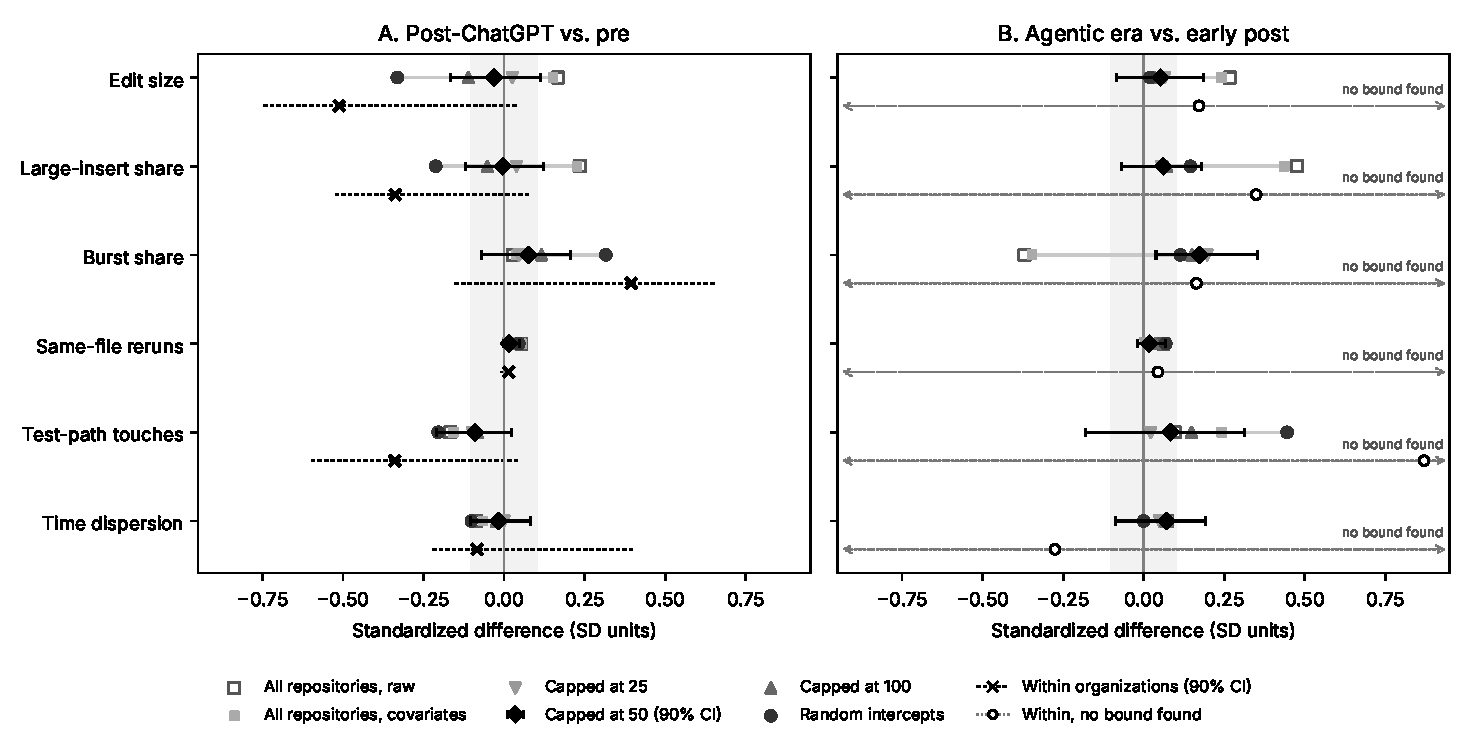
\includegraphics[width=0.98\linewidth,alt={Two panels with six signals each, showing for each signal six estimates from comparisons among all organizations joined by a line, a capped estimate with its interval, and a within-organization estimate below; in panel A edit size and large-insert share are positive for all repositories and negative under random intercepts; in panel B no within-organization bound was found within the searched range}]{figs/fig_compare_v5}
\caption{Era comparisons in standardized units (shaded band: $\pm 0.10$). A: post-ChatGPT versus pre. B: agentic era versus early post. For each signal the gray line joins the raw all-repository difference (open square), the covariate-adjusted all-repository difference (small square), the capped estimates at 25 (down triangle), 50 (diamond, with 90\% bootstrap interval), and 100 repositories (up triangle), and organization random intercepts (circle). Below each signal: the within-organization estimate on the organizations observed in both periods, with its 90\% interval (cross and dashed line) or, where the test inversion found no bound within the searched range, a hollow circle on a dotted line with arrows and the label ``no bound found''.}
\Description{Two panels listing six signals. For each signal, estimates from six comparisons among all organizations are plotted on a horizontal standardized-difference axis and joined by a line, with a within-organization estimate below. In panel A, edit size and large-insert share are about plus 0.2 for all repositories and minus 0.33 and minus 0.21 under random intercepts, with capped estimates near zero; within-organization intervals are wide. In panel B, burst share is negative for all repositories and positive under capping and random intercepts, and every within-organization estimate is marked as having no bound found.}
\label{fig:compare}
\end{figure}

\subsection{Post-ChatGPT versus pre-ChatGPT}
\label{sec:results-era}

\textit{All repositories.} Post-ChatGPT repositories in the record have larger commits ($d = $ \R{era.raw.edit}), more large insertions (\R{era.raw.large}), and fewer commits touching test paths (\R{era.raw.test}) than pre-ChatGPT repositories; the other differences are smaller than 0.1 in absolute value. Adding the covariates without an organization term changes none of these three by more than 0.02.

\textit{Contributions capped.} With no organization contributing more than $k$ repositories, the commit-size differences shrink and their sign depends on $k$: edit size is \R{era.cap25.edit}, \R{era.cap50.edit}, and \R{era.cap100.edit} at caps of 25, 50, and 100, and large-insert share \R{era.cap25.large}, \R{era.cap50.large}, and \R{era.cap100.large}. Test-path touches stay lower (\R{era.capmin.test} to \R{era.capmax.test}) and burst share higher (\R{era.capmin.burst} to \R{era.capmax.burst}), but every interval at the cap of 50 includes zero. Back-transformed from the log scale at that cap, the edit-size coefficient corresponds to a value of one plus the median lines per commit that is \R{era.natabs.edit} lower after ChatGPT (90\% CI from \R{era.natloabs.edit} lower to \R{era.nathiabs.edit} higher; Table~\ref{tab:natural}), and test-path touches are \R{era.natabs.test} percentage points lower (\R{era.natci.test}, on unadjusted means of \R{era.mean0.test} and \R{era.mean1.test}).

\textit{Random intercepts.} With organization random intercepts on all repositories, the commit-size differences reverse (\R{era.ri.edit} and \R{era.ri.large}), burst share is higher (\R{era.ri.burst}), and test-path touches (\R{era.ri.test}) and time dispersion (\R{era.ri.time}) are lower; all five survive Holm correction. All five are largely the largest organization's: without it the estimates are \R{era.loo.edit}, \R{era.loo.large}, \R{era.loo.burst}, \R{era.loo.test}, and \R{era.loo.time}.

\textit{Within organizations.} In the 14 organizations observed in both eras, no within-organization difference is distinguishable from zero (wild-bootstrap $p$ from \R{era.wpmin} to \R{era.wpmax}). The intervals contain both no difference and differences of 0.3 SD or more for five of the six signals (for edit size, \R{era.w.edit} with 90\% interval \R{era.wci.edit}; for burst share, \R{era.w.burst}, \R{era.wci.burst}). This comparison neither supports nor contradicts the comparisons among all organizations, and its non-significance is not evidence that nothing changed in those organizations.

Taken together, no signal differs in the same direction with an interval that excludes zero across the comparisons. The commit-size signals, which record how much code a commit adds at once, are larger when every repository counts once, smaller when the largest organization carries the weight, and indistinguishable from zero, with a sign that depends on the cap, when contributions are limited. Nor did commit size change once, at the boundary. Under both estimators edit size is highest for repositories begun in 2022, falls in 2023 (capped 2023-versus-2022 contrast for edit size \R{year.cap.c2322.edit}, 90\% CI \R{year.cap.c2322ci.edit}), and rises again from 2024 (Appendix Figure~\ref{fig:yearfe}), so a single post-ChatGPT coefficient averages a dip and a recovery.

\subsection{Restricting the comparison with respect to the platform change}
\label{sec:restricted}

The post-ChatGPT era includes repositories created after the platform change. Keeping post-era repositories only if they were created before the general release of fork-based creation in July 2024 (\R{preswitch.n} repositories, \R{preswitch.orgs} organizations) leaves the pre era intact and removes the post-switch record (Appendix Table~\ref{tab:regime}). The all-repository commit-size differences become small (\R{preswitch.raw.edit} and \R{preswitch.raw.large}), while the capped estimates become more negative as the cap rises (edit size \R{preswitch.cap25.edit}, \R{preswitch.cap50.edit}, \R{preswitch.cap100.edit}; large-insert share \R{preswitch.cap25.large}, \R{preswitch.cap50.large}, \R{preswitch.cap100.large}) and the random-intercept estimates more negative still (\R{preswitch.ri.edit} and \R{preswitch.ri.large}). Keeping only post-era repositories created before the fork-based beta of January 2024 (\R{prebeta.n} repositories, \R{prebeta.orgs} organizations), the all-repository differences are positive (\R{prebeta.raw.edit} and \R{prebeta.raw.large}), the capped ones negative (\R{prebeta.cap50.edit}, 90\% CI \R{prebeta.cap50ci.edit}, and \R{prebeta.cap50.large}, \R{prebeta.cap50ci.large}, at the cap of 50), and the random-intercept ones \R{prebeta.ri.edit} and \R{prebeta.ri.large}. Restricting the record does not settle the direction of the commit-size difference: in both restrictions the all-repository and random-intercept estimates keep opposite signs, and the gap between them is about as large as in the full comparison (edit size) or narrower (large-insert share) under the first restriction and wider under the second. Test-path touches are lower and burst share higher in both restrictions under most comparisons, with capped intervals that include zero.

\subsection{Repositories with one or two classified commits}
\label{sec:lowcommit}

If students had begun pasting a generated solution and committing once, the change would appear in the repositories with one or two classified commits, which the inclusion rule removes. There are \R{low.n} such repositories outside test organizations, copies, and the buffer month (\R{low.pre} pre, \R{low.post} post; \R{low.orgs} organizations), on which edit size, large-insert share, the log of the largest single insertion, and test-path touches can be computed; because these signals come from one or two commits, they are standardized by their SD in this sample rather than in the primary sample. Across all repositories, large-insert share is higher after ChatGPT ($d = $ \R{low.raw.large}; \R{low.mean0.large} to \R{low.mean1.large} of commits), edit size and the largest insertion differ little (\R{low.raw.edit}, \R{low.raw.maxins}), and test-path touches are lower (\R{low.raw.test}; \R{low.mean0.test} to \R{low.mean1.test}). With organization random intercepts all four are lower after ChatGPT (\R{low.ri.edit}, \R{low.ri.large}, \R{low.ri.maxins}, \R{low.ri.test}), and with contributions capped at 50 they are lower but with intervals that include zero or nearly do (edit size \R{low.cap50.edit}, \R{low.cap50ci.edit}; large-insert share \R{low.cap50.large}, \R{low.cap50ci.large}, whose 95\% interval \R{low.cap50ci95.large} includes zero; largest insertion \R{low.cap50.maxins}, \R{low.cap50ci.maxins}), except test-path touches (\R{low.cap50.test}, \R{low.cap50ci.test}). The all-repository increase in large insertions does not survive limiting organizations' contributions, and the record of these repositories says nothing about the repositories with no classified commit, whose share varies with record generation (Section~\ref{sec:platform}).

\subsection{The agentic era}
\label{sec:results-agent}

The agentic period lies entirely after the platform change, while most early-post repositories were created before it (Section~\ref{sec:platform}). \textit{All repositories:} agentic-era repositories have larger commits (\R{agent.raw.edit}), more large insertions (\R{agent.raw.large}), and fewer commits in bursts (\R{agent.raw.burst}). \textit{Contributions capped:} the commit-size differences shrink to between \R{agent.capmin.size} and \R{agent.capmax.size} with intervals that include zero, and burst share reverses, higher at every cap (\R{agent.cap25.burst}, \R{agent.cap50.burst}, \R{agent.cap100.burst}) with 90\% intervals that exclude zero (at the cap of 100 the 95\% interval, \R{agent.cap100ci95.burst}, includes zero). In natural units at the cap of 50 the burst difference is \R{agent.nat.burst} percentage points (\R{agent.natci.burst}), while the unadjusted means go the other way (\R{agent.mean0.burst} early post, \R{agent.mean1.burst} agentic). \textit{Random intercepts:} test-path touches are higher (\R{agent.ri.test}, Holm-corrected $p$ \R{agent.riholm.test}), but without the largest organization, which holds 542 of the 600 repositories observed on both sides of the boundary, the estimate is \R{agent.loo.test}. \textit{Within organizations:} with six organizations, the test inversion found no bound for any signal within the searched range of 50 bootstrap standard errors on each side of the estimate (for edit size, \R{agent.wrange.edit} SD), so this comparison is uninformative.

Restricting both periods to repositories without a Classroom-bot root commit of 20 or more lines, the kind whose student repositories remained collectable after the change (\R{nostarter.n} repositories, \R{nostarter.orgs} organizations), leaves burst share higher under every cap (\R{nostarter.cap25.burst}, \R{nostarter.cap50.burst}, \R{nostarter.cap100.burst}, intervals excluding zero) and under random intercepts (\R{nostarter.ri.burst}) and lower in the all-repository comparison (\R{nostarter.raw.burst}). In this restricted record, edit size and large-insert share are larger in the agentic era in every comparison among all organizations: by \R{nostarter.raw.edit} and \R{nostarter.raw.large} for all repositories, \R{nostarter.ri.edit} and \R{nostarter.ri.large} under random intercepts ($p = $ \R{nostarter.rip.edit} and \R{nostarter.rip.large} before correction), and \R{nostarter.capmin.size} to \R{nostarter.capmax.size} under the caps, with intervals that include zero (Appendix Table~\ref{tab:regime}). The direction of the burst-share difference therefore depends on whether every repository counts once or organizations are taken into account, by the cap or by random intercepts, in the full and in the restricted record.

\subsection{What else changes the answer}
\label{sec:robust}

Varying the burst window (15 or 60 minutes), the rerun length (two or four commits), and the insertion threshold (500 lines, or the largest single insertion) changes some estimates, and a few change sign (same-file reruns at four commits, under random intercepts in both contrasts and under the cap in the agentic era, and large insertions of 500 lines in the agentic era), but no variant adds clear evidence that would change the conclusions: the capped burst-share difference in the agentic era is positive with an interval excluding zero at all three windows, and no other capped interval of these variants excludes zero (Appendix Table~\ref{tab:sens}). Two choices do change answers. The strict attribution rule changes several (Section~\ref{sec:samplechange}). And in the full frame, which is mostly not coursework (\R{ff.n} repositories in \R{ff.orgs} organizations in the era contrast), commit size is larger after ChatGPT under the cap of 50 (\R{samp-full_frame_ge3.era.cap50.edit} and \R{samp-full_frame_ge3.era.cap50.large}) and under random intercepts (\R{samp-full_frame_ge3.era.ri.edit} and \R{samp-full_frame_ge3.era.ri.large}), and in the agentic era (\R{samp-full_frame_ge3.agent.cap50.edit} and \R{samp-full_frame_ge3.agent.cap50.large}; \R{samp-full_frame_ge3.agent.ri.edit} and \R{samp-full_frame_ge3.agent.ri.large}), with intervals excluding zero. The cap binds in that frame, too: the largest organization contributes \R{ff.maxorg} repositories, \R{ff.orgsover50} organizations contribute more than 50, and a cap of 50 removes \R{ff.removed50} repositories; the direction of the commit-size differences was the same with the cap as under random intercepts.
\section{Discussion}
\label{sec:discussion}

\subsection{What the comparison shows}

The differences between the commit records of the two eras depended on which commits were attributed to students, on which repositories the platform and the collector had produced in each period, and on how organizations were weighted, and none of the six signals differed in the same direction, with an interval excluding zero, across the comparisons. Commit size was larger when every repository counted once, smaller when the largest organization carried the weight, and near zero, with a sign that depended on the cap, when contributions were limited; restricting the post era to repositories created before the full switch to fork-based creation, or before its beta, did not close that gap. In the agentic era, the one difference that the capped comparison distinguished from zero, higher burst share, was reversed in the all-repository comparison. These are not findings of stability. The within-organization comparison, the closest the data come to change in a fixed setting, rested on 14 organizations for the ChatGPT boundary and 6 for the agentic one, dominated by one or two; for five of the six signals at the ChatGPT boundary its intervals contained both no change and changes of 0.3 SD or more, and for the agentic boundary no bound was found within the searched range. The comparisons among all organizations describe the repositories of the record, and that record changed in what it contained. None of this makes agreement across every comparison the condition for a meaningful result: the comparisons answer different questions, and a difference that holds under one weighting but not another is informative about which organizations carry it. What it requires is that a study say which comparison it reports and what that comparison weights.

The strongest finding is therefore about the record rather than about students. A platform change that had nothing to do with students, combined with a collection rule that is the default of the search interface, removed most starter-code assignments from what could be collected after mid-2024 and added instructors' copies to it. A study that compared the record across 2024 without checking how it was generated would compare different kinds of assignments and would count instructors' repositories as students'. Activity attribution and organization weighting then determine how much of the remaining difference is attributed to students and to which organizations.

\subsection{What other studies should check}

Table~\ref{tab:diagnostics} condenses the checks into a diagnostic for studies that compare courses, cohorts, or organizations across a calendar boundary using repository data. Each row names the information used here and what goes wrong if the check is omitted, with this corpus's example. None of the checks requires data beyond what a collector already has or can read in the platform's documentation: commit and repository timestamps, author identifiers and repository names, the name structure and fork relations of repositories, the platform's changelog, and the number of repositories per organization.

\begin{table}
\caption{Diagnostics for comparing educational repository records across periods, organized by the three checks. Example: what the omission did, or would have done, in this corpus.}
\label{tab:diagnostics}
\scriptsize
\setlength{\tabcolsep}{3pt}
\begin{tabular}{@{}>{\raggedright\arraybackslash}p{2.5cm} >{\raggedright\arraybackslash}p{3.6cm} >{\raggedright\arraybackslash}p{6.4cm}@{}}
\toprule
Check & Information used & If omitted (example from this corpus) \\
\midrule
\multicolumn{3}{@{}l}{\textit{Activity attribution}} \\
Pre-existing history & Commit time against repository creation & Template and earlier-project history counted as student work (5.8\% of commits kept by the previous rule, 14.8\% in the pre era, predated the repository by more than a day) \\
Shared commits & SHA sharing and timing & Teammates' and students' own pushes excluded as templates (12\% of the previous rule's inherited commits postdated the repository) \\
Authors in many repositories & Owner match and author breadth & Students in team courses excluded as staff (\R{staff.narrow.S} of \R{staff.narrow.n} reviewed commits by authors in 5 to 49 repositories), or instructors kept \\
Status of the check & What evidence the review uses beyond the rule's inputs & A metadata-based review read as validated accuracy \\
\midrule
\multicolumn{3}{@{}l}{\textit{Record generation and collection}} \\
Platform's creation method & Changelog and documentation; root commits, name structure, and fork relations by creation date & Assignments with starter code missing after mid-2024 (starter share from 68--95\% per half-year in 2021 to mid-2024 to 5--33\% after); instructors' copies counted as student repositories (52--68\% of verified repositories per half-year) \\
Collector's rule & Whether the search returns forks, private or empty repositories & Fork-created student repositories invisible without notice \\
Observation window & Time from creation to collection & Recent repositories' lack of commits read as non-participation \\
\midrule
\multicolumn{3}{@{}l}{\textit{Organization weighting}} \\
Composition & All-repository, covariate-adjusted, capped, and random-intercept comparisons side by side & One weighting reported as the answer (edit size \R{era.raw.edit} for all repositories, \R{era.ri.edit} under random intercepts) \\
Dominant organizations & Leave-one-out; cluster sizes & One organization's change reported as everyone's (random-intercept edit size \R{era.ri.edit}, \R{era.loo.edit} without the largest organization) \\
Few clusters & Wild cluster bootstrap with test inversion; the searched range reported when no bound is found & False precision, or a non-significant result read as no change (6 organizations, one with 542 of 600 repositories) \\
Standardization & Raw against within-group standardized contrasts & A null by construction (the registered analysis standardized within organization-by-era cells; Appendix~\ref{app:registered}) \\
\bottomrule
\end{tabular}
\end{table}

Two of the rows deserve emphasis. First, the status of an attribution check depends on its evidence: a review that reads the same metadata the rule uses, plus subject lines, can find a rule's clear errors, as it did here, but cannot certify that a commit is a student's work on the assignment; a more independent check is described under future work. Second, the platform's history is part of the data. Commit records from hosted platforms are produced by software that changes, and the change in 2024 was announced and documented; it became a threat to the comparison only because the collection rule interacted with it.

\subsection{Implications for teaching and assessment}

For instructors, the practical conclusion concerns what commit records need to be combined with, not whether they are useful. This study did not compare commit patterns with students' actual AI use or understanding, so its signals give no basis for judging whether an individual student used AI or understood the committed code. Commit histories remain useful records of how work was organized over time, and process requirements stated in terms of them (frequent commits, incremental work, contact with tests) remain requirements about the shape of a history. Where an instructor wants evidence about tool use or understanding, the record needs to be joined with data that address that question directly, such as IDE or autograder logs, explanation or reflection tasks, or conversation about the work, and any indicator built from commit histories needs to be validated against such data before it is used to judge students.

\subsection{Limitations}
\label{sec:limitations}

The design is observational: nothing was manipulated, eras are compared across different organizations, and the within-organization evidence rests on 14 and 6 organizations dominated by one or two. The attribution review is metadata-based, small, and clustered, and its judgments were made by a language model and checked by the author; it indicates the kinds of the rule's errors rather than their precise rates, and team repositories are classified by elimination. Message distinctiveness could not be recomputed on classified commits and is reported only as a supplementary result. The restricted comparisons remove the record after the general release of fork-based creation, but not the beta period before it with certainty, and they cannot recover the repositories that left the record. The sample is public Classroom coursework, which instructors chose to run publicly, and its organizations are unequal in size and in kind; verification establishes a Classroom repository, not a novice or an introductory course. The signals read process at commit grain and cannot see what happened between commits or whether a student understood a change. There are no learning outcomes in the data, and silent AI use is invisible. The analyses are exploratory, specified after earlier analyses of the same data had failed. Because Classroom no longer creates repositories, the record cannot be extended to later cohorts.

\subsection{Future work}

Three studies follow. A check of activity attribution on a sample of commits that uses the code changed and the assignment descriptions and is carried out by a reviewer blind to the rule's verdict would give a more independent basis for estimating the rule's accuracy than the metadata-based review reported here, though its judgments would still not be ground truth. A within-course design, in which the same assignments are run across years and students report their tool use, would hold the course fixed by design rather than by estimation and relate commit-level differences to reported use. And the signals could be validated one at a time against IDE-level process data in a course that records both.

\section{Conclusion}
\label{sec:conclusion}

A public educational repository is a record produced by a platform, selected by a collector, and supplied unequally by organizations, before it is a trace of students' work. In GitHub Classroom coursework collected shortly before the platform's retirement, a 2024 change in how Classroom created repositories, together with a search that does not return forks, removed most starter-code assignments from the collectable record and added instructors' copies to it; rules that attribute commits to students erred in both directions; and the answer to an era comparison depended on how organizations were weighted. Once these were taken into account, no commit-stream signal differed in the same direction, with an interval excluding zero, across comparisons between the eras before and after generative AI, and the organizations observed in both periods were too few to show either change or its absence. The difference between eras in such a record cannot be read as a change in students' behavior until the record's sources, its generation and collection, and the organizations' contributions have been checked. Those checks are necessary for reading commits as learning; whether commit patterns reflect learning or understanding has to be established, beyond them, against evidence the commit record does not contain.

\section*{Data and Materials Availability}
The collection, extraction, and analysis scripts, the derived tables with hashed identifiers, the result files of every analysis, the registered protocol and its results, the decision log, and the generative-AI use log are available in a public repository archived with a DOI, which is withheld for review; an anonymized copy of the repository is available at \url{https://anonymous.4open.science/r/commit-record-checks-B7E2}. From the distributed files alone, the package's entry point rebuilds the generated tables, the numbers cited in the text, and the four figures from the result files and compares them with the submitted ones; re-fits, on request, the models of the era and agentic-era contrasts, of their restricted, threshold, year, low-commit, and sample variants, and of the attribution-rule variants from the derived tables and compares every re-fitted number with the distributed results; and checks each number typed into the manuscript source against the result files and derived tables where it can be computed from them, listing the others as design constants, dates, or recorded values. The check of the random-intercept implementation (Appendix~\ref{app:estimation}), the trailer model (Appendix~\ref{app:trailers}), and the tabulation behind Table~\ref{tab:recordgen} are distributed as scripts and results and are not re-run by the entry point. Collection, extraction, owner matching, assignment-copy detection, and the commit review need the raw commit logs or the access-controlled review file and cannot be run from the package; their outputs are distributed. The registered analysis and the intermediate analyses of Appendix~\ref{app:history} are distributed as recorded results and are not re-run by the entry point. Raw commit logs and the review file, which contain names, e-mail addresses, and commit subjects, are available to reviewers on request under access control. The CodeWorkout data used in Appendix~\ref{app:registered} are the Spring 2019 and Fall 2019 ProgSnap2 release files of the 2nd CSEDM Data Challenge named there, both distributed with PSLC DataShop dataset 3458 \citep{codeworkout2020dataset}, which requires a free DataShop account.

\section*{Generative AI Disclosure}
In accordance with the ACM Policy on Authorship, I disclose that a large language model (Claude, Anthropic: Claude Fable 5.1 and Claude Opus 5.5 for the October 2026 analyses and manuscript, Claude Fable 5 for the August 2026 collection and registered analysis) was used under my direction to draft collection and analysis code from written specifications and run it, to make the first judgments of the review of sampled commits under a written protocol (I checked them), to audit code, numbers, claims, and references in separate sessions, and to draft and edit the prose of this manuscript. My review memos on drafts were prepared with the assistance of a second language model (ChatGPT Codex, OpenAI), and every claim in them was checked against the data before it was acted on. All research questions, definitions, modeling decisions, interpretations, and final wording are my own; all code was reviewed by me; and every reference was checked against the publisher's record or the cited source itself.

\appendix


\section{The Registered Analysis as Specified}
\label{app:registered}

\textit{Registration.} Open Science Framework, August 6, 2026, secondary-data preregistration after collection and before outcome computation. The OSF link is withheld for review; the registered protocol, its frozen SHA-256 manifest, and the registered results are in the folder \texttt{registration} of the anonymized repository (see Data and Materials Availability). \textit{Registered sample.} All repositories in the frame with at least five commits by at least one non-bot author (25,743), of which 22,071 had at least five defined signals (8,740 pre, 13,198 post, 552 with AI trailers). \textit{Registered signals.} The six of Table~\ref{tab:signals} and message distinctiveness (Appendix~\ref{app:msg}), computed on all non-bot commits, with the large-paste signal defined by the era-by-language 95th percentile, plus AI-paste co-occurrence. \textit{Registered standardization.} Within student for students with two or more repositories (29\% of the sample), within organization-by-era cohort otherwise (71\%), with an era-level fallback for cohorts of fewer than five repositories. \textit{Registered composite.} Sign-aligned equal-weight mean, negated as the shortcut composite. \textit{Registered models.} Linear mixed models of the composite on the label, log commit count, author count, and language family with organization random intercepts; within-organization permutation tests (10,000); Holm correction over four confirmatory tests (H1, H2a, H3, H5; the registration's H2b, a within-student trailer comparison on 77 students, was registered for direction only, and H4, a process-outcome dissociation using continuous-integration outcomes, was registered as exploratory and conditional on data that the collection did not obtain); equivalence margin $d = \pm 0.10$; placebos P1 (fake boundary at June 1, 2021) and P2 (\textit{Signed-off-by}). Table~\ref{tab:registered} gives the confirmatory results as the registered scripts produced them.

\begin{table}[!htbp]
\caption{Registered confirmatory results, as produced by the registered scripts.}
\label{tab:registered}
\footnotesize
\setlength{\tabcolsep}{4pt}
\begin{tabular}{@{}>{\raggedright\arraybackslash}p{2.3cm} >{\raggedright\arraybackslash}p{1.3cm} >{\raggedright\arraybackslash}p{4.6cm} >{\raggedright\arraybackslash}p{2.8cm} >{\raggedright\arraybackslash}p{1.6cm}@{}}
\toprule
Test & Effect & Statistics & Placebo & Registered verdict \\
\midrule
H1 era shift (composite) & $d = -0.027$ & 90\% CI $[-0.050, -0.004]$; $p_{\text{Holm}} = .17$; perm $p = .23$; 43 robustness specifications in $[-0.056, 0.013]$ & P1 passed ($d = 0.001$, $p = .98$) & Equivalent \\
H2a AI trailer (composite) & $d = 0.298$ & $p_{\text{Holm}} = 1.2 \times 10^{-4}$; perm $p = .004$; $n = 1{,}276$ & P2 failed ($d = 0.158$, $p = .016$; $n = 1{,}565$) & Confounded \\
H3 widening gap & $\beta = 0.025$ & $p = .52$; 2,124 students, 4,669 later repositories; baseline $\times$ trailer $\beta = +0.20$, $p = .03$ (opposite direction) & & Not supported \\
H5 convergent validity & $r = -0.05$ & 95\% CI $[-0.12, 0.01]$; Spearman $\rho = -0.10$; $n = 916$ CodeWorkout students; threshold $r \geq .30$ & & Not supported \\
\bottomrule
\end{tabular}
\end{table}

\textit{Diagnosis.} Standardizing a signal within an organization-by-era cell sets its mean to zero in that cell, so the pre and post cells of every organization have identical means on every signal and a between-era contrast is zero by construction, just as centering a predictor within clusters removes all of its between-cluster variation \citep{enders2007centering}. The registered analysis standardized 71\% of its sample this way and concluded equivalence within $d = \pm 0.10$; on the raw scale the same signals in the same sample differed between eras by up to $0.26$ standard deviations (Figure~\ref{fig:registered}). The 95th-percentile definition of a large paste had a related defect: it classified 5\% of commits as large in every era by construction.

\begin{figure}[!htbp]
\centering
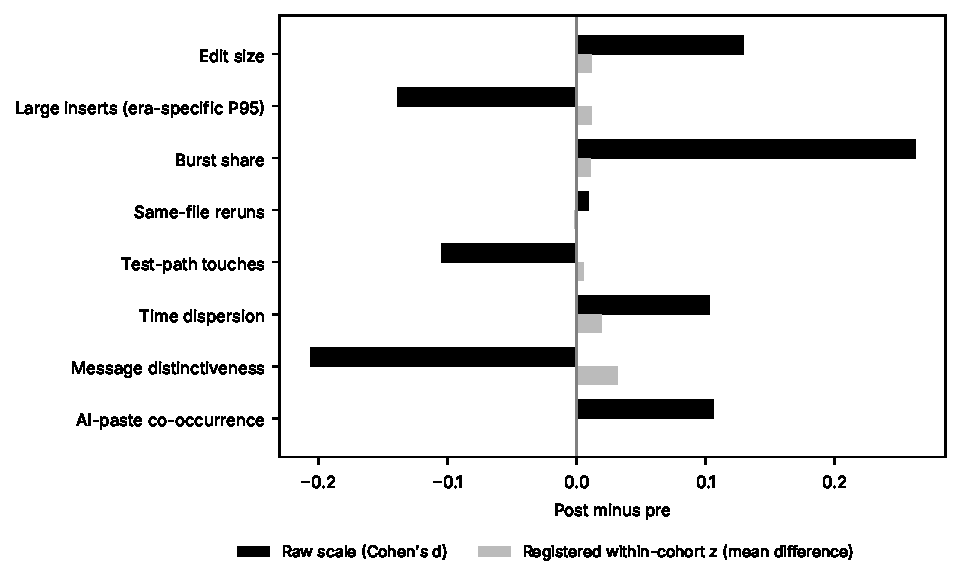
\includegraphics[width=0.75\linewidth,alt={Bar chart of eight signals comparing raw-scale era differences, which range from minus 0.21 to plus 0.26, with registered within-cohort standardized differences, which are all near zero}]{figs/fig_registered_vs_raw_v3}
\caption{Within-cohort standardization in the registered analysis. For the eight registered signals in the registered sample (22,071 repositories, 71\% standardized within organization-by-era cohort), the raw-scale standardized difference between eras (black) and the difference after the registered standardization (gray).}
\Description{Horizontal bar chart with eight signal rows. Black bars show raw-scale post-minus-pre differences ranging from about minus 0.21 to plus 0.26; gray bars show registered-standardization differences all within plus or minus 0.04.}
\label{fig:registered}
\end{figure}

\textit{Estimation.} The registered models were fitted with statsmodels' default L-BFGS optimizer, which this study later found to return, for the random-intercept models of the reported analysis, the coefficients of the fixed-effects solution under the label of a random-intercept fit (Appendix~\ref{app:estimation}); the registered fits were not re-examined, and the registered results are reported as the registered scripts produced them.

\textit{H1 and H2a.} The H1 null was produced by the registered standardization (Figure~\ref{fig:registered}). H2a was not removed by it, because trailer status varies within organization-by-era cells; the registered version read this asymmetry as evidence of a sensitive instrument, which it was not.

\textit{H3.} The registered moderation test asked whether a student's baseline composite in a first repository moderated the era effect in later repositories; the registered prediction was a negative interaction of the baseline with era and with trailer status (a widening gap). The era interaction was null. The trailer interaction, in the same model, was positive at $p = .03$ uncorrected, the opposite of the registered direction; it would not survive Holm correction over the four confirmatory tests, it was computed on the cohort-standardized composite that Figure~\ref{fig:registered} shows to be uninformative, and in the verified Classroom sample only 35 students have repositories in both eras. It is reported as registered and is not re-run, and the paper makes no claim about moderation in either direction.

\textit{H5.} Commit-analog indicators (edit-size deltas between code states, submission bursts, same-problem retry arcs, temporal dispersion) were computed from the CodeWorkout session logs of Spring and Fall 2019 in the ProgSnap2 format (release files \texttt{S19\_\allowbreak All\_\allowbreak Release\_\allowbreak 2\_10\_22.zip} and \texttt{F19\_\allowbreak Release\_\allowbreak All\_\allowbreak 05\_23\_22.zip}, the full-data releases of the 2nd CSEDM Data Challenge, both distributed with PSLC DataShop dataset 3458 \citep{codeworkout2020dataset}; 916 students) and correlated with the datasets' native error and resubmission indicators. CodeWorkout was chosen because it is a large public ProgSnap2 dataset of CS1 submissions with per-attempt error and score events and because it predates generative AI. The pooled correlation was $r = -0.05$ (F19: $-0.03$; S19: $-0.02$; timing-only variant $0.12$). The composite does not measure what autograder struggle indicators measure; whether individual signals would is untested.

\FloatBarrier
\section{Decisions and Analysis History}
\label{app:history}
\label{app:decisions}

\textit{Decisions.} The registered implementation decisions D1 to D10 and the post-registration decisions E1 to E15, each with its date, rationale, and implementing script, are listed in the decision log of the replication package; D1, D2, D4, D5, and D6 (bot-commit exclusion, merge-commit exclusion from line-based signals, trailer-line stripping before message embedding, domain restrictions for distinctiveness and dispersion, cohort fallbacks) carry over. The post-registration decisions that shape the reported results fall into four groups.
\textit{Scales and estimands} (E1, E2, E3, E5, E11, E15): raw scales instead of within-group standardization, absolute large-insert thresholds, no composite and no AI-paste co-occurrence signal, comparisons named by what they estimate with effects also in natural units, and one standardization denominator per contrast and signal (the SD in the primary sample of the contrast), so that differences between comparisons are not differences in denominators.
\textit{Sample and attribution} (E4, E9, E10, E14): verified Classroom repositories outside test organizations; signals computed on commits attributed to students under the rule of Section~\ref{sec:attribution}, with the previous rule and six variants as sensitivity analyses; a separate analysis of one- and two-commit repositories; exclusion of Classroom's per-assignment copies; and the comparisons restricted with respect to the platform change.
\textit{Estimation and inference} (E7, E8, E12, E13, E14): several estimators side by side with leave-out checks and caps of 25, 50, and 100; an independent restricted maximum likelihood implementation; organization-bootstrap intervals for the capped comparison; a wild cluster bootstrap with test inversion for the within-organization comparison, reporting the searched range when no bound is found; and estimates and intervals reported across comparisons instead of a rule requiring every comparison to agree.
\textit{Supplementary analyses} (E6, E14, E15): the human co-author placebo tested as a difference within one model; message distinctiveness removed from the comparisons; design-based estimates for the review of staff-like exclusions.
The large-insert thresholds that the registered definition would produce for the primary sample (95th percentile of added lines in the pre era, by language family) are: C/C++ 256,181; C\# 40,880; other 17,325; web markup 9,287; notebooks 2,397; JavaScript/TypeScript 2,252; Java/Kotlin 358; Python 214; all languages 28,622.

\textit{History.} Four analyses preceded the one reported here; the decision log describes each. The \textit{registered analysis} (August 2026) concluded equivalence from a within-cohort-standardized composite (Appendix~\ref{app:registered}). The \textit{first two corrections} (October 2026) analyzed all non-bot commits of verified repositories and fitted their mixed models with statsmodels' default L-BFGS optimizer, which on these data returned the coefficients of the fixed-effects solution under the label of a random-intercept fit (Appendix~\ref{app:estimation}); the era differences they reported changed or reversed when the largest organization was removed and did not survive a wild cluster bootstrap. The \textit{third correction} computed the signals on commits attributed by the previous rule and refitted the models with a checked optimizer after separate audits; its findings on message distinctiveness and on the largest insertion in one- and two-commit repositories did not survive the checks of the attribution rules, the exclusion of Classroom's copies, and organization-bootstrap intervals. The checks that this paper reports (the attribution rules, Classroom's 2024 change and the copies in the record, and the dependence on organization weighting) came out of the review of that version.
\FloatBarrier
\section{Estimation Details}
\label{app:estimation}

\textit{Capped comparison.} The capped estimate is the mean of the random-intercept coefficient over 200 independent draws of at most $k$ repositories per organization. Its interval comes from an organization-level cluster bootstrap \citep{cameron2008bootstrap, cameron2015practitioner}: in each of 1,000 replicates, organizations are drawn with replacement, each drawn copy is treated as a distinct organization, the capped estimator is applied with five draws, and the replicate's estimate is the mean over the five; the 90\% and 95\% intervals are percentiles of the replicates. The organization is resampled because it is the unit whose presence in the record is random from the point of view of the analysis and within which repositories are dependent. Each replicate carries one fifth of the between-draw variance, against one two-hundredth in the point estimate, so the intervals are slightly conservative; removing this excess would narrow them by less than 4\% for five signals and by about a fifth (18\% and 21\% in the two contrasts) for same-file reruns, whose draws vary most. Standardized and natural-unit estimates come from the same fits and replicates ($d = \hat\beta / s$, with $s$ the standard deviation of the signal in the primary analysis sample of the contrast, the denominator used for every comparison of that contrast). Sensitivity analyses and year effects use 500 replicates.

\textit{Standardization.} An earlier version divided each comparison by the SD of the signal in the sample on which that comparison was fitted (for example, the spanning organizations for the within-organization comparison, or the sample without the largest organization for the leave-out estimate). The estimates reported here use one denominator per contrast and signal (Section~\ref{sec:estimands}). They were re-expressed exactly, as $d = \hat\beta / s$: the deterministic coefficients (raw differences, random-intercept, leave-out, and within-organization point estimates) were recomputed from the derived data and matched the stored ones in all 224 checks, and the bootstrap and test-inversion intervals were rescaled from the stored ones rather than re-run. The changes are largest where a comparison's sample differs most from the primary sample: the within-organization comparisons, whose spanning organizations have SDs between 0.38 and 1.27 times those of the primary samples (for edit size after ChatGPT, \R{era.w.edit} instead of $-0.42$), and the restricted comparisons (for edit size in the agentic era without platform-copied starter code, \R{nostarter.raw.edit} instead of $+0.70$ for all repositories).

\textit{Stability.} Table~\ref{tab:stability} compares the reported capped estimates with estimates from 1,000 draws and with a complete repetition of the procedure on a new random stream. The estimates differ by at most 0.009 SD and the interval endpoints by at most 0.015; the differences are small and do not change any interpretation in the text. An earlier version combined the variance across draws with an approximation to the rule for multiply imputed estimates \citep{rubin1987imputation} (the within-draw variance taken as the square of the mean standard error rather than the mean squared standard error), which assumes that each draw is a completed data set and has no claim to coverage for subsamples of one record. It is shown in the table for comparison only; the text uses the bootstrap throughout.

\begin{table}[h]
\caption{Stability of the capped estimate (cap 50): reported estimate (200 draws), estimate from 1,000 draws, and a repetition of the whole procedure with a new random stream; 90\% organization-bootstrap intervals as reported and in the repetition; for comparison only, the interval from the multiple-imputation combining rule; and the between-draw standard deviation relative to the bootstrap standard error.}
\label{tab:stability}
\scriptsize
\setlength{\tabcolsep}{2.5pt}
\begin{tabular}{@{}l r r r l l l r@{}}
\toprule
Signal & $d$ & $d_{1000}$ & Rep. & Bootstrap & Bootstrap, rep. & Rubin & $s_{\text{draw}}/s_{\text{boot}}$ \\
\midrule
\multicolumn{8}{@{}l}{Post-ChatGPT $-$ pre} \\
\midrule
Edit size & $-0.03$ & $-0.04$ & $-0.03$ & $[-0.17, +0.11]$ & $[-0.17, +0.12]$ & $[-0.15, +0.09]$ & 0.58 \\
Large-insert share & $0.00$ & $0.00$ & $0.00$ & $[-0.12, +0.12]$ & $[-0.11, +0.11]$ & $[-0.11, +0.10]$ & 0.52 \\
Burst share & $+0.08$ & $+0.08$ & $+0.08$ & $[-0.07, +0.21]$ & $[-0.06, +0.21]$ & $[-0.05, +0.21]$ & 0.49 \\
Same-file reruns & $+0.02$ & $+0.02$ & $+0.02$ & $[-0.003, +0.05]$ & $[-0.003, +0.04]$ & $[-0.03, +0.06]$ & 1.29 \\
Test-path touches & $-0.09$ & $-0.09$ & $-0.09$ & $[-0.21, +0.02]$ & $[-0.21, +0.03]$ & $[-0.21, +0.03]$ & 0.43 \\
Time dispersion & $-0.02$ & $-0.01$ & $-0.01$ & $[-0.10, +0.08]$ & $[-0.10, +0.08]$ & $[-0.12, +0.08]$ & 0.41 \\
\midrule
\multicolumn{8}{@{}l}{Agentic era $-$ early post} \\
\midrule
Edit size & $+0.05$ & $+0.05$ & $+0.05$ & $[-0.08, +0.19]$ & $[-0.10, +0.18]$ & $[-0.09, +0.20]$ & 0.33 \\
Large-insert share & $+0.06$ & $+0.06$ & $+0.06$ & $[-0.07, +0.18]$ & $[-0.07, +0.17]$ & $[-0.08, +0.20]$ & 0.36 \\
Burst share & $+0.17$ & $+0.18$ & $+0.17$ & $[+0.04, +0.35]$ & $[+0.02, +0.34]$ & $[-0.002, +0.35]$ & 0.34 \\
Same-file reruns & $+0.02$ & $+0.02$ & $+0.01$ & $[-0.02, +0.07]$ & $[-0.02, +0.07]$ & $[-0.06, +0.09]$ & 1.39 \\
Test-path touches & $+0.08$ & $+0.07$ & $+0.07$ & $[-0.18, +0.31]$ & $[-0.19, +0.31]$ & $[-0.11, +0.27]$ & 0.36 \\
Time dispersion & $+0.07$ & $+0.07$ & $+0.07$ & $[-0.09, +0.19]$ & $[-0.09, +0.19]$ & $[-0.07, +0.21]$ & 0.27 \\
\bottomrule
\end{tabular}
\end{table}


\textit{Within-organization comparison.} The model is refitted under the null, its residuals within each organization are multiplied by a common random weight, and the observed coefficient is compared with the distribution of coefficients refitted to the resulting outcomes (1,999 replicates), following the restricted wild cluster bootstrap \citep{cameron2008bootstrap, roodman2019boottest}; unlike the studentized test those authors recommend, the test compares coefficients, not $t$-statistics. The weights are Rademacher for 14 clusters and Webb's six-point distribution for 6, because Rademacher weights on 6 clusters give only $2^6 = 64$ possible bootstrap samples \citep{webb2023reworking, roodman2019boottest}. The 90\% interval contains each null value that the test does not reject at the 10\% level, over a grid that extends at least six bootstrap standard errors on each side of the estimate. For the agentic-era comparison, no value was rejected anywhere on that grid, and the inversion was repeated on a grid of 401 points extending 50 bootstrap standard errors on each side; again no value was rejected, so Table~\ref{tab:main} reports the searched range (in SD units) instead of an interval.

\textit{Random-intercept models.} The models are fitted by restricted maximum likelihood with an implementation written for this study, which profiles the likelihood over the ratio of the organization variance to the residual variance, maximizes it by a bounded scalar search, and returns the generalized-least-squares coefficients and standard errors given the estimated variance components, the convention of the R packages \texttt{lme4} and \texttt{nlme}. For the 18 random-intercept models of the two main contrasts and the low-commit analysis, it was checked against statsmodels MixedLM with the Nelder--Mead and BFGS optimizers. Against Nelder--Mead, the coefficients agree to within $7 \times 10^{-5}$, the restricted log-likelihoods to within $1.1 \times 10^{-5}$, and the organization variances to within $3.1 \times 10^{-4}$, and the implementation's log-likelihood is at least as high as every statsmodels fit; BFGS failed to converge on 3 of the 18. Statsmodels' standard errors, which come from the observed information including the variance parameters, are up to 7\% larger in 17 models and 25\% larger in one model whose organization variance is at the boundary of zero.

\textit{The optimizer failure.} With statsmodels' default L-BFGS optimizer, 15 of the same 18 models returned a fit flagged as converged with a log-likelihood of $+\infty$ and an organization variance of exactly zero, and 16 returned fixed-effect coefficients identical, to within $10^{-8}$, to those of the ordinary least-squares regression with organization fixed effects. The random-intercept model was not fitted; the optimizer stopped at an invalid point and reported, under the label of a random-intercept model, the coefficients of the fixed-effects solution. The first and second corrections of this analysis used that optimizer (Appendix~\ref{app:history}).

\FloatBarrier
\section{Additional Results}
\label{app:sens}

This appendix gives the checks of the previous attribution rule (Table~\ref{tab:activity}), the full results of the two main contrasts (Tables~\ref{tab:era} and~\ref{tab:agent}), the comparisons restricted with respect to the platform change (Table~\ref{tab:regime}), the capped estimates in natural units (Table~\ref{tab:natural}), threshold, sample, and rule variants (Tables~\ref{tab:sens} to~\ref{tab:rules}), and year-of-first-commit effects (Figure~\ref{fig:yearfe}). The text of Section~\ref{sec:comparisons} discusses the variants that change an interpretation.

\begin{table}[!htbp]
\caption{Checks of the previous attribution rule, non-bot commits in verified Classroom repositories outside test organizations. Before creation: committer timestamp earlier than the repository's creation. Owner match: author identifiers match the repository name. Review: 20 commits drawn at random from each category and judged, under a protocol similar to that of Section~\ref{sec:attribution}, as student work in the repository, pre-existing history or instructor or platform content, or undeterminable (only the counts were recorded). The review drew on an earlier tabulation of the same categories, whose sizes differ in four rows (632, 3,960, 7,335, and 65,242).}
\label{tab:activity}
\footnotesize
\setlength{\tabcolsep}{4pt}
\begin{tabular}{@{}p{5.6cm} r r r r@{}}
\toprule
Category under the previous rule & Commits & Before creation & Owner match & Review \\
\midrule
Shared SHA (``inherited''), committed before creation & 4,904 & 100\% & 4\% & 0/20/0 \\
Shared SHA (``inherited''), committed after creation & 649 & 0\% & 17\% & 16/0/4 \\
Staff-like author, owner match & 550 & 0\% & 100\% & 20/0/0 \\
Staff-like author, no owner match & 3,924 & 1\% & 0\% & 2/17/1 \\
Kept as student, committed before creation & 7,338 & 100\% & 8\% & 2/14/4 \\
Kept as student, no owner match, after creation & 65,277 & 0\% & 0\% & 17/2/1 \\
\bottomrule
\end{tabular}
\end{table}


\begin{table}[!htbp]
\caption{Post-ChatGPT minus pre-ChatGPT, full results (4,941 repositories, 391 organizations; 2,066 pre, 2,875 post). Cov.: all repositories with the covariates and no organization term. RI ($p$): organization random intercepts with the uncorrected $p$-value (the text reports Holm-corrected values where significance is claimed). Capped estimates with their 90\% organization-bootstrap intervals (1,000 replicates) on the second line. Lower part: random-intercept estimates leaving out each of the ten largest organizations (minimum and maximum) and the five largest together; within-organization comparison on the 14 organizations observed in both eras with its wild-bootstrap $p$; organization-level paired median and the number of organizations in which the post mean is higher.}
\label{tab:era}
\scriptsize
\setlength{\tabcolsep}{2.5pt}
\begin{tabular}{@{}l r r c c c r@{}}
\toprule
Signal & Raw & Cov. & Cap 25 & Cap 50 & Cap 100 & RI ($p$) \\
\midrule
Edit size & $+0.17$ & $+0.15$ & $+0.02$ & $-0.03$ & $-0.11$ & $-0.33$ ($<$.001) \\
 & & & $[-0.09, +0.14]$ & $[-0.17, +0.11]$ & $[-0.28, +0.08]$ & \\[2pt]
Large-insert share & $+0.24$ & $+0.23$ & $+0.04$ & $0.00$ & $-0.05$ & $-0.21$ ($<$.001) \\
 & & & $[-0.08, +0.14]$ & $[-0.12, +0.12]$ & $[-0.19, +0.09]$ & \\[2pt]
Burst share & $+0.03$ & $+0.04$ & $+0.05$ & $+0.08$ & $+0.12$ & $+0.32$ ($<$.001) \\
 & & & $[-0.09, +0.17]$ & $[-0.07, +0.21]$ & $[-0.03, +0.26]$ & \\[2pt]
Same-file reruns & $+0.05$ & $+0.05$ & $+0.01$ & $+0.02$ & $+0.02$ & $+0.05$ (.133) \\
 & & & $[-0.003, +0.04]$ & $[-0.003, +0.05]$ & $[-0.001, +0.06]$ & \\[2pt]
Test-path touches & $-0.17$ & $-0.16$ & $-0.10$ & $-0.09$ & $-0.08$ & $-0.20$ ($<$.001) \\
 & & & $[-0.24, +0.04]$ & $[-0.21, +0.02]$ & $[-0.23, +0.03]$ & \\[2pt]
Time dispersion & $-0.09$ & $-0.07$ & $0.00$ & $-0.02$ & $-0.02$ & $-0.10$ (.018) \\
 & & & $[-0.09, +0.10]$ & $[-0.10, +0.08]$ & $[-0.10, +0.07]$ & \\[2pt]
\bottomrule
\end{tabular}

\medskip

\begin{tabular}{@{}l l r l r l@{}}
\toprule
Signal & LOO min/max & Drop 5 & Within [90\% CI] & $p_{\text{wild}}$ & Paired median, $+/14$ \\
\midrule
Edit size & $-0.39$/$-0.03$ & $-0.03$ & $-0.51$ $[-0.75, +0.04]$ & .171 & $-0.15$, 5 \\
Large-insert share & $-0.27$/$+0.03$ & $-0.01$ & $-0.34$ $[-0.53, +0.08]$ & .269 & $-0.02$, 5 \\
Burst share & $+0.03$/$+0.39$ & $+0.07$ & $+0.39$ $[-0.15, +0.66]$ & .510 & $-0.27$, 6 \\
Same-file reruns & $+0.02$/$+0.05$ & $0.00$ & $+0.01$ $[-0.01, +0.03]$ & .380 & $0.00$, 6 \\
Test-path touches & $-0.27$/$+0.01$ & $-0.07$ & $-0.34$ $[-0.60, +0.04]$ & .330 & $0.00$, 5 \\
Time dispersion & $-0.12$/$-0.03$ & $+0.01$ & $-0.08$ $[-0.22, +0.40]$ & .940 & $+0.01$, 7 \\
\bottomrule
\end{tabular}
\end{table}

\begin{table}[h]
\caption{Agentic era (February 2025 onward) minus early post (January 2023 to January 2025), full results (2,875 repositories, 230 organizations; 1,608 early post, 1,267 agentic). Columns as in Table~\ref{tab:era}; within-organization and paired comparisons on the 6 organizations observed in both periods (600 repositories, 542 in one organization); the test inversion found no bound within the searched range (50 bootstrap standard errors on each side of the estimate).}
\label{tab:agent}
\scriptsize
\setlength{\tabcolsep}{2.5pt}
\begin{tabular}{@{}l r r c c c r@{}}
\toprule
Signal & Raw & Cov. & Cap 25 & Cap 50 & Cap 100 & RI ($p$) \\
\midrule
Edit size & $+0.27$ & $+0.24$ & $+0.06$ & $+0.05$ & $+0.03$ & $+0.02$ (.766) \\
 & & & $[-0.08, +0.20]$ & $[-0.08, +0.19]$ & $[-0.08, +0.17]$ & \\[2pt]
Large-insert share & $+0.48$ & $+0.44$ & $+0.06$ & $+0.06$ & $+0.07$ & $+0.14$ (.021) \\
 & & & $[-0.07, +0.18]$ & $[-0.07, +0.18]$ & $[-0.07, +0.19]$ & \\[2pt]
Burst share & $-0.37$ & $-0.35$ & $+0.20$ & $+0.17$ & $+0.15$ & $+0.11$ (.111) \\
 & & & $[+0.05, +0.36]$ & $[+0.04, +0.35]$ & $[+0.02, +0.33]$ & \\[2pt]
Same-file reruns & $+0.06$ & $+0.07$ & $+0.01$ & $+0.02$ & $+0.04$ & $+0.07$ (.094) \\
 & & & $[-0.02, +0.05]$ & $[-0.02, +0.07]$ & $[-0.02, +0.10]$ & \\[2pt]
Test-path touches & $+0.10$ & $+0.24$ & $+0.02$ & $+0.08$ & $+0.15$ & $+0.45$ ($<$.001) \\
 & & & $[-0.19, +0.23]$ & $[-0.18, +0.31]$ & $[-0.20, +0.39]$ & \\[2pt]
Time dispersion & $+0.07$ & $+0.08$ & $+0.05$ & $+0.07$ & $+0.07$ & $0.00$ (.99) \\
 & & & $[-0.11, +0.18]$ & $[-0.09, +0.19]$ & $[-0.09, +0.19]$ & \\[2pt]
\bottomrule
\end{tabular}

\medskip

\begin{tabular}{@{}l l r l r l@{}}
\toprule
Signal & LOO min/max & Drop 5 & Within [90\% CI] & $p_{\text{wild}}$ & Paired median, $+/6$ \\
\midrule
Edit size & $+0.01$/$+0.09$ & $+0.05$ & $+0.14$, none in $[-2.7, +3.0]$ & .141 & $+0.24$, 3 \\
Large-insert share & $+0.02$/$+0.21$ & $+0.03$ & $+0.33$, none in $[-1.2, +1.9]$ & .441 & $-0.18$, 1 \\
Burst share & $+0.11$/$+0.22$ & $+0.25$ & $+0.19$, none in $[-1.2, +1.6]$ & .212 & $+0.30$, 4 \\
Same-file reruns & $+0.05$/$+0.09$ & $-0.19$ & $+0.11$, none in $[-0.5, +0.7]$ & .431 & $-0.01$, 2 \\
Test-path touches & $-0.05$/$+0.59$ & $-0.02$ & $+0.79$, none in $[-7.6, +9.2]$ & .643 & $0.00$, 1 \\
Time dispersion & $-0.03$/$+0.10$ & $+0.07$ & $-0.27$, none in $[-1.7, +1.2]$ & .408 & $-0.07$, 2 of 5 \\
\bottomrule
\end{tabular}
\end{table}

\begin{table}[!htbp]
\caption{Comparisons restricted with respect to the platform change (Section~\ref{sec:restricted}). A and B: post-ChatGPT minus pre-ChatGPT, keeping post-era repositories created before the general release of fork-based creation (July 1, 2024) or before its beta (January 1, 2024). C: agentic era minus early post, keeping repositories without a Classroom-bot root commit that adds 20 or more lines. Capped estimates with 90\% organization-bootstrap intervals (1,000 replicates). Standardized by the SD of each signal in the primary sample of the contrast, as in Table~\ref{tab:main}.}
\label{tab:regime}
\scriptsize
\setlength{\tabcolsep}{2.5pt}
\begin{tabular}{@{}l r r c c c r@{}}
\toprule
Signal & Raw & Cov. & Cap 25 & Cap 50 & Cap 100 & RI \\
\midrule
\multicolumn{7}{@{}l}{A. Post era created before July 2024 (3,610 repositories, 257 organizations; 2,066 and 1,544)} \\
\midrule
Edit size & $+0.06$ & $0.00$ & $-0.05$ & $-0.12$ & $-0.20$ & $-0.42$ \\
 & & & $[-0.19, +0.09]$ & $[-0.29, +0.07]$ & $[-0.40, +0.03]$ & \\[2pt]
Large-insert share & $+0.02$ & $-0.03$ & $-0.05$ & $-0.10$ & $-0.15$ & $-0.31$ \\
 & & & $[-0.17, +0.06]$ & $[-0.22, +0.04]$ & $[-0.29, +0.02]$ & \\[2pt]
Burst share & $+0.19$ & $+0.18$ & $-0.03$ & $+0.05$ & $+0.12$ & $+0.32$ \\
 & & & $[-0.19, +0.13]$ & $[-0.13, +0.19]$ & $[-0.10, +0.29]$ & \\[2pt]
Same-file reruns & $+0.02$ & $+0.01$ & $+0.01$ & $+0.01$ & $+0.01$ & $0.00$ \\
 & & & $[-0.000, +0.02]$ & $[-0.004, +0.02]$ & $[-0.005, +0.02]$ & \\[2pt]
Test-path touches & $-0.20$ & $-0.23$ & $-0.12$ & $-0.12$ & $-0.12$ & $-0.27$ \\
 & & & $[-0.28, +0.04]$ & $[-0.29, +0.04]$ & $[-0.30, +0.02]$ & \\[2pt]
Time dispersion & $-0.12$ & $-0.12$ & $-0.03$ & $-0.05$ & $-0.05$ & $-0.12$ \\
 & & & $[-0.15, +0.09]$ & $[-0.16, +0.07]$ & $[-0.16, +0.05]$ & \\[2pt]
\midrule
\multicolumn{7}{@{}l}{B. Post era created before January 2024 (3,102 repositories, 230 organizations; 2,066 and 1,036)} \\
\midrule
Edit size & $+0.19$ & $+0.05$ & $-0.08$ & $-0.19$ & $-0.28$ & $-0.50$ \\
 & & & $[-0.24, +0.07]$ & $[-0.36, +0.03]$ & $[-0.46, -0.06]$ & \\[2pt]
Large-insert share & $+0.15$ & $+0.04$ & $-0.10$ & $-0.17$ & $-0.23$ & $-0.38$ \\
 & & & $[-0.23, +0.03]$ & $[-0.28, -0.01]$ & $[-0.34, -0.08]$ & \\[2pt]
Burst share & $+0.05$ & $+0.02$ & $+0.03$ & $+0.11$ & $+0.21$ & $+0.39$ \\
 & & & $[-0.16, +0.19]$ & $[-0.10, +0.30]$ & $[-0.03, +0.38]$ & \\[2pt]
Same-file reruns & $+0.03$ & $+0.02$ & $+0.01$ & $0.00$ & $0.00$ & $0.00$ \\
 & & & $[-0.004, +0.02]$ & $[-0.01, +0.02]$ & $[-0.01, +0.02]$ & \\[2pt]
Test-path touches & $-0.14$ & $-0.17$ & $-0.14$ & $-0.13$ & $-0.12$ & $-0.29$ \\
 & & & $[-0.33, +0.03]$ & $[-0.31, +0.04]$ & $[-0.31, +0.03]$ & \\[2pt]
Time dispersion & $-0.10$ & $-0.08$ & $-0.02$ & $-0.02$ & $-0.02$ & $-0.10$ \\
 & & & $[-0.15, +0.10]$ & $[-0.15, +0.09]$ & $[-0.14, +0.10]$ & \\[2pt]
\midrule
\multicolumn{7}{@{}l}{C. Agentic era, no Classroom-bot starter commit (1,522 repositories, 146 organizations; 339 and 1,183)} \\
\midrule
Edit size & $+0.58$ & $+0.55$ & $+0.05$ & $+0.10$ & $+0.14$ & $+0.17$ \\
 & & & $[-0.17, +0.22]$ & $[-0.17, +0.24]$ & $[-0.17, +0.25]$ & \\[2pt]
Large-insert share & $+0.78$ & $+0.74$ & $+0.11$ & $+0.14$ & $+0.18$ & $+0.21$ \\
 & & & $[-0.08, +0.27]$ & $[-0.10, +0.27]$ & $[-0.08, +0.29]$ & \\[2pt]
Burst share & $-0.22$ & $-0.09$ & $+0.23$ & $+0.23$ & $+0.23$ & $+0.24$ \\
 & & & $[+0.03, +0.45]$ & $[+0.05, +0.43]$ & $[+0.08, +0.42]$ & \\[2pt]
Same-file reruns & $+0.09$ & $+0.12$ & $+0.02$ & $+0.04$ & $+0.06$ & $+0.12$ \\
 & & & $[-0.01, +0.09]$ & $[-0.01, +0.11]$ & $[+0.001, +0.14]$ & \\[2pt]
Test-path touches & $-0.06$ & $+0.22$ & $+0.02$ & $+0.12$ & $+0.25$ & $+0.42$ \\
 & & & $[-0.38, +0.32]$ & $[-0.41, +0.44]$ & $[-0.33, +0.55]$ & \\[2pt]
Time dispersion & $+0.13$ & $+0.07$ & $+0.05$ & $+0.07$ & $+0.05$ & $-0.02$ \\
 & & & $[-0.16, +0.23]$ & $[-0.16, +0.27]$ & $[-0.17, +0.25]$ & \\[2pt]
\bottomrule
\end{tabular}
\end{table}

\begin{table}[!htbp]
\caption{Capped estimates (cap 50) in natural units, from the same fits and bootstrap replicates as the standardized estimates, with unadjusted means of the two periods. Edit size: percent change in the median lines per commit; means are geometric means of the per-repository median.}
\label{tab:natural}
\scriptsize
\setlength{\tabcolsep}{3pt}
\begin{tabular}{@{}l l l l l l l@{}}
\toprule
 & \multicolumn{3}{l}{Post $-$ pre} & \multicolumn{3}{l}{Agentic $-$ early post} \\
Signal & Cap 50 & [90\% CI] & Means & Cap 50 & [90\% CI] & Means \\
\midrule
Edit size & -8\% & $[-34, +33]$ & 57 / 88 lines & +14\% & $[-19, +59]$ & 65 / 128 lines \\
Large-insert share & -0.1 pp & $[-3.5, +3.5]$ & 23.5\% / 30.3\% & +1.8 pp & $[-2.1, +5.4]$ & 24.0\% / 38.2\% \\
Burst share & +2.4 pp & $[-2.2, +6.5]$ & 52.4\% / 53.3\% & +5.5 pp & $[+1.2, +11.2]$ & 58.5\% / 46.7\% \\
Same-file reruns & +0.067 & $[-0.013, +0.202]$ & 0.245 / 0.474 & +0.100 & $[-0.102, +0.386]$ & 0.324 / 0.665 \\
Test-path touches & -1.5 pp & $[-3.4, +0.3]$ & 8.1\% / 5.4\% & +1.2 pp & $[-2.6, +4.4]$ & 4.8\% / 6.2\% \\
Time dispersion & -0.005 & $[-0.029, +0.023]$ & 0.461 / 0.437 & +0.019 & $[-0.024, +0.053]$ & 0.428 / 0.448 \\
\bottomrule
\end{tabular}
\end{table}

\begin{table}[h]
\caption{Threshold and measure variants: organization random intercepts (RI, $d \pm$ 95\% half-width) and capped estimates at 50 (200 draws; 90\% organization-bootstrap interval, 500 replicates, 1,000 for the main rows).}
\label{tab:sens}
\scriptsize
\setlength{\tabcolsep}{3pt}
\begin{tabular}{@{}l l l l l@{}}
\toprule
 & \multicolumn{2}{l}{Post $-$ pre} & \multicolumn{2}{l}{Agentic $-$ early post} \\
Variant & RI & Cap 50 [90\% CI] & RI & Cap 50 [90\% CI] \\
\midrule
Burst share, 15-minute window & $+0.28$ $\pm$ 0.08 & $+0.09$ $[-0.04, +0.21]$ & $+0.09$ $\pm$ 0.14 & $+0.15$ $[+0.01, +0.32]$ \\
Burst share (main) & $+0.32$ $\pm$ 0.08 & $+0.08$ $[-0.07, +0.21]$ & $+0.11$ $\pm$ 0.14 & $+0.17$ $[+0.04, +0.35]$ \\
Burst share, 60-minute window & $+0.32$ $\pm$ 0.08 & $+0.07$ $[-0.09, +0.20]$ & $+0.13$ $\pm$ 0.14 & $+0.18$ $[+0.05, +0.34]$ \\
Same-file reruns, run length 2 & $+0.02$ $\pm$ 0.06 & $0.00$ $[-0.02, +0.03]$ & $+0.05$ $\pm$ 0.08 & $+0.01$ $[-0.01, +0.06]$ \\
Same-file reruns (main) & $+0.05$ $\pm$ 0.06 & $+0.02$ $[-0.003, +0.05]$ & $+0.07$ $\pm$ 0.08 & $+0.02$ $[-0.02, +0.07]$ \\
Same-file reruns, run length 4 & $-0.01$ $\pm$ 0.06 & $+0.01$ $[-0.02, +0.04]$ & $-0.02$ $\pm$ 0.08 & $-0.02$ $[-0.06, +0.03]$ \\
Large-insert share (main) & $-0.21$ $\pm$ 0.07 & $0.00$ $[-0.12, +0.12]$ & $+0.14$ $\pm$ 0.12 & $+0.06$ $[-0.07, +0.18]$ \\
Large-insert share, $\geq 500$ lines & $-0.24$ $\pm$ 0.08 & $-0.07$ $[-0.17, +0.04]$ & $-0.03$ $\pm$ 0.13 & $-0.04$ $[-0.15, +0.07]$ \\
Log of largest single insertion & $-0.25$ $\pm$ 0.07 & $-0.10$ $[-0.24, +0.02]$ & $+0.13$ $\pm$ 0.12 & $+0.07$ $[-0.06, +0.21]$ \\
Edit size (main) & $-0.33$ $\pm$ 0.08 & $-0.03$ $[-0.17, +0.11]$ & $+0.02$ $\pm$ 0.13 & $+0.05$ $[-0.08, +0.19]$ \\
\bottomrule
\end{tabular}
\end{table}

\begin{table}[!htbp]
\caption{Sample variants of the capped estimate (cap 50; 200 draws; 500 organization-bootstrap replicates, 1,000 for the primary sample), $d$; $^{*}$: 90\% interval excludes zero. All variants are expressed in the SD of each signal in the primary sample of the contrast, so that they share the unit of Table~\ref{tab:main}.}
\label{tab:sampsens}
\scriptsize
\setlength{\tabcolsep}{3pt}
\begin{tabular}{@{}l r r r r r r @{}}
\toprule
\multicolumn{7}{@{}l}{Post-ChatGPT $-$ pre} \\
Signal & Primary & $\geq 5$ commits & Test orgs kept & Copies kept & Tier A+B & Full frame \\
\midrule
Edit size & $-0.03$ & $-0.07$ & $-0.01$ & $-0.05$ & $+0.06$ & $+0.07$$^{*}$ \\
Large-insert share & $0.00$ & $-0.05$ & $+0.01$ & $-0.04$ & $+0.04$ & $+0.12$$^{*}$ \\
Burst share & $+0.08$ & $+0.02$ & $+0.03$ & $+0.10$ & $+0.06$ & $+0.21$$^{*}$ \\
Same-file reruns & $+0.02$ & $+0.01$ & $+0.01$ & $+0.01$ & $-0.01$ & $-0.10$ \\
Test-path touches & $-0.09$ & $-0.08$ & $-0.09$ & $-0.06$ & $-0.07$ & $-0.06$$^{*}$ \\
Time dispersion & $-0.02$ & $-0.05$ & $0.00$ & $-0.03$ & $-0.04$ & $+0.06$$^{*}$ \\
\midrule
Repositories / orgs & 4,941 / 391 & 3,506 / 314 & 4,996 / 418 & 5,195 / 556 & 5,766 / 477 & 28,350 / 19,459 \\
\midrule
\multicolumn{7}{@{}l}{Agentic era $-$ early post} \\
Signal & Primary & $\geq 5$ commits & Test orgs kept & Copies kept & Tier A+B & Full frame \\
\midrule
Edit size & $+0.05$ & $+0.04$ & $+0.05$ & $+0.03$ & $+0.01$ & $+0.22$$^{*}$ \\
Large-insert share & $+0.06$ & $+0.09$ & $+0.06$ & $0.00$ & $+0.08$ & $+0.24$$^{*}$ \\
Burst share & $+0.17$$^{*}$ & $+0.21$$^{*}$ & $+0.16$$^{*}$ & $+0.15$$^{*}$ & $+0.16$$^{*}$ & $+0.19$$^{*}$ \\
Same-file reruns & $+0.02$ & $+0.02$ & $+0.01$ & $+0.01$ & $0.00$ & $+0.03$ \\
Test-path touches & $+0.08$ & $+0.17$ & $+0.07$ & $+0.04$ & $+0.09$ & $+0.02$ \\
Time dispersion & $+0.07$ & $+0.08$ & $+0.07$ & $0.00$ & $+0.02$ & $0.00$ \\
\midrule
Repositories / orgs & 2,875 / 230 & 2,047 / 182 & 2,885 / 237 & 3,124 / 394 & 3,436 / 297 & 17,964 / 12,623 \\
\bottomrule
\end{tabular}
\end{table}

\begin{table}[h]
\caption{Activity-rule variants: capped estimates (cap 50; 200 draws; 500 bootstrap replicates, 1,000 for the adopted rule), $d$; $^{*}$: 90\% interval excludes zero. Prev.: the previous rule. No margin: history defined as any commit before creation. Shared: every shared SHA excluded. Staff 3 and Staff 10: staff-like threshold of three and ten repositories. No staff: no staff-like rule. Strict: owner-matched commits only.}
\label{tab:rules}
\scriptsize
\setlength{\tabcolsep}{2.5pt}
\begin{tabular}{@{}l r r r r r r r r @{}}
\toprule
\multicolumn{9}{@{}l}{Post-ChatGPT $-$ pre} \\
Signal & Adopted & Prev. & No margin & Shared & Staff 3 & Staff 10 & No staff & Strict \\
\midrule
Edit size & $-0.03$ & $0.00$ & $-0.06$ & $-0.04$ & $-0.04$ & $-0.03$ & $+0.07$ & $-0.23$ \\
Large-insert share & $0.00$ & $+0.01$ & $-0.02$ & $-0.01$ & $0.00$ & $0.00$ & $+0.08$ & $-0.10$ \\
Burst share & $+0.08$ & $+0.09$ & $+0.11$ & $+0.08$ & $+0.09$ & $+0.08$ & $+0.11$ & $+0.11$ \\
Same-file reruns & $+0.02$ & $+0.01$ & $+0.02$ & $+0.02$ & $+0.02$ & $+0.02$ & $+0.01$ & $+0.01$ \\
Test-path touches & $-0.09$ & $-0.10$ & $-0.09$ & $-0.09$ & $-0.07$ & $-0.09$ & $-0.09$ & $-0.24$$^{*}$ \\
Time dispersion & $-0.02$ & $+0.02$ & $-0.02$ & $-0.02$ & $-0.02$ & $-0.01$ & $+0.02$ & $+0.06$ \\
\midrule
Repositories & 4,941 & 4,932 & 4,905 & 4,928 & 4,915 & 4,960 & 5,062 & 2,809 \\
\midrule
\multicolumn{9}{@{}l}{Agentic era $-$ early post} \\
Signal & Adopted & Prev. & No margin & Shared & Staff 3 & Staff 10 & No staff & Strict \\
\midrule
Edit size & $+0.05$ & $+0.04$ & $+0.04$ & $+0.05$ & $+0.04$ & $+0.06$ & $+0.04$ & $+0.12$ \\
Large-insert share & $+0.06$ & $+0.06$ & $+0.06$ & $+0.06$ & $+0.05$ & $+0.06$ & $+0.05$ & $+0.26$ \\
Burst share & $+0.17$$^{*}$ & $+0.16$$^{*}$ & $+0.18$$^{*}$ & $+0.17$$^{*}$ & $+0.18$$^{*}$ & $+0.18$$^{*}$ & $+0.17$$^{*}$ & $-0.11$ \\
Same-file reruns & $+0.02$ & $+0.02$ & $+0.02$ & $+0.01$ & $+0.02$ & $+0.02$ & $+0.02$ & $+0.02$ \\
Test-path touches & $+0.08$ & $+0.06$ & $+0.06$ & $+0.07$ & $+0.07$ & $+0.08$ & $+0.08$ & $-0.14$ \\
Time dispersion & $+0.07$ & $+0.05$ & $+0.07$ & $+0.07$ & $+0.07$ & $+0.07$ & $+0.06$ & $+0.04$ \\
\midrule
Repositories & 2,875 & 2,870 & 2,856 & 2,874 & 2,858 & 2,885 & 2,916 & 1,597 \\
\bottomrule
\end{tabular}
\end{table}


\textit{Time course.} Figure~\ref{fig:yearfe} gives year-of-first-commit effects relative to 2019 from Equation~\ref{eq:era} with year fixed effects in place of $\mathrm{Post}$. The capped intervals are wide. Under both estimators, commit size is highest for repositories begun in 2022 (for large-insert share under the cap, about as high in 2024 and 2026), falls in 2023 (capped 2023-versus-2022 contrast for edit size \R{year.cap.c2322.edit}, 90\% CI \R{year.cap.c2322ci.edit}; for large-insert share \R{year.cap.c2322.large}, \R{year.cap.c2322ci.large}; under random intercepts \R{year.ri.c2322.edit} and \R{year.ri.c2322.large}), and rises again from 2024: under the cap to about the level of 2021, under random intercepts to a level between those of 2023 and 2021. Test-path touches dip in 2023 (capped contrast \R{year.cap.c2322.test}, \R{year.cap.c2322ci.test}) and recover. Burst share rises from 2022 to 2023 under random intercepts (\R{year.ri.c2322.burst}); under the cap the contrast is \R{year.cap.c2322.burst}, with an interval that includes zero (\R{year.cap.c2322ci.burst}). All year effects are expressed in the SD of each signal in the primary sample of the post-ChatGPT contrast.

\begin{figure}[!htbp]
\centering
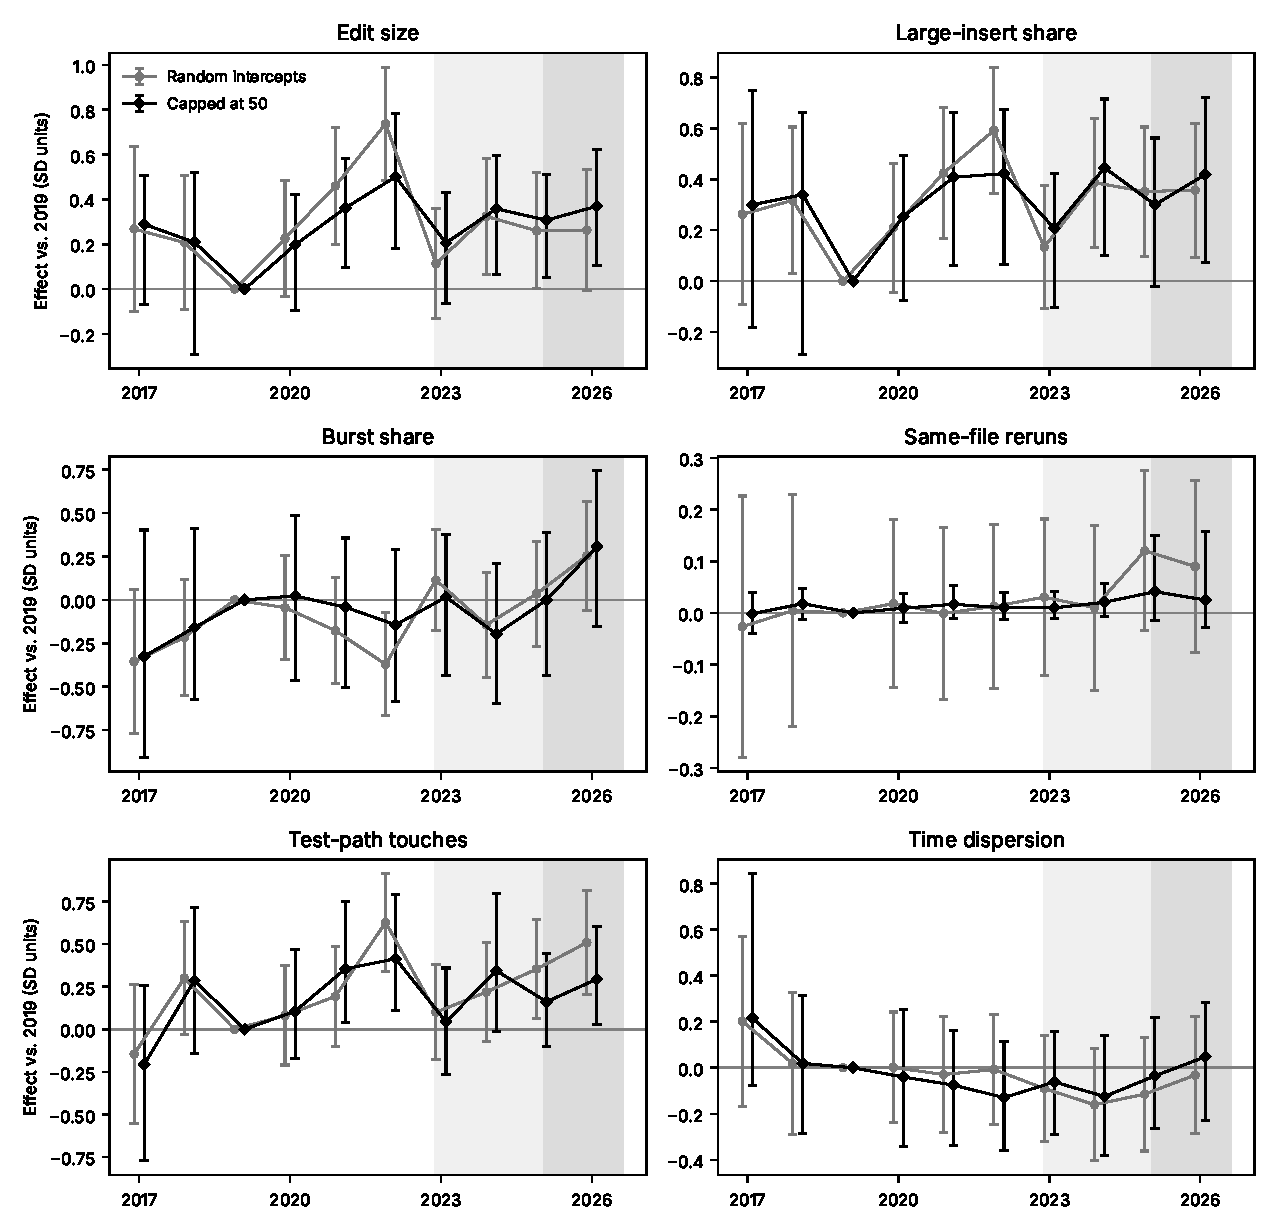
\includegraphics[width=0.85\linewidth,alt={Six line charts of yearly effects from 2017 to 2026 under two estimators, with wide intervals under the capped estimator}]{figs/fig_yearfe_v5}
\caption{Year-of-first-commit effects relative to 2019: gray, organization random intercepts on all repositories (95\% confidence intervals); black, capped at 50 repositories (mean of 200 draws; 95\% intervals from 500 organization-bootstrap replicates). Light band: early post-ChatGPT period; dark band: agentic era.}
\Description{Six line charts with error bars, one per signal. Edit size and large-insert share are high in 2021 and 2022, lower in 2023, and higher again from 2024; test-path touches dip in 2023; the capped intervals are wide.}
\label{fig:yearfe}
\end{figure}

\FloatBarrier
\section{Supplementary Result: Message Distinctiveness}
\label{app:msg}

Message distinctiveness is $1$ minus the mean pairwise cosine similarity of multilingual sentence embeddings (\texttt{multilingual-e5-small}, \citealp{wang2024multilingual}) of a repository's commit messages, after trailer lines are removed; higher means the messages differ more from one another in meaning. It was computed in August 2026 from all non-bot messages of each repository, before the attribution rule existed. The embedding model was not available in the environment of the present analysis, so the signal could not be recomputed on classified commits, and it is reported here rather than in the comparisons. Table~\ref{tab:msg} gives the results. Estimates are expressed in the SD of message distinctiveness in the primary sample of each contrast. In the primary sample, the post-ChatGPT difference is negative in every comparison among all organizations (\R{era.raw.msg} for all repositories, \R{era.capmin.msg} to \R{era.capmax.msg} under the three caps with intervals excluding zero, \R{era.ri.msg} under random intercepts), but the within-organization interval includes zero (\R{era.w.msg}, \R{era.wci.msg}), the difference is smaller in the repositories in which every non-bot commit is classified (\R{msgsub.era.cap50}, \R{msgsub.era.cap50ci}) and in the sample with five or more classified commits (\R{samp-ge5.era.cap50.msg}, \R{samp-ge5.era.cap50ci.msg}), and it is already present for repositories begun in 2021 and 2022 (capped effects relative to 2019 of \R{year.cap.2020.msg} in 2020, \R{year.cap.2021.msg} in 2021, \R{year.cap.2022.msg} in 2022, and \R{year.cap.2023.msg} in 2023; the 2023-versus-2022 contrast is \R{year.cap.c2322.msg}, \R{year.cap.c2322ci.msg}, under the cap and \R{year.ri.c2322.msg}, $p = $ \R{year.ri.c2322p.msg}, under random intercepts). Median message length, standardized by its own SD, shows no post-ChatGPT difference under the cap (\R{extra.era.msg_len_log.cap50}, \R{extra.era.msg_len_log.cap50ci}) but is longer in the agentic era (\R{extra.agent.msg_len_log.cap50}, \R{extra.agent.msg_len_log.cap50ci}), so part of any agentic-era difference in distinctiveness may reflect longer messages. In the agentic era the difference is positive in every comparison among all organizations but its capped intervals include zero (\R{agent.capmin.msg} to \R{agent.capmax.msg}); under random intercepts it is \R{agent.ri.msg}, and \R{agent.loo.msg} without the largest organization; and retaining the assignment copies raises the capped estimate to \R{samp-copies_kept.agent.cap50.msg} (\R{samp-copies_kept.agent.cap50ci.msg}). Because the subset that aligns the messages with classified commits is also a different sample (71\% of pre-era and 89\% of post-era repositories), the weakening in that subset cannot be attributed to the message set alone.

\begin{table}[!htbp]
\caption{Supplementary: message distinctiveness, computed on all non-bot commit messages (not only classified commits), $d$, with 90\% intervals (organization bootstrap for the capped estimates; test inversion for the within-organization estimates, ``none'' where no bound was found). Subset: the repositories in which every non-bot commit is classified, so that the messages coincide with the classified commits' messages; this restriction also changes the sample. All estimates are expressed in the SD of message distinctiveness in the primary sample of the contrast.}
\label{tab:msg}
\scriptsize
\setlength{\tabcolsep}{2.5pt}
\begin{tabular}{@{}p{2.6cm} r c c c r c@{}}
\toprule
Contrast and sample & Raw & Cap 25 & Cap 50 & Cap 100 & RI & Within \\
\midrule
Post $-$ pre, primary & $-0.36$ & $-0.17$ & $-0.17$ & $-0.18$ & $-0.19$ & $-0.10$ \\
 & & $[-0.26, -0.07]$ & $[-0.27, -0.07]$ & $[-0.27, -0.06]$ & & $[-0.38, +0.09]$ \\[2pt]
Agentic $-$ early post, primary & $+0.19$ & $+0.06$ & $+0.08$ & $+0.12$ & $+0.26$ & $+0.45$ \\
 & & $[-0.08, +0.20]$ & $[-0.06, +0.22]$ & $[-0.04, +0.25]$ & & none \\[2pt]
Post $-$ pre, subset (4,021) & $-0.25$ & & $-0.11$ & & $-0.10$ & \\
 & & & $[-0.22, -0.004]$ & & & \\[2pt]
Agentic $-$ early post, subset (2,553) & $+0.25$ & & $+0.12$ & & $+0.24$ & \\
 & & & $[-0.05, +0.24]$ & & & \\[2pt]
\bottomrule
\end{tabular}
\end{table}


\FloatBarrier
\section{Supplementary Analysis: AI Co-authorship Trailers}
\label{app:trailers}

Several AI coding tools append a \textit{Co-authored-by} trailer naming the tool to commits they help produce, and recent mining studies use these trailers, alone or with other Git metadata and repository files, to identify AI-involved commits \citep{khosravani2026census, quispe2026coding, liu2026debt}; related studies identify AI use from explicit self-admissions in commit messages, issues, and pull requests \citep{tufano2026selfadmitted} or from attributions in code comments \citep{mao2026largescale}. For the question of this paper, trailers are another record with its own selection: they come from integrated and agentic tools, not from ChatGPT, and whether a trailer appears depends on which tool is installed and how it is configured. Among repositories with at least three classified commits in the full frame outside test organizations, 0.14\% carried an AI trailer in 2023, 0.18\% in 2024, 1.3\% in 2025, and 8.7\% in the first seven months of 2026. Of the 517 AI-trailer repositories in the model sample below (begun from 2024, five or more classified commits), 81\% name Claude, 11\% Copilot, and 6\% Cursor, and 87\% began in 2026.

A single model with both indicators and year fixed effects is fitted to repositories begun from 2024 in organizations that contain at least one AI-trailer or human-co-author repository (in the full frame, repositories with five or more classified commits; in the primary sample, three or more),
\begin{equation}
y_{ij} = \beta_0 + \beta_{\mathrm{AI}}\,\mathrm{AItrailer}_{ij} + \beta_{\mathrm{H}}\,\mathrm{HumanCoauthor}_{ij} + \text{covariates} + \text{year} + u_j + \varepsilon_{ij},
\label{eq:trailer}
\end{equation}
and the quantity of interest is $\beta_{\mathrm{AI}} - \beta_{\mathrm{H}}$, using human co-author trailers as a placebo convention. The same difference is re-estimated with organization fixed effects and a wild cluster bootstrap. Table~\ref{tab:trailer} and Figure~\ref{fig:trailer} give the results. In the full frame (1,125 repositories in 482 organizations; 517 with AI trailers, 124 with human co-author trailers only), AI-trailer repositories are burstier ($+0.34$), have more distinctive messages ($+0.23$), and are more concentrated in time ($-0.18$, $p = .050$) than other repositories in the model; human-co-author repositories are also burstier ($+0.20$) and more distinctive ($+0.16$), but less concentrated in time ($+0.20$), none of these three distinguishable from zero at the 5\% level ($p = .051$, $.134$, and $.066$). The AI-minus-placebo difference is reliable for time dispersion only ($-0.38 \pm 0.21$; Holm $p = .004$), and larger in the primary sample ($-0.83 \pm 0.40$; 492 repositories, 9 organizations). With organization fixed effects the difference keeps its sign ($-0.57$ and $-0.85$) but rests on 5 and 2 organizations that contain both kinds of repository, and its wild-bootstrap $p$-values are $.10$ and $.21$. The placebo controls for the practice of annotating commits, not for the kind of project in which annotation happens, and the full frame is mostly not coursework. The result is that repositories with AI-tool trailers concentrate their commits in time more than placebo repositories do, and, at the margin of conventional significance, more than other repositories, which is not a demonstration of an AI-specific effect and says nothing about ChatGPT-era students; and the absence of a trailer indicates nothing about AI use.

\begin{table}[!htbp]
\caption{Supplementary: AI-trailer and human-co-author-trailer repositories versus other repositories, first commits 2024 onward, from Equation~\ref{eq:trailer} with organization random intercepts and year fixed effects; full frame: repositories with five or more classified commits; primary sample: three or more. Difference: $\beta_{\mathrm{AI}} - \beta_{\mathrm{H}}$ in SD units with 95\% half-width; $p$ uncorrected and Holm-corrected over the signals. FE: the same difference with organization fixed effects and its wild-cluster-bootstrap $p$ (1,999 replicates).}
\label{tab:trailer}
\scriptsize
\setlength{\tabcolsep}{3pt}
\begin{tabular}{@{}l l l l l l@{}}
\toprule
\multicolumn{6}{@{}l}{Full frame (1,125 repositories, 482 organizations; 517 with AI trailers, 124 with human co-author trailers only)} \\
Signal & AI $d$ ($p$) & Human $d$ ($p$) & Difference & $p$ (Holm) & FE diff.\ ($p_{\text{wild}}$) \\
\midrule
Edit size & $-0.01$ (.911) & $-0.16$ (.090) & $+0.15$ $\pm$ 0.18 & .101 (.607) & $+0.27$ (.327) \\
Large-insert share & $+0.08$ (.293) & $+0.02$ (.828) & $+0.06$ $\pm$ 0.18 & .515 (1) & $+0.26$ (.229) \\
Burst share & $+0.34$ ($<$.001) & $+0.20$ (.051) & $+0.14$ $\pm$ 0.20 & .171 (.855) & $+0.19$ (.790) \\
Same-file reruns & $+0.02$ (.783) & $0.00$ (.967) & $+0.02$ $\pm$ 0.21 & .869 (1) & $+0.01$ (.863) \\
Test-path touches & $-0.04$ (.637) & $+0.04$ (.702) & $-0.08$ $\pm$ 0.20 & .434 (1) & $-0.22$ (.711) \\
Time dispersion & $-0.18$ (.050) & $+0.20$ (.066) & $-0.38$ $\pm$ 0.21 & $<$.001 (.004) & $-0.57$ (.103) \\
Message distinctiveness & $+0.23$ (.009) & $+0.16$ (.134) & $+0.07$ $\pm$ 0.20 & .527 (1) & $+0.16$ (.178) \\
\bottomrule
\end{tabular}

\medskip

\begin{tabular}{@{}l l l l l l@{}}
\toprule
\multicolumn{6}{@{}l}{Primary sample (492 repositories, 9 organizations; 76 with AI trailers, 41 with human co-author trailers only)} \\
Signal & AI $d$ ($p$) & Human $d$ ($p$) & Difference & $p$ (Holm) & FE diff.\ ($p_{\text{wild}}$) \\
\midrule
Edit size & $+0.04$ (.738) & $-0.19$ (.163) & $+0.23$ $\pm$ 0.32 & .156 (.938) & $+0.27$ (.525) \\
Large-insert share & $+0.15$ (.183) & $-0.06$ (.676) & $+0.20$ $\pm$ 0.32 & .207 (.938) & $+0.24$ (.537) \\
Burst share & $+0.40$ (.002) & $+0.14$ (.397) & $+0.26$ $\pm$ 0.37 & .171 (.938) & $+0.26$ (.448) \\
Same-file reruns & $-0.05$ (.728) & $0.00$ (.989) & $-0.05$ $\pm$ 0.42 & .825 (.938) & $-0.04$ (.141) \\
Test-path touches & $-0.10$ (.446) & $+0.12$ (.472) & $-0.23$ $\pm$ 0.39 & .259 (.938) & $-0.28$ (.396) \\
Time dispersion & $-0.42$ (.003) & $+0.41$ (.020) & $-0.83$ $\pm$ 0.40 & $<$.001 ($<$.001) & $-0.85$ (.210) \\
Message distinctiveness & $-0.12$ (.374) & $+0.06$ (.757) & $-0.18$ $\pm$ 0.41 & .389 (.938) & $-0.23$ (.102) \\
\bottomrule
\end{tabular}
\end{table}


\begin{figure}[!htbp]
\centering
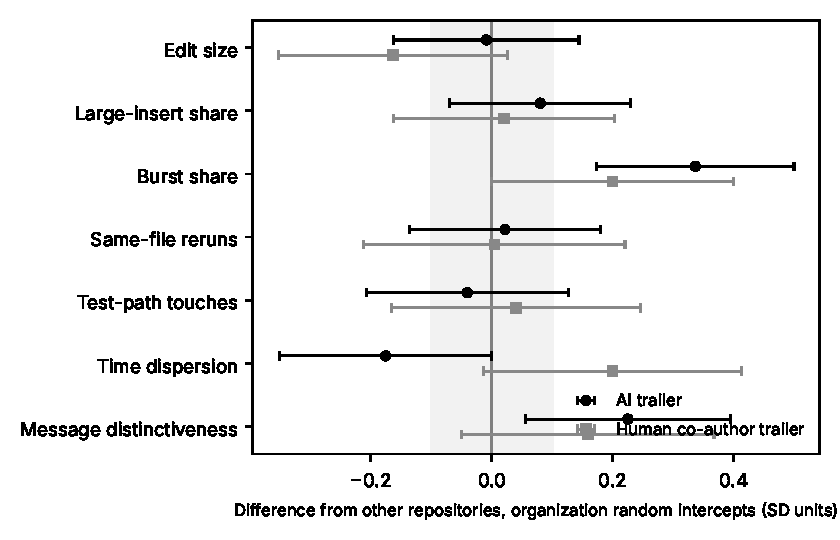
\includegraphics[width=0.6\linewidth,alt={Dot-and-whisker chart of seven signals comparing AI-trailer and human-co-author-trailer repositories with other repositories; AI-trailer estimates are positive for burst share and message distinctiveness and negative for time dispersion; human-co-author estimates are positive for burst share, message distinctiveness, and time dispersion}]{figs/fig_trailer_v4}
\caption{AI-trailer (black) and human-co-author-trailer (gray) repositories versus other repositories, first commits 2024 onward, full frame, from Equation~\ref{eq:trailer} with organization random intercepts and year fixed effects; 95\% confidence intervals, shaded band $\pm 0.10$.}
\Description{Dot-and-whisker chart listing seven signals. AI-trailer estimates are positive for burst share and message distinctiveness and negative for time dispersion. Human-co-author estimates are positive for burst share and message distinctiveness, slightly negative for edit size, and positive for time dispersion.}
\label{fig:trailer}
\end{figure}

\FloatBarrier
\clearpage
\bibliographystyle{ACM-Reference-Format}
\bibliography{refs}

\end{document}
